\makeatletter
\begin{center}
    {\LARGE{\@mytitle}\par}
\end{center}

\begin{center}
    {\@myauthor\par}
\end{center}

\begin{center}
    {\small\@mydate\par}
\end{center}
\makeatother

\begin{abstract}
We study how asymmetric access to consumer data shapes competition and data management strategies in real-time bidding advertising markets. In our model, two demand-side platforms (DSPs) bid for a single ad slot in a first-price auction. Each DSP privately values the impression according to the consumer’s expected interaction with its ad. The DSPs are asymmetrically informed about their values. One DSP is vertically integrated within the ad-tech stack and has privileged access to consumer data: with probability $ \alpha $, it observes its value before bidding; otherwise, it receives the same noisy signal as its non-integrated rival. We characterize the unique Bayesian Nash equilibrium and show that increased access to data softens competition and raises both DSPs' expected payoff. At the same time, consumers benefit from improved targeting. We then allow the integrated platform to license data access to its rival through a take-it-or-leave-it offer. We characterize when the platform optimally preserves a closed ecosystem, offering a formal explanation for the persistence of data silos.
\end{abstract}

\makeatletter
\ifdefempty{\@jelcodes}{}{
\noindent\textbf{JEL Classification:} \@jelcodes
}

\ifdefempty{\@keywords}{}{
\noindent\textbf{Keywords:} \@keywords
}

\noindent \small\@affiliations\par

\ifdefempty{\@acknowledgements}{}{
\noindent \@acknowledgements
}
\makeatother

In many digital markets, platforms have created closed data ecosystems that restrict the flow of information across market participants. The digital display advertising market provides a prominent example. This \$200+ billion industry relies on a complex and highly intermediated infrastructure, called ad-tech stack, in which ad space is bought and sold through automated real-time auctions. When a user visits a webpage, the publisher's ad server identifies an available ad slot and triggers the auction for the corresponding impression. The publisher's supply-side platform (SSP) then makes the impression available to potential buyers through an ad exchange, a digital marketplace where bids are placed in real time. Advertisers rely on DSPs to evaluate the impression and submit bids on their behalf.

Major platforms may operate across several layers of the ad-tech stack, as the example of Google shows. The \textcite{competitionandmarketsauthorityOnlinePlatformsDigital2020} documents that Google controls over 90\% of the ad server market, 50–60\% of the supply-side market, and 50–70\% of the demand side through its various products (see Figure \ref{google-stack}). Beyond its extensive presence in the ad-tech stack, Google operates a broader ecosystem of services that generate rich information about consumers. The combination of consumer-facing services and vertical integration within the ad-tech stack provides Google with a wealth of data that might, in principle, be leveraged to inform the bidding behaviour of its own DSPs.

This is not just a thought experiment: the \textcite{ReGoogleDigital2021} complaint alleges that Google's supply-side ad server shared raw user IDs exclusively with Google-owned DSPs, while providing only hashed identifiers to rival DSPs. These allegations raise a natural question: how does asymmetric access to consumer information shape competition in auction markets? Moreover, why do vertically integrated platforms preserve data silos rather than license data? Given that advertising accounts for the majority of platform revenues, the persistence of closed ecosystems suggests that retaining exclusivity over consumer data at the bidding stage outperforms alternative licensing agreement.

\begin{figure}[h]
    \centering
    \includegraphics[width=1\linewidth]{figures/Fig1-reduced.png}
    \caption{Google's role in advertising intermediation, borrowed from the CMA \citeyear{competitionandmarketsauthorityOnlinePlatformsDigital2020} main report.}
    \label{google-stack}
\end{figure}

To answer these questions, we develop a static model in which two DSPs compete in a first-price auction with a public reserve price to purchase a single ad slot. We assume that each DSP privately values the impression. More precisely, values are i.i.d. discrete random variables representing the uncertain outcome of consumer interaction with the displayed ad. In addition to ensuring tractability, assuming discrete outcomes aligns with how performance campaigns are structured in practice: advertisers define a discrete set of target actions (such as clicks, sign-ups, or purchases) and have a distinct willingness to pay for each\footnote{Modern bidding platforms operationalize this through value-based bidding, which maps predicted consumer outcomes to discrete willingness-to-pay levels. Importantly, the number of discrete valuations in the model corresponds to the granularity of the advertiser's campaign: a campaign targeting a single action features binary outcomes (engagement or no engagement), whereas campaigns targeting richer conversion funnels feature multiple values.}. The assumption of private values that are drawn from the same distribution is best interpreted as considering DSPs bidding on behalf of homogeneous products, with consumers having idiosyncratic tastes. We maintain independence to isolate the effect of information-asymmetry and obtain closed-form solutions, discussing in the appendix how affiliated values would affect our results.

Our baseline model adopts binary valuations: with probability $ p $, the consumer's interaction with the displayed ad generates a high value for the bidder; otherwise, it yields a low value\footnote{The framework extends naturally to $ N $ discrete outcomes, as we show in the appendix.}. We introduce a stark informational asymmetry between the two DSPs. One DSP is vertically integrated with an ad server, while the other is not. With exogenous probability $ \alpha $, the publisher relies on the integrated server to manage its ad inventory. In such case, the server shares consumer-level information with its affiliated DSP, allowing it to observe its private value before bidding. With complementary probability $ 1-\alpha $, both DSPs only know the expected value of the impression. Thus, the parameter $ \alpha $ can be interpreted, to a first approximation, as the share of publishers that rely on the integrated server to manage their ad inventory.

We characterize the unique Bayes-Nash equilibrium of the FPA, in which both bidders randomize over the same interval. More precisely, the integrated DSP's strategy is monotone in its interim valuation: it splits the support into three ordered subintervals -- corresponding to low, expected, and high valuations, in that order. The non-integrated DSP randomizes over the full support with an atom at the reserve price. In equilibrium, both bidders get positive expected revenue, with the integrated DSP earning consistently higher revenue. \par
Equilibrium bidding strategies directly depend on the parameter $ \alpha $, which captures the degree of informational asymmetry. The closed-form expressions we derive allow to easily perform comparative statics. Our main result shows that when $ \alpha $ raises, competition softens and expected revenues of both bidders increase. Such competition softening outcome admits a natural interpretation in terms of mean-preserving spreads: when the integrated DSP is more frequently informed, its behavior becomes more polarized -- aggressive when its value is high, yielding when it is low. This variability benefits the uninformed bidder, who enjoys easy wins when its opponent concedes while facing bounded losses when competition is fierce. On net, both bidders benefit. This monotonicity contrasts with the competition effects of targeting documented in related advertising settings: \textcite{hummelWhenDoesImproved2017} show that in second-price auctions, improved targeting softens competition only beyond a threshold number of bidders, while \textcite{bergemannTargetingAdvertisingMarkets2011} find that equilibrium prices are non-monotone in targeting precision, depending on the degree of market concentration. Note that this competition softening effect would hold even assuming affiliated values. If this were the case, the non-integrated DSP would face a winner's curse, which would make it bid even more conservatively. We maintain independence to isolate the pure information-asymmetry effect and obtain closed-form solutions. In order to measure consumer welfare, we look at the equilibrium probability that consumers engage with the displayed ads. We find that higher values of $ \alpha $ lead to more relevant ads being displayed in equilibrium. \par

\noindent Building on our equilibrium analysis, we ask whether the integrated DSP would ever license data to its rival. To this end, we study arrangements that open the integrated platform's infrastructure: whenever consumer information is available, the competitor is granted access to its own value, while the integrated DSP retains the full informational endowment it derives from owning the infrastructure\footnote{We model the integrated DSP's information set as unchanged under licensing because it owns the data infrastructure through which consumer signals flow: such arrangement can forward those signals to the rival, but it cannot prevent the integrated DSP from reading what passes through its own ad-server.}. We let the integrated platform extract the rival's full willingness to pay for data through a take-it-or-leave-it offer. Even in this extreme benchmark, the integrated platform prefers exclusivity across substantial parameter ranges, and uniformly so once consumers are highly likely to engage with ads ($p \geq \frac{\sqrt{5}-1}{2} \approx 0.62$). The tradeoff is intuitive: licensing brings in a direct payment from the rival but erodes the auction-stage rents that informational asymmetry confers. When consumer engagement is likely, the integrated platform's edge from competing as the sole informed bidder grows faster than the rival's willingness to pay for access. Above $ p \approx 0.62 $, this rent-erosion channel dominates uniformly; below that threshold, exclusivity arises whenever both $ \alpha $ and the reserve price are not too high. The reason is that the expected payoff of the integrated DSP under licensing is linear in $ \alpha $, while under exclusivity it exhibits diminishing returns. Moreover, licensing is associated with high reserve prices because then the rival DSP is willing to pay more to avoid overspending on low-value impressions.

To the best of our knowledge, our investigation provides the first formal explanation for why vertically integrated ad-tech platforms such as Google maintain closed data ecosystems. We characterise the precise boundary conditions under which this logic applies. We conclude our analysis with a calibration exercise providing evidence, in the context of click campaigns, that the parameter range where exclusivity dominates licensing reflects current market conditions.

\noindent The remainder of the paper is organised as follows. Section \ref{sect:lit} reviews the related literature. Section \ref{baseline-model} introduces the model, characterises the unique Bayes-Nash equilibrium, and derives the comparative statics with respect to the information-asymmetry parameter $\alpha$. Section \ref{licensing} studies the mandated data-sharing remedy and characterises the parameter region in which the integrated platform prefers to keep a closed ecosystem. Subsection \ref{sect:calibration} calibrates the model to click-campaign data and shows that this region is empirically relevant. Section \ref{sect:conclusion} concludes. Proofs and robustness extensions are collected in the appendix.
\section{Literature}\label{sect:lit}
\noindent Our focus on FPA reflects the current state of open display advertising markets. Through the 2010's, ad exchanges progressively moved from second-price to first-price auction formats. \textcite{despotakisFirstPriceAuctionsOnline2021} trace this shift to the widespread adoption of header bidding, whereby publishers broadcast bid requests to multiple exchanges simultaneously rather than sequentially. They show that, once publishers adopt header bidding, all exchanges switching to FPA is the unique equilibrium of the game. Consistent with this prediction, Google completed its transition to first-price rules in 2019, making FPA the standard across all major open exchanges.\footnote{See Google's \href{https://blog.google/products/admanager/update-first-price-auctions-google-ad-manager/}{blog announcement}. See also \href{https://developers.google.com/authorized-buyers/rtb/start}{Google's Real-Time Bidding guide}, which states: ``The bid response is received and its bid enters the open auction, where it wins the impression because it is the highest bid". Walled-garden platforms where the exchange and publisher are vertically integrated (e.g., Amazon, Facebook) may retain second-price formats for their own inventory \parencite{choiOptimizingReservePrices2023}. Our model studies DSPs competing through an independent exchange, which is the setting where FPA is now universal.} \textcite{alcobendasSlimShadingAd2021} provide auction-level empirical evidence from the Yahoo Ad Exchange's contemporaneous switch to first-price rules, documenting how DSPs adjusted their bid-shading strategies in response. From a theoretical perspective, \textcite{lemeWhyCompetitiveMarkets2020} establish that FPA is the unique Nash equilibrium in a static game between competing exchanges, offering a complementary rationale for the industry-wide convergence. FPA is also considered more transparent, as there is no uncertainty in the final price upon winning. \textcite{dengNonuniformBidscalingEquilibria2024} further show, through simulations of optimal bidding in an environment populated by autobidders, that FPA dominates both second-price and Vickrey-Clarke-Groves auctions in terms of bidders' welfare as well as auctioneer's profits. In the sponsored-search context, \textcite{kimNonparametricEstimationSponsored2025} nonparametrically estimate advertiser valuations in weighted GSP auctions using Yahoo! data and show through counterfactuals that product-specific quality scoring can substantially raise search-engine revenue at the expense of advertiser profits and ad quality.\par

\noindent The theoretical literature on asymmetric first-price auctions (FPAs) distinguishes between two main sources of asymmetry. The first strand examines ex-ante distributional asymmetries, where bidders draw valuations from distributions that differ in their stochastic properties. \textcite{maskinAsymmetricAuctions2000} provide seminal results characterizing equilibria when value distributions are stochastically ordered. The second strand considers informational asymmetries with a common prior, where bidders share the same ex-ante value distributions but differ in their information about realized values. Within this informational asymmetry literature, most work has focused on common value settings, starting with \textcite{wilsonCompetitiveBiddingAsymmetric1967} and \textcite{engelbrecht-wiggansCompetitiveBiddingProprietary1983}, with more recent contributions such as \textcite{abrahamPeachesLemonsCookies2020} studying second-price auctions. The literature on FPAs with independent private values (IPV) and informational asymmetries is comparatively smaller: either all players know their own values \parencite{martinez-pardinaFirstpriceAuctionsWhere2006}, or the focus is on alternative auction formats \parencite{compteWaitandSeeOptionAscending2004, miettinenInformationAcquisitionDutch2013}. A growing body of work examines information acquisition in FPAs, though with IPV this literature has primarily focused on symmetric strategies \parencite{hauschPrivateValuesAuctions1991, shiOptimalAuctionsInformation2012}. \textcite{bergemannFirstPriceAuctionsGeneral2017} characterize equilibrium behavior across general information structures, providing bounds on winning bid distributions and revenues.\par

\noindent We contribute to the second strand by characterizing a closed-form mixed-strategy equilibrium for FPAs with IPV under structural informational asymmetries. This specific setting, in which one bidder may privately observe realized values while the other remains uninformed, is motivated by applications to digital advertising markets and analytical tractability. In programmatic advertising, vertically integrated platforms can observe consumer preferences through their broader digital ecosystem, creating precisely the type of interim informational advantage we model. From an ex-ante perspective, the resulting preference structure fits the framework of \textcite{maskinAsymmetricAuctions2000}, with the informed bidder's value distribution first-order stochastically dominating that of the uninformed bidder. This tractability allows us to derive explicit comparative statics and welfare implications, providing a foundation for analyzing competitive effects of data advantages in auction settings.\par

\noindent Closest in spirit to our work is \textcite{abrahamPeachesLemonsCookies2020}, who study auction markets with dispersed information in the context of online advertising. Their framework features bidders with affiliated values and focuses primarily on second-price auctions, characterizing conditions under which the informed platform prefers to share information with competitors. Relatedly, \textcite{arnostiAdverseSelectionAuction2016} show that when bidder values are positively correlated, second-price auctions for display advertising expose uninformed advertisers to adverse selection, and introduce modified second-bid auctions as a mechanism design response. Our setting differs in two key respects. First, we analyze first-price auctions, which have become the dominant format in display advertising. Second, we work with independent private values: vertically integrated platforms can access fine-grained behavioral data, such as detailed browsing history, that reveals idiosyncratic consumer preferences for specific products. This granular information generates value that is plausibly independent across competing DSPs, in contrast to the common value component arising from aggregate ad effectiveness. The IPV structure, combined with our focus on first-price auctions, yields qualitatively different equilibrium dynamics, notably the necessity of mixed strategies and the non-monotonic relationship between information asymmetry and competitive intensity. While Abraham et al. find that information sharing can arise as an equilibrium outcome under second-price rules, our analysis identifies conditions under which closed data ecosystems are strictly optimal under first-price competition, providing a complementary explanation for observed platform behavior.\par

\noindent On the vertical integration dimension, \textcite{dannunzioDigitalEcosystemsAdtech2024} study how vertical integration between a publisher and a supply-side intermediary affects competing publishers' revenue and content quality provision. Under diminishing returns to advertising to the same consumer, the integrated intermediary can observe whether consumers visiting the independent publisher are multi-homers who also visit the integrated one, and efficiently manages the frequency of ad exposure. We look at vertical integration spanning the full stack from demand to supply side, and provide a micro-founded analysis of the auction mechanism in light of information asymmetries on the supply side. \textcite{dannunzioIntermediariesOnlineAdvertising2024} examine how ad intermediaries strategically choose whether to disclose consumer information to advertisers when selling ad impressions. Here too, consumers multi-home and returns to advertising are diminishing. They find that when advertising markets are ``thin" (few advertisers targeting a specific consumer type), intermediaries prefer to make targeting less granular to maintain higher ad prices, rather than withholding information about cross-publisher ad exposure. More broadly, our analysis of closed data ecosystems relates to general theories of digital ecosystems, such as \textcite{rhodesDigitalEcosystemsData2024} and \textcite{heidhuesTheoryDigitalEcosystems2024}. \par

\section{Model}\label{baseline-model}
\subsection{Setup}

\noindent \textit{Bidders} -- Two DSPs, denoted $ d_1 $ and $ d_2 $, compete in a first-price auction for a single indivisible ad-slot. The auction has an exogenous reserve price $ r > 0 $, which is common knowledge. The private value of the ad-slot for $ d_i $ is $ v_i \in \{ v_L, v_H \} $, where $ 0 \leq v_L < v_H $. Valuations $ v_1, v_2 $ are independently and identically distributed, with
\begin{equation*}
 \mathbb{P}(v_i = v_H) = p \in (0,1).
\end{equation*}

\noindent We denote $ \mu := \mathbb{E}(v_i) $ and we assume $ \mu > r$. The parameter $ p $ represents the probability that a consumer engages with the displayed ad in the manner targeted by the campaign. In our baseline specification, we interpret engagement as a click, corresponding to a binary performance campaign; the extension to richer outcome spaces is immediate (see Appendix \ref{sect:N-values}). \\

\noindent \textit{Information} -- DSPs have asymmetric information about valuations. We assume that $ d_1 $ is vertically integrated within the ad-tech stack, and thus observes the realization of both valuations $ (v_1, v_2) $ with exogenous probability $ \alpha \in [0,1] $; with complementary probability $ 1 - \alpha $, it only knows the distribution of values\footnote{Assuming that $ d_1 $ observes both valuations is without loss of generality in our setting: $ d_1 $'s payoff depends only on $ v_1 $, and $ d_2 $'s strategy does not condition on $ v_2 $ since $ d_2 $ is uninformed. However, introducing $ d_1 $'s observation of $ v_2 $ from the outset provides a natural foundation for the data licensing analysis in Section~\ref{licensing}, where $ d_1 $ may choose to share information about $ v_2 $ with $ d_2 $.}. Accordingly, the type of $ d_1 $ is
\begin{equation*}
 t_1 \in T_1 := \{ v_L, v_H, \mu \},
\end{equation*}

\noindent where $ t_1 = v_i $ indicates that $ d_1 $ is informed that its valuation is $ v_i $, and $ t_1 = \mu $ represents the case where it did not observe the realization of values. The induced distribution over $ d_1 $'s types is
\begin{equation*}
\mathbb{P}(t_1 = v_L) = \alpha(1 - p), 
\mathbb{P}(t_1 = v_H) = \alpha p, 
\mathbb{P}(t_1 = \mu) = 1 - \alpha.
\end{equation*}

\noindent We assume $ d_2 $ only knows the distribution of valuations. Consequently, it always values the ad-slot at $ \mu $. \\

\noindent \textit{Timing} -- Nature draws $ (v_1, v_2) $ and determines whether $ d_1 $ observes realizations or not. DSPs simultaneously place their bids. The highest bid above the reserve price $ r $ wins the auction. If no bid exceeds the reserve price, the object remains unassigned. Draws are solved with a fair coin toss. \\

\noindent \textit{Strategies and Payoffs} -- We assume that a bidder never bids above his valuation. The strategy of $ d_1 $ is a type-contingent collection
\begin{equation*}
 \overline{\sigma}_1 := \left(\sigma_1^{t_1}\right)_{t_1 \in T_1},
\end{equation*}

\noindent where $ \sigma_1^{t_1} \in \Delta\left([0, t_1]\right) $ denotes the strategy played by $ d_1 $ when its type is $ t_1 \in T_1 $. We denote $ F_1^{t_1} $ the c.d.f. associated to $ \sigma_1^{t_1} $. The strategy of $ d_2 $ is denoted $ \sigma_2 $, with $ F_2 $ the associated c.d.f. The expected utility of $ d_1 $ if its type is $ t_1 $ and $ \left( \overline{\sigma}_1, \sigma_2 \right) $ is played is\footnote{DSPs' payoff function reflects their incentive to act in advertisers' best interest: a DSP trades off the fee gained from consumer engagement ($t_i$) against the cost of acquiring an impression ($b$).}
\begin{equation*}
 \mathbb{E}\tilde{u}_1 \left( \overline{\sigma}_1, \ \sigma_2 \ \big| \ t_1  \right) := \int_{r}^{\infty} (t_1 - b) F_2(b) d F_1^{t_1}(b).
\end{equation*}

\noindent  The expected utility of $ d_2 $ when $ \left( \overline{\sigma}_1,\ \sigma_2 \right) $ is played is
\begin{equation*}
\mathbb{E}\tilde{u}_2 \left( \sigma_2,\ \overline{\sigma}_1 \right) := \int_{r}^{\infty} (\mu - b) \left[ \alpha (1 - p) F_1^{v_L}(b) + \alpha p F_1^{v_H}(b) + (1 - \alpha) F_1^{\mu}(b) \right] d F_2(b)
\end{equation*}

\noindent We solve for a Bayesian Nash equilibrium of this first-price auction.

\subsection{Equilibrium Analysis}
\noindent We characterize the unique equilibrium of the asymmetric information game in three steps. First, we establish that no pure strategy equilibrium exists. Second, we derive necessary conditions on the support structure of equilibrium distributions. Third, we construct the equilibrium distributions explicitly and verify uniqueness.

\noindent In the following, we restrict attention to the case in which $v_L < r$. Given that bidders never bid above their valuations, it is without loss to assume that $d_1$ drops out of the auction whenever $t_1 = v_L$. We will show that the reserve price anchors the lower bound of equilibrium bidding supports.\footnote{See \textcite{lizzeriUniquenessExistenceEquilibrium2000} for a general treatment of reserve prices in asymmetric auctions with affiliated signals. Note also that a public reserve price prevents mechanism credibility issues \parencite{banchioDynamicThreatsCredible}.} The case where all valuations exceed the floor price yields an isomorphic structure with the anchor shifted from $r$ to $v_L$ (Appendix \ref{sect:nonbinding-floor}).

\noindent The FPA does not admit an equilibrium in pure strategies. The key driver is that $ d_2 $ is always uninformed: her effective valuation is degenerate at $ \mu $. In a first-price auction, any pure bid by a single-type player becomes a fixed target for opponent types with valuations exceeding the bid, who can profitably $ \epsilon $-overbid. This forces $ d_2 $ to randomize. The result does not depend on $ d_1 $'s valuations being discrete; see Appendix \ref{sect:continuous-values} for the continuous-valuations case.

\begin{prop}\label{prop:no-pure}
There exists no equilibrium in pure strategies.
\end{prop}

\begin{proof}
\noindent Let $ \overline{b}_1 = \left(b_1^{v_H},\ b_1^{\mu}\right) \in [0, v_H] \times [0, \mu] $ be a pure strategy of $ d_1 $ . Given a type $ t_1 \in \{ v_H, \mu \} $, the payoff of $ d_1 $ if he plays $ \overline{b}_1 $ and $ d_2 $ plays $ b_2 \in [0, \mu] $ is:

\begin{equation*}
\tilde{u}_1(\overline{b}_1,\ b_2 \ | \ \ t_1) = \left( t_1 - b_1^{t_1} \right) \mathbb{1}\left( b_1^{t_1} > \max\{b_2, r\} \right)
\end{equation*}

\noindent The expected payoff for $ d_2 $ is

\begin{equation*}
 \mathbb{E}\tilde{u}_2 \left(b_2,\ \overline{b}_1 \right) = (\mu - b_2) \left[ \alpha (1 - p) + \alpha p \mathbb{1}\left(b_2 > \max\{b_1^{v_H}, r\}\right) + (1 - \alpha) \mathbb{1}\left(b_2 > \max\{b_1^{\mu}, r\}\right) \right].
\end{equation*}

\noindent Assume that in equilibrium $ d_2 $ plays the pure strategy $ b_2 \in [0, \mu] $. If $ t_1 = v_H $ we claim that there exists no best response of $ d_1 $ to $ b_2 $. Indeed, for any $ \varepsilon > 0 $ arbitrarily small, playing $ b_2 + \varepsilon $ is a profitable deviation for $ d_1 $. Therefore, in any equilibrium $ d_2 $ must play a mixed strategy. Now assume that $ d_1 $ plays the pure strategy $ \overline{b}_1 $ and let $ F_2 $ be the c.d.f. associated to the mixed strategy $ \sigma_2 $ of $ d_2 $. In equilibrium, $ d_2 $ must be indifferent across all bids $ b_2 \in Supp(F_2) $. Formally, there exists a constant $ k > 0 $ such that $ \forall b_2 \in Supp(F_2) $

\begin{equation*}
 (\mu - b_2) \left[ \alpha (1 - p) + \alpha p \mathbb{1}\left( b_2 > \max\{b_1^{v_H}, r\}\right) + (1 - \alpha) \mathbb{1}\left(b_2 > \max\{b_1^{\mu}, r\} \right) \right] = k.
\end{equation*}

\noindent For any $ k > 0 $, there exists at most a finite number of $ b_2 \in [0, \mu] $ satisfying the indifference condition above. Therefore, $ Supp(F_2) $ must be a finite set. But then $ d_1 $ could profitably deviate by $ \epsilon $ overbidding $ d_2 $.

\end{proof}

\noindent We now focus on mixed strategies equilibria. In the following, we provide necessary conditions that pin down the structure of candidate equilibria, gradually building intuition. Let us define:

\[
\underline{b_2} = inf\left(Supp\left(F_2\right)\right),  \overline b_2 = sup\left(Supp\left(F_2\right)\right),
\]

\noindent and for $ t_1 \in \{ v_H, \mu \} $

\[
\underline{b}_1^{t_1} = inf\left(Supp\left(F_1^{t_1}\right)\right),  \overline{b}_1^{t_1} = sup\left(Supp\left(F_1^{t_1}\right)\right).
\]

\noindent We can resort to two classical results in first-price auctions literature, established by \textcite{maskinEquilibriumSealedHigh2000}.\footnote{\noindent All relevant conditions are satisfied:
\begin{itemize}
    \item[-] \textit{Monotonicity}: Payoffs are strictly increasing in own type. For $ d_1 $, since $ c > \mu $, type $ v_H $ has strictly higher value than type $ v_L $. For $ d_2 $, the condition is vacuously satisfied.
    \item[-] \textit{Weak supermodularity}: Follows from risk neutrality.
    \item[-] \textit{Private values}: Each bidder's payoff depends only on their own type.
    \item[-] \textit{Affiliation}: Since $ d_2 $ has a degenerate type, the joint distribution over types is determined entirely by the marginal over $ t_1 $. The affiliation condition is thus trivially satisfied.
\end{itemize}
} First, in equilibrium there must be a form of monotonicity in the bidding behavior of $ d_1 $. More precisely, $ d_1 $ always bids higher when $ t_1 = v_H $ compared to when $ t_1 = \mu $. Secondly, the support of the equilibrium distribution of winning bids must be an interval, with no mass points in its interior.

\begin{lem}\label{lem:monotonicity}
Let $ \left(F_1^{v_H}, F_1^{\mu}, F_2 \right) $ be an equilibrium of the FPA. Then we have:

\begin{equation*}
\overline{b}_1^{\mu} \leq \underline{b}_1^{v_H}
\end{equation*}
\end{lem}
\begin{proof}
    Follows from \textcite{maskinEquilibriumSealedHigh2000}, Proposition 1.
\end{proof}

\begin{lem}\label{lem:interval}
Let $ W \subseteq [r, \mu] $ be the support of the distribution of winning bids in a given equilibrium $ \left(F_1^{v_H}, F_1^{\mu}, F_2\right) $. Then, $ W = [\underline b, \overline{b}] $ with $ r \leq \underline{b} < \overline {b} \leq \mu $. Moreover, there are no mass points in $ (\underline b, \overline b) $.
\end{lem}
\begin{proof}
    Follows from \textcite{maskinEquilibriumSealedHigh2000}, Proposition 3.
\end{proof}

\noindent Given these general results, we can further pin down the structure of an equilibrium in our framework. More precisely, we can characterize the shape of equilibrium distributions' supports.

\begin{prop}\label{prop:eqm-supports}
Let $ \left(F_1^{v_H}, F_1^{\mu}, F_2 \right) $ be an equilibrium of the FPA. Then:

\begin{itemize}
    \item[-] $ Supp(F_2) = [r, \overline b] $ for some $ \overline{b} \in (r, \mu) $.

    

    \item[-] $ Supp\left(F_1^{\mu}\right) = [r, \hat{b}] $ for some $ \hat{b} \in (r, \overline b) $.

    

    \item[-] $ Supp\left(F_1^{v_H}\right) = [\hat{b}, \overline{b}] $.
\end{itemize}
\end{prop}

\noindent In equilibrium, the two bidders mix over a common support $ [r, \overline b] $. $ d_2 $ mixes across the whole interval, whereas $ d_1 $ splits such interval into two, ordered subintervals: he plays in the lower subinterval $ [r, \hat{b}] $ when $ t_1 = \mu $, whereas he mixes in the upper subinterval $ [\hat{b}, \overline{b}] $ when $ t_1 = v_H $. The figure below illustrates the shape of supports in a candidate equilibrium.

\begin{center}

\tikzset{every picture/.style={line width=0.75pt}}

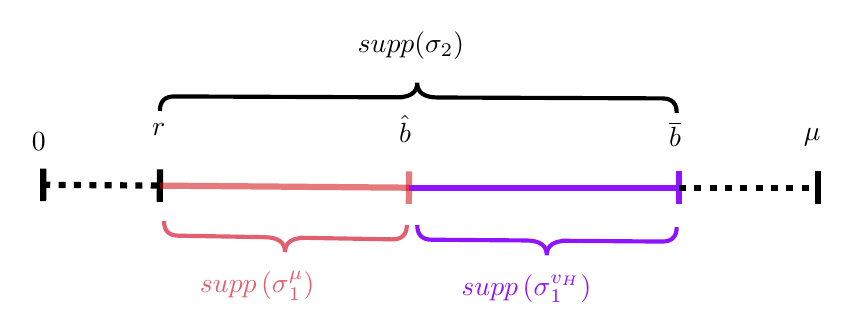
\begin{tikzpicture}[x=0.75pt,y=0.75pt,yscale=-1,xscale=1]

\draw [line width=2.25]  [dash pattern={on 2.53pt off 3.02pt}]  (144,93.2) -- (200.2,93.6) ;
\draw [shift={(200.2,93.6)}, rotate = 180.41] [color={rgb, 255:red, 0; green, 0; blue, 0 }  ][line width=2.25]    (0,7.83) -- (0,-7.83)   ;
\draw [shift={(144,93.2)}, rotate = 180.41] [color={rgb, 255:red, 0; green, 0; blue, 0 }  ][line width=2.25]    (0,7.83) -- (0,-7.83)   ;
\draw [color={rgb, 255:red, 208; green, 2; blue, 5 }  ,draw opacity=0.53 ][line width=2.25]    (200.2,93.6) -- (320.2,94.6) ;
\draw [shift={(320.2,94.6)}, rotate = 180.48] [color={rgb, 255:red, 208; green, 2; blue, 5 }  ,draw opacity=0.53 ][line width=2.25]    (0,7.83) -- (0,-7.83)   ;
\draw [color={rgb, 255:red, 144; green, 19; blue, 254 }  ,draw opacity=1 ][line width=2.25]    (320.2,94.6) -- (450.2,94.6) ;
\draw [shift={(450.2,94.6)}, rotate = 180] [color={rgb, 255:red, 144; green, 19; blue, 254 }  ,draw opacity=1 ][line width=2.25]    (0,7.83) -- (0,-7.83)   ;
\draw [line width=2.25]  [dash pattern={on 2.53pt off 3.02pt}]  (450.2,94.6) -- (517.2,94.6) ;
\draw [shift={(517.2,94.6)}, rotate = 180] [color={rgb, 255:red, 0; green, 0; blue, 0 }  ][line width=2.25]    (0,7.83) -- (0,-7.83)   ;
\draw  [color={rgb, 255:red, 208; green, 2; blue, 27 }  ,draw opacity=0.63 ][line width=1.5]  (202.2,110.6) .. controls (202.12,115.27) and (204.41,117.64) .. (209.08,117.72) -- (250.58,118.43) .. controls (257.25,118.54) and (260.54,120.93) .. (260.46,125.6) .. controls (260.54,120.93) and (263.91,118.66) .. (270.58,118.77)(267.58,118.72) -- (312.08,119.48) .. controls (316.75,119.56) and (319.12,117.27) .. (319.2,112.6) ;
\draw  [color={rgb, 255:red, 144; green, 19; blue, 254 }  ,draw opacity=1 ][line width=1.5]  (324.2,112.6) .. controls (324.16,117.27) and (326.47,119.62) .. (331.14,119.66) -- (376.64,120.02) .. controls (383.31,120.07) and (386.62,122.43) .. (386.59,127.1) .. controls (386.62,122.43) and (389.97,120.13) .. (396.64,120.18)(393.64,120.16) -- (442.14,120.55) .. controls (446.81,120.58) and (449.16,118.27) .. (449.2,113.6) ;
\draw  [line width=1.5]  (449.2,58.6) .. controls (449.22,53.93) and (446.9,51.59) .. (442.23,51.57) -- (334.17,51.14) .. controls (327.5,51.11) and (324.18,48.77) .. (324.2,44.1) .. controls (324.18,48.77) and (320.84,51.09) .. (314.17,51.06)(317.17,51.07) -- (207.23,50.63) .. controls (202.56,50.61) and (200.22,52.93) .. (200.2,57.6) ;

\draw (137,66.4) node [anchor=north west][inner sep=0.75pt]    {$0$};
\draw (195,62.4) node [anchor=north west][inner sep=0.75pt]    {$r$};
\draw (314,58.4) node [anchor=north west][inner sep=0.75pt]    {$\hat{b}$};
\draw (444,61.4) node [anchor=north west][inner sep=0.75pt]    {$\overline{b}$};
\draw (509,64.4) node [anchor=north west][inner sep=0.75pt]    {$\mu$};
\draw (218,133.4) node [anchor=north west][inner sep=0.75pt]  [color={rgb, 255:red, 208; green, 2; blue, 27 }  ,opacity=0.63 ]  {$supp\left( \sigma {_{1}^{\mu}}\right)$};
\draw (344,135) node [anchor=north west][inner sep=0.75pt]  [color={rgb, 255:red, 144; green, 19; blue, 254 }  ,opacity=1 ]  {$supp\left( \sigma {_{1}^{v_H}}\right)$};
\draw (294,18) node [anchor=north west][inner sep=0.75pt]  [color={rgb, 255:red, 0; green, 0; blue, 0 }  ,opacity=1 ]  {$supp( \sigma _{2})$};
\end{tikzpicture}
\end{center}

\subsubsection{Proof of the Proposition}

In order to prove Proposition \ref{prop:eqm-supports}, we resort to the following intermediate results.

\begin{lem}\label{lem:bounds}
In any equilibrium we have:

\begin{enumerate}

    \item $ \overline{b}_2 = max \left\{ \overline{b}_1^{v_H}, \overline{b}_1^{\mu} \right\}$.

    

    \item $ r = \underline{b}_2 \leq \underline{b}_1^{\mu} $.
\end{enumerate}
\end{lem}

\begin{proof}
The first claim is trivial. In equilibrium, no player ever bids strictly more than the highest bid of his opponent.

\noindent To prove the second claim, first notice that it is easy to show that in equilibrium $ \underline{b}_2 \leq \underline{b}_1^{\mu} $. If not, then $ d_1 $ would get an expected payoff of zero from bids in $ (\underline{b}_1^{\mu}, \underline{b}_2) $ when his type is $ \mu $. We next show that $ \underline{b}_2 = r $. By contradiction let $ \underline{b}_2 > r $. Then we would have:
\begin{equation*}
r < \underline{b}_2 \leq \underline{b}_1^{\mu}
\end{equation*}

\noindent If we had $ \underline{b}_2 < \underline{b}_1^{\mu} $, then clearly $ d_2 $ could profitably deviate to $ r $: the probability of winning would always be $ \alpha (1 - p) $ but the markup would increase. If instead we had $ \underline{b}_2 = \underline{b}_1^{\mu} = \underline{b} $, we argue that $ \underline b $ could not be a mass point for $ d_1 $. Indeed, if $ \underline b $ was a mass point for $ d_1 $, then clearly it could not be a mass point also for $ d_2 $: any of the two bidders would profitably shift such a mass to $ \underline{b} + \varepsilon $. But then $ d_1 $ would be putting a mass on a bid at which he earns zero expected profits, which can not happen in equilibrium. Given that $ \underline b $ can not be a mass point for $ d_1 $, again $ d_2 $ could profitably deviate to $ r $. This shows that $ \underline{b}_2 = r $ in equilibrium.
\end{proof}

\begin{lem}\label{lem:inclusion}
In equilibrium, $ supp \left( F_1^{t_1} \right) \subseteq supp \left(F_2\right) $ for all $ t_1 \in \{ v_H, \mu \} $.
\end{lem}

\begin{proof}
 By contradiction, suppose there exists $ \tilde{b} \in Supp\left(F_1^{t_1}\right) \setminus Supp(F_2) $. Then it must be $ \tilde b > r $. Let $ \varepsilon > 0 $ be such that no bid in $ (\tilde b - \varepsilon,\ \tilde b) $ is contained in $ Supp(F_2) $. We claim that $ d_1 $ could profitably deviate to $ \tilde b - \varepsilon $ when $ t_1 \in \{ v_H, \mu \} $. Indeed, the probability of winning for $ d_1 $ would be unaffected, and the markup for $ d_1 $ is higher at $ \tilde b - \varepsilon $ than at $ \tilde b $.
\end{proof}

\begin{lem}\label{lem:lowest}
In equilibrium, we have $ \underline{b}_1^{\mu} = r $.
\end{lem}

\begin{proof}
By contradiction, assume that $ \underline{b}_1^{\mu} > r $. Then, no bid in $ \left[r,\ \underline{b}_1^{\mu}\right] $ is contained in $ Supp\left(F_1^{\mu}\right) $. From the previous lemma, we know that $ \underline{b}_1^{\mu} \in Supp(F_2) $. Therefore, in equilibrium $ d_2 $ must be indifferent between $ r $ and $ \underline{b}_1^{\mu} $

\begin{align*}
&\underbrace{(\mu - r)\alpha(1-p)}_\text{$ \mathbb{E}\tilde{u}_2(r,\ F_1^{\mu}, F_1^{v_H})$} = \underbrace{(\mu - \underline{b}_1^{\mu})\left(\alpha(1 - p) + (1 - \alpha) F_1^{\mu}(\underline{b}_1^{\mu}) \right)}_\text{$ \mathbb{E}\tilde{u}_2(\underline{b}_1^{\mu},\ F_1^{\mu}, F_1^{v_H})$}\\[5pt]
\iff \ &F_1^{\mu}(\underline{b}_1^{\mu}) > 0
\end{align*}

\noindent Thus, $ \underline{b}_1^{\mu} $ should be a mass point for $ d_1 $, which contradicts the fact that there are no interior mass points in the support of the equilibrium winning bid distributions. As a consequence, we must have $ \underline{b}_1^{\mu} = r $.
\end{proof}

\begin{lem}\label{lem:union}
In equilibrium we have $ Supp(F_2) = Supp\left(F_1^{v_H}\right) \cup Supp\left(F_1^{\mu}\right) $
\end{lem}

\begin{proof}
It suffices to show that $ supp(F_2) \subseteq Supp\left(F_1^{v_H}\right) \cup Supp\left(F_1^{\mu}\right) $. By contradiction, suppose there exists $ \tilde{b} \in supp(F_2) $ such that $ \tilde{b} \notin Supp\left(F_1^{t_1}\right) $ for $ t_1 \in \{ \mu,\ v_H \} $. Then, there exists $ \varepsilon > 0 $ such that $ (\tilde{b} - \varepsilon,\ \tilde{b}) $ is not contained in $ Supp\left(F_1^{v_H}\right) \cup Supp\left(F_1^{\mu}\right) $. We claim that $ d_2 $ could profitably deviate to $ \tilde{b} - \varepsilon $. Indeed, the winning probability would be unaffected, and the markup for $ d_2 $ is higher at $ \tilde{b} - \varepsilon $ than at $ \tilde{b} $.
\end{proof}

\noindent We can now put together all the intermediate results, and prove the proposition.

\begin{proof}
We showed that

\begin{equation*}
 Supp(F_2) = Supp\left(F_1^{v_H}\right) \cup Supp\left(F_1^{\mu}\right) = [\underline b, \overline b] \subseteq [r, \mu].
\end{equation*}

\noindent Moreover, we showed that $ \underline b = r $. Since we know that $ \overline{b}_1^{\mu} \leq \underline{b}_1^{v_H} $, it must be that

\begin{align}\label{eq:supp-d1}
Supp\left(F_1^{\mu}\right) = \left[r,\ \overline{b}_1^{\mu}\right],  Supp\left(F_1^{v_H}\right) = \left[\overline{b}_1^{\mu}, \overline b\right]
\end{align}

\noindent and consequently:

\begin{equation}\label{eq:supp-d2}
 Supp(F_2) = [r, \overline{b}].
\end{equation}

\end{proof}

\noindent We can now characterize the unique BNE that satisfies the necessary conditions provided so far.

\begin{prop}\label{mixed-BNE-main}

There exists a unique BNE in completely mixed strategies $ \left( \left( \sigma_1^{v_H^*},\ \sigma_1^{\mu^{*}} \right), \ \sigma_2^* \right) $ where the associated C.D.F.s are given by:

{\footnotesize
\begin{equation*}
 F_1^{v_H^*}(b) = \begin{cases}
     0, & b < \hat{b} \\[5pt]
     \frac{1}{\alpha p} \left( \frac{\alpha (1 - p)(\mu - r)}{\mu - b} - (1 - \alpha p) \right), & b \in \left[ \hat{b},\ \overline{b} \right] \\[5pt]
     1, & b > \overline{b}
 \end{cases},  F_1^{\mu^*}(b) = \begin{cases}
     0, & b < r \\[5pt]
     \frac{1}{1 - \alpha} \left( \frac{\alpha (1 - p)(\mu - r)}{\mu - b} - \alpha (1 - p) \right), & b \in \left[ r,\ \hat{b} \right] \\[5pt]
     1, & b > \hat{b}
 \end{cases}
\end{equation*}
}

\begin{small}
\begin{equation*}
 F_2^*(b) = \begin{cases}
        0, & b < r \\[5pt]
        \frac{\alpha (1 - p) (\mu - r) \left[ c +\alpha (\mu - r) \right]}{(v_H - \alpha r)(\mu - b)}, &  b \in \left[ r, \ \hat{b} \right] \\[5pt]
        \frac{(1 - p)[v_H + \alpha (\mu - r)]}{v_H - b},  & b \in \left[ \hat{b}, \ \overline{b} \right] \\[5pt]
        1, & b > \overline{b}
    \end{cases}
\end{equation*}
\end{small}

\end{prop}

\begin{proof}
\noindent By Proposition \ref{prop:eqm-supports}, any equilibrium must have supports with the structure described in conditions \ref{eq:supp-d1} and \ref{eq:supp-d2}. The expected payoff of $ d_2 $ when bidding $ b = r $ given that $ d_1 $ plays $ \overline{\sigma}_1^* = \left( \sigma_1^{v_H^*},\ \sigma_1^{\mu^*} \right) $ is:

\begin{equation*}
    \mathbb{E}\tilde{u}_2 \left(r, \left(\sigma_1^{v_H^*},\ \sigma_1^{\mu^*} \right) \right) = \alpha (1 - p) (\mu - r)
\end{equation*}

\noindent where we are using that $ r $ can not be a mass point for $ d_1 $ when $ t_1 = \mu $. Since $ d_2 $ must be indifferent across all bids played with positive probability, we have that $ \forall b \in [r,\ \hat{b}] $:

\begin{align*}
    & (\mu - b) \left[ \alpha (1 - p) + (1 - \alpha) F_1^{\mu^*}(b) \right] = \alpha (1 - p) (\mu - r) \\[8pt]
    \iff \ & F_1^{\mu^*}(b) = \frac{1}{1 - \alpha} \left( \frac{\alpha (1 - p)(\mu - r)}{\mu - b} - \alpha (1 - p) \right)  \forall b \in [r,\ \hat{b}]
\end{align*}

\noindent We can pin down $ \hat{b} $ by imposing:

\begin{equation*}
     F_1^{\mu^*}(\hat{b}) = 1 \ \iff \ \hat{b} = \frac{(1 - \alpha) \mu + \alpha (1 - p) r}{1 - \alpha p}
\end{equation*}

\noindent Clearly $ F_1^{\mu^*}(r) = 0 $, $ F_1^{\mu^*}(\hat{b}) = 1 $ and it can further be shown that $\frac{d F_1^{\mu^*}(b)}{db} > 0 $, which makes it a valid C.D.F. We now pin down $ F_1^{v_H^*}(\cdot) $ leveraging the indifference condition of $ d_2 $ for bids $ b \in (\hat{b},\overline{b}] $:

\begin{align*}
    & (\mu - b) \left[ \alpha(1 - p) + \alpha p F_1^{v_H^*}(b) + (1 - \alpha)  \right] = \alpha (1 - p) (\mu -r) \\[8pt]
    \iff \ & F_1^{v_H^*}(b) = \frac{1}{\alpha p} \left( \frac{\alpha (1 - p)(\mu - r)}{\mu - b} - (1 - \alpha p) \right)
\end{align*}

\noindent We can determine $ \overline{b} $ by imposing:

\begin{align*}
 F_1^{v_H^*}(\overline{b}) = 1 \ \iff \ \overline{b} = \mu - \alpha(1 - p)(\mu - r)
\end{align*}

\noindent It is straightforward to check that $ F_1^{v_H^*}(\cdot) $ is indeed a C.D.F. We can now leverage indifference conditions of $ d_1 $ to pin down $ F_2^*(\cdot) $. If $ t_1 = v_H $, indifference of $ d_1 $ across all bids $ b \in [\hat{b}, \overline{b}] $ requires that:

\begin{equation*}
 F_2^*(b) = \frac{\kappa_{v_H}}{v_H - b}  \forall b \in [\hat{b}, \Bar{b}]
\end{equation*}

\noindent Evaluating $ F_2^*(\cdot) $ at $ \overline{b} $ we get:

\begin{equation*}
    F_2^*(\overline{b}) = 1 \ \iff \ \kappa_{v_H} = (1 - p)[v_H + \alpha (\mu - r)]
\end{equation*}

\noindent Moreover, since $ \hat{b} \in supp\left( \sigma_1^{v_H^*} \right) \ \bigcap \ supp\left( \sigma_1^{\mu^*} \right) $ we must have:

\begin{align*}
    \frac{\kappa_{\mu}}{\mu - \hat{b}} = \frac{\kappa_{v_H}}{v_H - \hat{b}} \ \iff \
    \kappa_{\mu} = \frac{\alpha (1 - p) (\mu - r) \left[v_H +\alpha (\mu - r) \right]}{v_H - \alpha r}
\end{align*}

\noindent Therefore:

\begin{equation*}
     F_2^*(b) = \begin{cases}
        \frac{\alpha (1 - p) (\mu - r) \left[v_H +\alpha (\mu - r) \right]}{(v_H - \alpha r)(\mu - b)}, & b \in \left[ r, \ \hat{b} \right] \\[5pt]
        \frac{(1 - p)[v_H + \alpha (\mu - r)]}{v_H - b}, & b \in \left[ \hat{b}, \ \overline{b} \right]
    \end{cases}
\end{equation*}

\noindent We now show that no player can unilaterally profitably deviate from the candidate equilibrium distributions. Note first that, for any $ \sigma_1 \in \Delta[r, \overline{b}] $:

\begin{equation*}
 \begin{cases}
   \mathbb{E} \tilde{u}_1 \left( \sigma_1,\ \sigma_2^* \ | \ t_1 = v_H \right) = \int_{r}^{\overline{b}} (v_H - b) \sigma_1(b) F_2^*(b) = \kappa_{v_H} \\[5pt]
   \mathbb{E} \tilde{u}_1 \left( \sigma_1,\ \sigma_2^* \ | \ t_1 = \mu \right) = \int_{r}^{\overline{b}} (\mu - b) \sigma_1(b) F_2^*(b) = \kappa_{\mu}
 \end{cases}
\end{equation*}

\noindent and similarly for all $ \sigma_2 \in \Delta[r, \overline{b}] $:

\begin{equation*}
\mathbb{E} \tilde{u}_2 \left( \sigma_2,\ \sigma_1^{v_H^*},\ \sigma_1^{\mu^*} \right) = \int_{r}^{\overline{b}} (\mu - b) \sigma_2(b) \left[ \alpha (1 - p) + \alpha p F_1^{v_H^*} + (1 - \alpha) F_1^{\mu^*} \right] = \alpha (1 - p)(\mu - r)
\end{equation*}

\noindent Therefore, $ d_1, d_2 $ are indifferent with respect to any mass redistribution within $ \left[ r, \overline{b} \right] $. What remains is to check that no player can profitably deviate outside of the supports. Clearly, it is never profitable to bid less than the floor price $ r $. Now suppose that $ t_1 = v_H $ and that $ d_1 $ deviates to $ \hat{b}-\varepsilon $. A simple calculation yields:

\begin{equation*}
 \mathbb{E} \tilde{u}_1 \left( \hat{b}-\varepsilon,\ \sigma_2^* \ | \ t_1 = v_H \right) = \left(v_H - (\hat{b} - \varepsilon) \right) F_2 \left( \hat{b} - \varepsilon \right) < \kappa_{v_H}  \forall \varepsilon > 0
\end{equation*}

\noindent Similarly, $ d_1 $ can not profitably deviate to $ \overline{b} + \varepsilon $:

\begin{equation*}
 \mathbb{E} \tilde{u}_1 \left( \overline{b} + \varepsilon,\ \sigma_2^* \ | \ t_1 = v_H \right) = \left(v_H - (\overline{b} + \varepsilon) \right) < \kappa_{v_H}  \forall \varepsilon > 0
\end{equation*}

\noindent Analogous reasoning shows that, if $ t_1 = \mu $, it is not profitable for $ d_1 $ to deviate to $ \hat{b} + \varepsilon $.

\begin{equation*}
 \mathbb{E} \tilde{u}_1 \left( \hat{b} + \varepsilon,\ \sigma_2^* \ | \ t_1 = \mu \right) = \left( \mu - (\hat{b} + \varepsilon) \right) F_2 \left( \hat{b} + \varepsilon \right) < \kappa_{\mu}  \forall \varepsilon > 0
\end{equation*}

\noindent Turning to $ d_2 $, we only need to check that she has no incentive to play $ \overline{b} + \varepsilon $. Indeed:

\begin{equation*}
 \mathbb{E} \tilde{u}_2 \left( \overline{b} + \varepsilon,\ \sigma_1^{v_H^*}, \sigma_1^{\mu^*} \right) = \left( \mu - (\overline{b} + \epsilon) \right) < \alpha (1 - p) (\mu - r)  \forall \varepsilon > 0
\end{equation*}

\noindent This concludes the proof that $ \left( \left( \sigma_1^{v_H^*},\ \sigma_1^{\mu^{*}} \right), \ \sigma_2^* \right) $ is a BNE of the game.

\noindent \textbf{Uniqueness.} The strategy profile $ (\overline{\sigma}_1^*, \sigma_2^*) $ is the unique equilibrium. Given the support structure identified in the previous Lemmas, the boundary conditions uniquely determine $ \hat{b} $ and $ \overline{b} $, while the indifference conditions combined with continuity at $ \hat{b} $ uniquely pin down the bidding CDFs.
\end{proof}

\begin{figure}[h]
    \centering
    \begin{tikzpicture}[xscale=7, yscale=5]
\pgfmathsetmacro{\pval}{0.7}        \pgfmathsetmacro{\vH}{2.5}          \pgfmathsetmacro{\alphav}{0.6}      \pgfmathsetmacro{\rval}{0.5}        \pgfmathsetmacro{\muval}{\pval*\vH}

\pgfmathsetmacro{\bhat}{((1-\alphav)*\muval + \alphav*(1-\pval)*\rval)/(1-\alphav*\pval)}
    \pgfmathsetmacro{\bbar}{\muval - \alphav*(1-\pval)*(\muval-\rval)}
    \pgfmathsetmacro{\kappaH}{(1-\pval)*(\vH + \alphav*(\muval-\rval))}

\pgfmathsetmacro{\xmax}{1.7}
    \pgfmathsetmacro{\ymax}{1.15}

\draw[->] (-0.1,0) -- (\xmax,0) node[right] {};
    \draw[->] (0,-0.1) -- (0,\ymax) node[above] {};

\node[anchor=west, font=\footnotesize] at (0.08,1.08) {$p = 0.7$};
    \node[anchor=west, font=\footnotesize] at (0.08,0.98) {$v_H = 2.5$};
    \node[anchor=west, font=\footnotesize] at (0.08,0.88) {$\alpha = 0.6$};
    \node[anchor=west, font=\footnotesize] at (0.08,0.78) {$r = 0.5$};

\draw[dotted] (\rval,0) -- (\rval,0.50);
    \node[below] at (\rval,0) {$r$};

    \draw[dotted] (\bhat,0) -- (\bhat,1.0);
    \node[below] at (\bhat,0) {$\hat{b}$};

    \draw[dotted] (\bbar,0) -- (\bbar,1.0);
    \node[below] at (\bbar,0) {$\overline{b}$};

\draw[black, thick, domain=\rval:\bbar, samples=100]
        plot (\x, {\kappaH/(\vH - \x)});
    \node[black] at (0.95,0.55) {$F_2^*$};

\draw[red!70!black, thick, domain=\rval:\bhat, samples=100]
        plot (\x, {(1/(1-\alphav)) * (\alphav*(1-\pval)*(\muval-\rval)/(\muval-\x) - \alphav*(1-\pval))});
    \draw[red!70!black, thick] (\bhat,1) -- (\bbar,1);  \node[red!70!black] at (0.88,0.30) {$F_1^{\mu^*}$};

\draw[blue!70!violet, thick] (\rval,0) -- (\bhat,0);  \draw[blue!70!violet, thick, domain=\bhat:\bbar, samples=100]
        plot (\x, {(1/(\alphav*\pval)) * (\alphav*(1-\pval)*(\muval-\rval)/(\muval-\x) - (1-\alphav*\pval))});
    \node[blue!70!violet] at (1.58,0.58) {$F_1^{v_H^*}$};

\end{tikzpicture}
     \caption{\small{Equilibrium bidding distributions for selected parameter values.}}
    \label{bidding-dist}
\end{figure}

\noindent Figure \ref{bidding-dist} provides a graphical representation of equilibrium distributions for given values of $ (p, v_H, \alpha, r) $. In the picture, we see that $ F_1^{v_H^*} $ first-order stochastically dominates $ F_2^* $: when $ d_1 $ receives the signal $ t_1 = v_H $, she bids more aggressively than her opponent. When both $ d_1 $ and $ d_2 $ have no information, on the other hand, there is no dominance relationship in general. This holds across parameter values:

\begin{lem}\label{lem:stoch}
$ F_1^{v_H^*}(\cdot) $ first order stochastically dominates $ F_2^*(\cdot) $ for all parameter values $(v_H,\ \alpha,\ p, \ r)$.
\end{lem}

\subsection{Comparative Statics}
\subsubsection{Bidding Strategies}
\noindent We can now discuss how relevant parameters affect the equilibrium bidding strategies. First, we examine closely the behavior of supports. Recall that:

\begin{equation*}
 supp\left( \sigma_1^{\mu^*} \right) = [r, \hat{b}],  supp\left( \sigma_1^{v_H^*} \right) = [\hat{b}, \overline{b}],  supp\left( \sigma_2^* \right) = [r, \overline{b}]
\end{equation*}

\noindent where:

\begin{align*}
 &\hat{b}(p, v_H, \alpha, r) = \frac{(1 - \alpha) \mu + \alpha (1 - p) r}{1 - \alpha p} \\[10pt]
 &\overline{b}(p, v_H, \alpha, r) = \mu - \alpha(1 - p)(\mu - r)
\end{align*}

\begin{cor}
Consider the BNE characterized above. Then:

\begin{itemize}
    \item[-] $ \hat{b} $ and $ \overline{b} $ are increasing in $ p $ and in $ v_H $.  Furthermore, $ |\overline{b} - \hat{b}| $ increases, i.e. $ \overline{b} $ increases faster than $ \hat{b} $.

    

    \item[-] $ \hat{b} $ and $ \overline{b} $ are decreasing in $ \alpha $.  Furthermore, $ |\overline{b} - \hat{b}| $ increases, i.e. $ \hat{b} $ decreases faster than $ \overline{b} $.

    

    \item[-] $ \hat{b} $ and $ \overline{b} $ are increasing in $ r $. Furthermore, $ |\hat{b} - r| $ and $ |\overline{b} - \hat{b}| $ decrease, i.e. $ r $ increases faster than $ \hat{b} $, which in turn increases faster than $ \overline{b} $.
\end{itemize}

\end{cor}

\tikzset{every picture/.style={line width=0.75pt}}

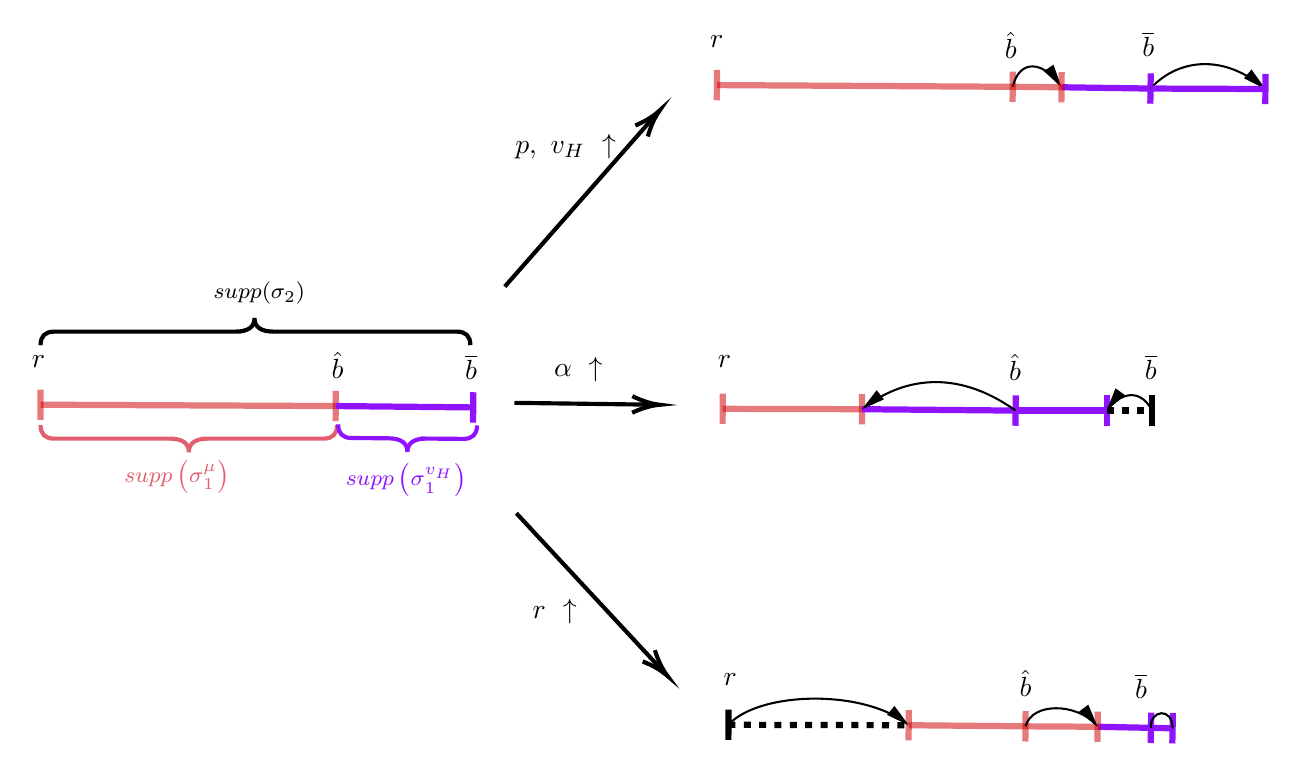
\begin{tikzpicture}[x=0.7pt,y=0.7pt,yscale=-1,xscale=1]

\draw [color={rgb, 255:red, 208; green, 2; blue, 5 }  ,draw opacity=0.53 ][line width=2.25]    (20.55,211.56) -- (172.9,212.26) ;
\draw [shift={(172.9,212.26)}, rotate = 180.26] [color={rgb, 255:red, 208; green, 2; blue, 5 }  ,draw opacity=0.53 ][line width=2.25]    (0,7.83) -- (0,-7.83)   ;
\draw [shift={(20.55,211.56)}, rotate = 180.26] [color={rgb, 255:red, 208; green, 2; blue, 5 }  ,draw opacity=0.53 ][line width=2.25]    (0,7.83) -- (0,-7.83)   ;
\draw [color={rgb, 255:red, 144; green, 19; blue, 254 }  ,draw opacity=1 ][line width=2.25]    (172.9,212.26) -- (243.89,212.96) ;
\draw [shift={(243.89,212.96)}, rotate = 180.57] [color={rgb, 255:red, 144; green, 19; blue, 254 }  ,draw opacity=1 ][line width=2.25]    (0,7.83) -- (0,-7.83)   ;
\draw  [color={rgb, 255:red, 208; green, 2; blue, 27 }  ,draw opacity=0.63 ][line width=1.5]  (20.55,222.07) .. controls (20.55,226.74) and (22.88,229.07) .. (27.55,229.07) -- (87.1,229.07) .. controls (93.77,229.07) and (97.1,231.4) .. (97.1,236.07) .. controls (97.1,231.4) and (100.43,229.07) .. (107.1,229.07)(104.1,229.07) -- (166.64,229.07) .. controls (171.31,229.07) and (173.64,226.74) .. (173.64,222.07) ;
\draw  [color={rgb, 255:red, 144; green, 19; blue, 254 }  ,draw opacity=1 ][line width=1.5]  (174.18,221.7) .. controls (174.15,226.37) and (176.46,228.72) .. (181.13,228.76) -- (199.97,228.9) .. controls (206.64,228.95) and (209.95,231.31) .. (209.92,235.98) .. controls (209.95,231.31) and (213.3,229) .. (219.97,229.05)(216.97,229.03) -- (238.82,229.2) .. controls (243.49,229.23) and (245.84,226.92) .. (245.87,222.25) ;
\draw  [line width=1.5]  (242.42,180.84) .. controls (242.42,176.17) and (240.09,173.84) .. (235.42,173.84) -- (141,173.84) .. controls (134.33,173.84) and (131,171.51) .. (131,166.84) .. controls (131,171.51) and (127.67,173.84) .. (121,173.84)(124,173.84) -- (27.55,173.84) .. controls (22.88,173.84) and (20.55,176.17) .. (20.55,180.84) ;
\draw [color={rgb, 255:red, 208; green, 2; blue, 5 }  ,draw opacity=0.53 ][line width=2.25]    (369.7,46.57) -- (522.38,47.46) ;
\draw [shift={(522.38,47.46)}, rotate = 180.34] [color={rgb, 255:red, 208; green, 2; blue, 5 }  ,draw opacity=0.53 ][line width=2.25]    (0,7.83) -- (0,-7.83)   ;
\draw [shift={(369.7,46.57)}, rotate = 180.34] [color={rgb, 255:red, 208; green, 2; blue, 5 }  ,draw opacity=0.53 ][line width=2.25]    (0,7.83) -- (0,-7.83)   ;
\draw [color={rgb, 255:red, 144; green, 19; blue, 254 }  ,draw opacity=1 ][line width=2.25]    (547.58,47.7) -- (593.54,48.36) ;
\draw [shift={(593.54,48.36)}, rotate = 180.81] [color={rgb, 255:red, 144; green, 19; blue, 254 }  ,draw opacity=1 ][line width=2.25]    (0,7.83) -- (0,-7.83)   ;
\draw    (522.38,47.46) .. controls (525.94,33.09) and (537.7,34.16) .. (546.5,46.15) ;
\draw [shift={(547.58,47.7)}, rotate = 236.48] [fill={rgb, 255:red, 0; green, 0; blue, 0 }  ][line width=0.08]  [draw opacity=0] (12,-3) -- (0,0) -- (12,3) -- cycle    ;
\draw    (593.54,48.36) .. controls (605.89,34.56) and (628.91,29.12) .. (651.45,47.45) ;
\draw [shift={(652.83,48.6)}, rotate = 220.6] [fill={rgb, 255:red, 0; green, 0; blue, 0 }  ][line width=0.08]  [draw opacity=0] (12,-3) -- (0,0) -- (12,3) -- cycle    ;
\draw [color={rgb, 255:red, 144; green, 19; blue, 254 }  ,draw opacity=1 ][line width=2.25]    (593.54,48.36) -- (652.83,48.6) ;
\draw [shift={(652.83,48.6)}, rotate = 180.24] [color={rgb, 255:red, 144; green, 19; blue, 254 }  ,draw opacity=1 ][line width=2.25]    (0,7.83) -- (0,-7.83)   ;
\draw [color={rgb, 255:red, 208; green, 2; blue, 5 }  ,draw opacity=0.53 ][line width=2.25]    (522.38,47.46) -- (547.58,47.7) ;
\draw [shift={(547.58,47.7)}, rotate = 180.56] [color={rgb, 255:red, 208; green, 2; blue, 5 }  ,draw opacity=0.53 ][line width=2.25]    (0,7.83) -- (0,-7.83)   ;
\draw [color={rgb, 255:red, 208; green, 2; blue, 5 }  ,draw opacity=0.53 ][line width=2.25]    (372.66,213.69) -- (444.61,213.88) ;
\draw [shift={(444.61,213.88)}, rotate = 180.16] [color={rgb, 255:red, 208; green, 2; blue, 5 }  ,draw opacity=0.53 ][line width=2.25]    (0,7.83) -- (0,-7.83)   ;
\draw [shift={(372.66,213.69)}, rotate = 180.16] [color={rgb, 255:red, 208; green, 2; blue, 5 }  ,draw opacity=0.53 ][line width=2.25]    (0,7.83) -- (0,-7.83)   ;
\draw [color={rgb, 255:red, 144; green, 19; blue, 254 }  ,draw opacity=1 ][line width=2.25]    (523.9,214.6) -- (570.89,214.6) ;
\draw [shift={(570.89,214.6)}, rotate = 180] [color={rgb, 255:red, 144; green, 19; blue, 254 }  ,draw opacity=1 ][line width=2.25]    (0,7.83) -- (0,-7.83)   ;
\draw [color={rgb, 255:red, 144; green, 19; blue, 254 }  ,draw opacity=1 ][line width=2.25]    (444.61,213.88) -- (523.9,214.6) ;
\draw [shift={(523.9,214.6)}, rotate = 180.52] [color={rgb, 255:red, 144; green, 19; blue, 254 }  ,draw opacity=1 ][line width=2.25]    (0,7.83) -- (0,-7.83)   ;
\draw [color={rgb, 255:red, 0; green, 0; blue, 0 }  ,draw opacity=1 ][line width=2.25]  [dash pattern={on 2.53pt off 3.02pt}]  (570.89,214.6) -- (594.38,214.6) ;
\draw [shift={(594.38,214.6)}, rotate = 180] [color={rgb, 255:red, 0; green, 0; blue, 0 }  ,draw opacity=1 ][line width=2.25]    (0,7.83) -- (0,-7.83)   ;
\draw    (523.9,214.6) .. controls (492.4,192.23) and (465.09,198.49) .. (446.06,212.77) ;
\draw [shift={(444.61,213.88)}, rotate = 321.74] [fill={rgb, 255:red, 0; green, 0; blue, 0 }  ][line width=0.08]  [draw opacity=0] (12,-3) -- (0,0) -- (12,3) -- cycle    ;
\draw    (594.38,214.6) .. controls (587.55,201.93) and (577.55,206.63) .. (572.05,213.11) ;
\draw [shift={(570.89,214.6)}, rotate = 305.64] [fill={rgb, 255:red, 0; green, 0; blue, 0 }  ][line width=0.08]  [draw opacity=0] (12,-3) -- (0,0) -- (12,3) -- cycle    ;
\draw [color={rgb, 255:red, 0; green, 0; blue, 0 }  ,draw opacity=1 ][line width=2.25]  [dash pattern={on 2.53pt off 3.02pt}]  (375.63,376.8) -- (468.69,377.01) ;
\draw [shift={(375.63,376.8)}, rotate = 180.13] [color={rgb, 255:red, 0; green, 0; blue, 0 }  ,draw opacity=1 ][line width=2.25]    (0,7.83) -- (0,-7.83)   ;
\draw [color={rgb, 255:red, 144; green, 19; blue, 254 }  ,draw opacity=1 ][line width=2.25]    (566.22,377.81) -- (593.76,378.38) ;
\draw [shift={(593.76,378.38)}, rotate = 181.2] [color={rgb, 255:red, 144; green, 19; blue, 254 }  ,draw opacity=1 ][line width=2.25]    (0,7.83) -- (0,-7.83)   ;
\draw [color={rgb, 255:red, 208; green, 2; blue, 5 }  ,draw opacity=0.53 ][line width=2.25]    (468.69,377.01) -- (528.99,377.59) ;
\draw [shift={(528.99,377.59)}, rotate = 180.55] [color={rgb, 255:red, 208; green, 2; blue, 5 }  ,draw opacity=0.53 ][line width=2.25]    (0,7.83) -- (0,-7.83)   ;
\draw [shift={(468.69,377.01)}, rotate = 180.55] [color={rgb, 255:red, 208; green, 2; blue, 5 }  ,draw opacity=0.53 ][line width=2.25]    (0,7.83) -- (0,-7.83)   ;
\draw [color={rgb, 255:red, 208; green, 2; blue, 5 }  ,draw opacity=0.53 ][line width=2.25]    (528.99,377.59) -- (566.22,377.81) ;
\draw [shift={(566.22,377.81)}, rotate = 180.33] [color={rgb, 255:red, 208; green, 2; blue, 5 }  ,draw opacity=0.53 ][line width=2.25]    (0,7.83) -- (0,-7.83)   ;
\draw [color={rgb, 255:red, 144; green, 19; blue, 254 }  ,draw opacity=1 ][line width=2.25]    (593.76,378.38) -- (604.93,378.6) ;
\draw [shift={(604.93,378.6)}, rotate = 181.11] [color={rgb, 255:red, 144; green, 19; blue, 254 }  ,draw opacity=1 ][line width=2.25]    (0,7.83) -- (0,-7.83)   ;
\draw    (375.63,376.8) .. controls (390.96,359.9) and (443.46,358.04) .. (467.27,375.89) ;
\draw [shift={(468.69,377.01)}, rotate = 219.53] [fill={rgb, 255:red, 0; green, 0; blue, 0 }  ][line width=0.08]  [draw opacity=0] (12,-3) -- (0,0) -- (12,3) -- cycle    ;
\draw    (528.99,377.59) .. controls (532.57,364.85) and (555.35,365.8) .. (565.07,376.43) ;
\draw [shift={(566.22,377.81)}, rotate = 233.11] [fill={rgb, 255:red, 0; green, 0; blue, 0 }  ][line width=0.08]  [draw opacity=0] (12,-3) -- (0,0) -- (12,3) -- cycle    ;
\draw    (593.76,378.38) .. controls (593.02,369.08) and (604.93,367.49) .. (604.93,378.6) ;
\draw [line width=1.5]    (338.22,61.85) -- (260.2,150.6) ;
\draw [shift={(340.2,59.6)}, rotate = 131.32] [color={rgb, 255:red, 0; green, 0; blue, 0 }  ][line width=1.5]    (14.21,-4.28) .. controls (9.04,-1.82) and (4.3,-0.39) .. (0,0) .. controls (4.3,0.39) and (9.04,1.82) .. (14.21,4.28)   ;
\draw [line width=1.5]    (337.2,211.56) -- (265.2,210.6) ;
\draw [shift={(340.2,211.6)}, rotate = 180.76] [color={rgb, 255:red, 0; green, 0; blue, 0 }  ][line width=1.5]    (14.21,-4.28) .. controls (9.04,-1.82) and (4.3,-0.39) .. (0,0) .. controls (4.3,0.39) and (9.04,1.82) .. (14.21,4.28)   ;
\draw [line width=1.5]    (342.16,349.4) -- (266.2,267.6) ;
\draw [shift={(344.2,351.6)}, rotate = 227.12] [color={rgb, 255:red, 0; green, 0; blue, 0 }  ][line width=1.5]    (14.21,-4.28) .. controls (9.04,-1.82) and (4.3,-0.39) .. (0,0) .. controls (4.3,0.39) and (9.04,1.82) .. (14.21,4.28)   ;

\draw (14.44,184.47) node [anchor=north west][inner sep=0.75pt]    {$r$};
\draw (169.26,182.91) node [anchor=north west][inner sep=0.75pt]    {$\hat{b}$};
\draw (238.11,184.42) node [anchor=north west][inner sep=0.75pt]    {$\overline{b}$};
\draw (62.17,238.54) node [anchor=north west][inner sep=0.75pt]  [font=\footnotesize,color={rgb, 255:red, 208; green, 2; blue, 27 }  ,opacity=0.63 ]  {$supp\left( \sigma {_{1}^{\mu}}\right)$};
\draw (176.53,240.42) node [anchor=north west][inner sep=0.75pt]  [font=\footnotesize,color={rgb, 255:red, 144; green, 19; blue, 254 }  ,opacity=1 ]  {$supp\left( \sigma {_{1}^{v_H}}\right)$};
\draw (108.28,146.79) node [anchor=north west][inner sep=0.75pt]  [font=\footnotesize,color={rgb, 255:red, 0; green, 0; blue, 0 }  ,opacity=1 ]  {$supp( \sigma _{2})$};
\draw (364.59,19.17) node [anchor=north west][inner sep=0.75pt]    {$r$};
\draw (516.74,17.47) node [anchor=north west][inner sep=0.75pt]    {$\hat{b}$};
\draw (587.75,17.67) node [anchor=north west][inner sep=0.75pt]    {$\overline{b}$};
\draw (589.06,184.37) node [anchor=north west][inner sep=0.75pt]    {$\overline{b}$};
\draw (518.99,183.81) node [anchor=north west][inner sep=0.75pt]    {$\hat{b}$};
\draw (368.54,184.79) node [anchor=north west][inner sep=0.75pt]    {$r$};
\draw (371.53,348.65) node [anchor=north west][inner sep=0.75pt]    {$r$};
\draw (524.35,347.03) node [anchor=north west][inner sep=0.75pt]    {$\hat{b}$};
\draw (583.98,348.87) node [anchor=north west][inner sep=0.75pt]    {$\overline{b}$};
\draw (264,70.4) node [anchor=north west][inner sep=0.75pt]    {$p, \ v_H\ \uparrow $};
\draw (284,185.4) node [anchor=north west][inner sep=0.75pt]    {$\alpha \ \uparrow $};
\draw (273,310.4) node [anchor=north west][inner sep=0.75pt]    {$r \ \uparrow $};

\end{tikzpicture}

\noindent Above is a graphical representation of the result. Intuitively, as $ p $ and $ c $ increase the ad slot gets more valuable, inducing DSPs to start playing higher bids. More precisely, the upper bounds of $ supp( \sigma_1^{\mu^*} ) $ and $ supp\left( \sigma_2^* \right) $ move to the right, whereas both the lower bound and the upper bound of $ supp\left( \sigma_1^{v_H^*} \right) $ shift to the right: conditional on being type $ t_1 = v_H $, $ d_1 $ not only starts playing higher bids but she also stops submitting relatively low bids. When $ \alpha $ increases, i.e. when $ d_1 $ gets access to user preferences more frequently, both $ d_1 $ and $ d_2 $ start submitting lower bids. Finally, when the floor price $ r $ increases, DSPs are forced to stop submitting low bids, and at the same time they start including slightly higher bids in their supports. In order to understand more thoroughly how fundamental parameters shape bidding behavior, we perform comparative statics on the equilibrium distributions.

\begin{cor}
Let $ \left( F_1^{v_H^*},\ F_1^{\mu^*},\ F_2^*  \right) $ be the equilibrium C.D.F. characterized above. Then:

\begin{itemize}
    \item[1.] $ F_1^{v_H^*},\ F_1^{\mu^*},\ F_2^* $ are decreasing in $ p $, in $ v_H $ and in $ r $;

    

    \item[2.] $ F_1^{v_H^*},\ F_1^{\mu^*},\ F_2^* $ are increasing in $ \alpha $.
\end{itemize}

\end{cor}

\noindent Combining our comparative statics results, we conclude that both DSPs play more aggressively if either the value of the ad slot or the floor price increase. Indeed, DSPs not only include increasingly higher bids in their supports, but they also redistribute mass from low bids to high bids. As a consequence, competition is intensified. An increase in $ \alpha $ instead relaxes competition. This follows directly from the fact that all equilibrium CDFs are increasing in $ \alpha $. Additionally, both DSPs shrink their supports and shift mass from high bids to low bids, further reinforcing this competitive softening effect. \par

\noindent The economic intuition behind this result is as follows. First, if $ d_1 $ gets access to user preferences more frequently, the probability that she acknowledges the ad slot to be worthless for her increases. In this state of the world, $ d_1 $ drops from the auction and the best reply for $ d_2 $ is to bid the lowest acceptable bid. Therefore, $ d_2 $ has incentives to move mass from relatively high bids towards the floor price $ r $. Secondly, as $ d_2 $ shifts mass away from high bids, also $ d_1 $ has incentives to emulate her opponent, in order to soften competition and increase the profit margin in case of a win. Overall, these comparative statics reflect the strategic complementarity of bids in first-price auctions. \par

\subsubsection{Revenues}

\noindent Let us determine the equilibrium revenues of $ d_1, d_2 $ and compare the two in order to quantify the impact of asymmetric information.

\begin{cor}\label{revenues-comparative}
The equilibrium expected revenues of $ d_1, d_2 $ are:

\begin{align*}
 R_1 (p, v_H, \alpha, r) &= \frac{\alpha (1 - p)\left[ v_H+ \alpha (\mu - r) \right] \left[ p(v_H - \alpha r) + (1 - \alpha)(\mu - r) \right]}{v_H - \alpha r} \\[5pt]
 R_2(p, v_H, \alpha, r) &= \alpha (1 - p) (\mu - r)
\end{align*}

\noindent Moreover, we have that:
\begin{itemize}
    \item[-] $ R_1 > R_2 $ \ for all parameter values.

    

    \item[-] $ R_i $ is increasing in $ c $ and in $ \alpha $ for $ i = 1,2 $.

    

    \item[-] $ R_i $ is concave in $ p $ for $ i = 1,2 $.

    

    \item[-] $ R_i $ is decreasing in $ r $ for $ i = 1,2 $.

    

    \item[-] Define $\tilde{r} := \frac{v_H}{2}\left[(1+p) - \sqrt{1+p^2}\right]$. The informational revenue gap $R_1 - R_2$ is hump-shaped in $\alpha$ if $r < \tilde{r}$: it achieves a unique interior maximum at some $\tilde{\alpha} \in (0,1)$ and is strictly decreasing on $(\tilde{\alpha}, 1]$. If $r \geq \tilde{r}$, the informational revenue gap is monotonically increasing in $\alpha$.
\end{itemize}
\end{cor}

\noindent The last property follows from a structural feature of $R_1$ that will also play a central role in the data licensing analysis of Section~\ref{licensing}.

\begin{lem}\label{R1-properties}
    The revenue function $R_1$ is increasing in $\alpha$ and such that it changes concavity at most once: it is either concave throughout, or convex for low values of $\alpha$ and then concave.
\end{lem}

\noindent The proof is available in the Appendix. Lemma~\ref{R1-properties} establishes that the competition-softening mechanism exhibits diminishing returns: $R_1$ is eventually concave in $\alpha$, and once the marginal return to information access begins to decline, the decline only deepens. Combined with the linearity of $R_2$ in $\alpha$, this is what drives the last property of the Corollary: $R_2$ grows at the constant rate $(1-p)(\mu - r)$ per unit of $\alpha$, while $R_1$'s growth rate is eventually decreasing. When the floor price is below $\tilde{r}$, the constant-rate growth of $R_2$ eventually overtakes the decelerating growth of $R_1$, so the gap peaks in the interior and then narrows. Figure~\ref{revenues-plot}(a) illustrates these patterns.

\begin{figure}[h]
    \centering
    \begin{subfigure}[b]{0.45\textwidth}
        \centering
        \begin{tikzpicture}
\begin{axis}[
    width=\linewidth,
    height=0.8\linewidth,
    xlabel={$\alpha$},
    xmin=0, xmax=1,
    ymin=0,
    xtick={0,1},
    ytick=\empty,
    axis lines=left,
    axis line style={-},
    xlabel style={at={(ticklabel* cs:1)}, anchor=west},
    clip=false,
    samples=100,
    domain=0:1,
    smooth,
]

\pgfmathsetmacro{\vH}{2}
\pgfmathsetmacro{\muval}{1}
\pgfmathsetmacro{\rval}{0.2}
\pgfmathsetmacro{\pval}{0.5}

\addplot[violet, very thick] {
    (x * (1-\pval) * (\vH + x*(\muval-\rval)) * (\pval*(\vH - x*\rval) + (1-x)*(\muval-\rval))) / (\vH - x*\rval)
} node[pos=0.85, above left, violet] {$\Pi_1$};

\addplot[black, very thick] {
    x * (1-\pval) * (\muval - \rval)
} node[pos=0.85, below right, black] {$\Pi_2$};

\end{axis}
\end{tikzpicture}
         \caption{Equilibrium revenues vs.\ $ \alpha $.}
    \end{subfigure}
    \hfill
    \begin{subfigure}[b]{0.45\textwidth}
        \centering
        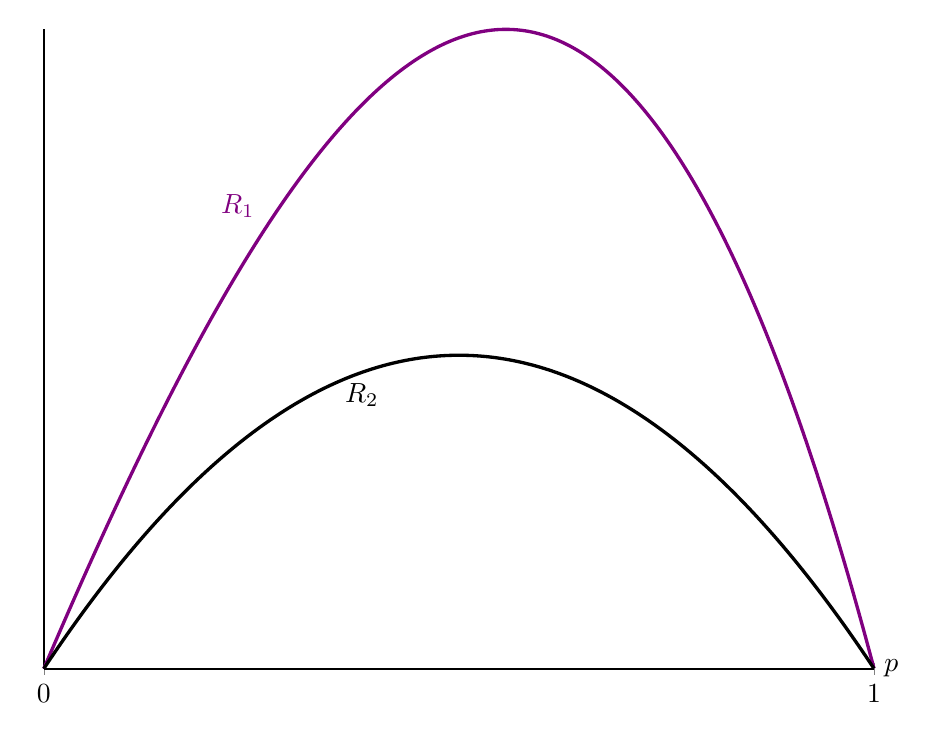
\begin{tikzpicture}
\begin{axis}[
    width=\linewidth,
    height=0.8\linewidth,
    xlabel={$p$},
    xmin=0, xmax=1,
    ymin=0,
    xtick={0,1},
    ytick=\empty,
    axis lines=left,
    axis line style={-},
    xlabel style={at={(ticklabel* cs:1)}, anchor=west},
    clip=false,
    samples=100,
    domain=0:1,
    smooth,
]

\pgfmathsetmacro{\vH}{2}
\pgfmathsetmacro{\rratio}{0.2}  \pgfmathsetmacro{\alphaval}{0.7}

\addplot[violet, very thick] {
    (\alphaval * (1-x) * (\vH + \alphaval*x*\vH*(1-\rratio)) * (x*(\vH - \alphaval*\rratio*x*\vH) + (1-\alphaval)*x*\vH*(1-\rratio))) / (\vH - \alphaval*\rratio*x*\vH)
} node[pos=0.3, above left, violet] {$R_1$};

\addplot[black, very thick] {
    \alphaval * (1-x) * x * \vH * (1-\rratio)
} node[pos=0.4, below, black] {$R_2$};

\end{axis}
\end{tikzpicture}
         \caption{Equilibrium revenues vs.\ $ p $.}
    \end{subfigure}
    \caption{Equilibrium revenues as functions of $ \alpha $ and $ p $.}
    \label{revenues-plot}
\end{figure}

\noindent As expected, preferential access to user data significantly benefits $ d_1 $. There are two notable features to highlight. First, as $ d_1 $ gains more frequent access to data, not only does $ d_1 $ benefit from increased revenues, but $ d_2 $ also experiences a revenue boost. This is a direct consequence of softened competition, as we pointed out in the previous comparative statics analysis. Second, revenues are maximized when $ p $ takes on intermediate values, corresponding to cases where there is greater uncertainty about consumer preferences. When $ p $ is extremely low, consumers rarely click on the displayed ads, resulting in low revenue. When $ p $ is extremely high, the strong likelihood of monetizing a click triggers intense competition, prompting both DSPs to bid aggressively and reducing their profit margins. At intermediate values of $ p $, competition is less fierce, allowing both DSPs to earn higher revenues.

\noindent That both DSPs benefit from increased $\alpha$ is a direct consequence of the competition softening described above. One might wonder, however, why this effect is not offset by the fact that higher $\alpha$ also means $d_1$ observes $v_H$ more frequently, seemingly intensifying competition in those states. The resolution lies in the structure of $d_2$'s guaranteed payoff. Since $d_2$ does not observe $d_1$'s type realization, she selects a strategy against the ex-ante mixture of opponent types. Regardless of the equilibrium, $d_2$ can guarantee herself a payoff of at least $\alpha(1-p)(\mu - r)$ by adopting the strategy of always bidding $r$: she wins whenever $d_1$ is absent and earns the full surplus $(\mu - r)$ in expectation, and otherwise loses the auction and earns zero. This guaranteed payoff depends only on the probability mass in the favorable tail of $d_1$'s type distribution and is completely insulated from the unfavorable tail, because auction profits are bounded below by zero. In formal terms, $d_2$'s profit from bidding $r$ takes the form $(\mu - r) \cdot \mathbf{1}\{v_1 < r\}$: it is positive when $d_1$ draws a low value and drops out, and zero otherwise. Increasing $\alpha$ is a mean-preserving spread on $d_1$'s valuation: the unconditional expectation $\alpha p v_H + (1-\alpha)\mu = \mu$ is invariant in $\alpha$. The spread fattens both tails, but only the favorable tail (more frequent dropout) affects $d_2$'s guaranteed payoff, while the unfavorable tail ($d_1$ observing $v_H$) imposes no additional cost. In equilibrium, the indifference condition across $d_2$'s bidding support pins her expected revenue exactly to the floor-price payoff: $R_2 = \alpha(1-p)(\mu - r)$. The fiercer competition in $v_H$-states is thus fully absorbed by the equilibrium bid adjustment, while the gains from more frequent dropout are captured entirely at the lower bound of the support.

\noindent The structure of $d_2$'s guaranteed payoff is also the key to understanding the Lemma and the behaviour of the informational revenue gap $R_1 - R_2$. Write $R_1 = \alpha \cdot \rho(\alpha)$, where $\rho(\alpha)$ is the revenue gain that $d_1$ extracts per unit of information access. Each marginal unit of $\alpha$ converts an uninformed event---in which symmetric competition dissipates all bidder surplus---into an informed event in which $d_1$ can selectively participate. But the revenue gain per informed event, $\rho(\alpha)$, is itself a function of $\alpha$ through the equilibrium bidding adjustment: at high $\alpha$, $d_2$ has already shifted most of her bidding mass toward the floor price, so the marginal informed event faces a pre-adjusted opponent and generates less incremental surplus. In formal terms, the third derivative of $R_1$ with respect to $\alpha$ is non-positive (as shown in the Appendix), ensuring that once diminishing returns set in, the decline in the marginal revenue gain can accelerate but never reverse.

\noindent While both revenues are increasing in $\alpha$, the \emph{gap} $R_1 - R_2$ need not be monotone. Two forces compete as $\alpha$ rises. The first is the direct revenue advantage created by selective participation: each additional informed event lets $d_1$ avoid low-value auctions and thus pushes the gap upward. This force dominates at low $\alpha$, where $d_2$ has not yet adapted her bidding to the presence of an informed opponent. The second is \emph{gap compression}: $R_2 = \alpha(1-p)(\mu - r)$ grows at the constant rate $(1-p)(\mu - r)$ per unit of $\alpha$, because each dropout event yields $d_2$ the full surplus $(\mu - r)$ at the floor price. By Lemma~\ref{R1-properties}, $R_1$ is eventually concave, so its growth rate is eventually decreasing. When the floor price is sufficiently low ($r < \tilde{r}$), the constant-rate accrual of dropout surplus to $d_2$ eventually outpaces the decelerating growth of $R_1$, and the gap narrows.

\noindent The floor price governs the relative strength of the two forces through the surplus term $(\mu - r)$, captured by $d_2$ each time $d_1$ drops out. When $r$ is low, this surplus is large: the linear force is strong and the gap peaks in the interior. When $r$ approaches $\mu$, the dropout surplus vanishes, the linear force weakens, and $d_1$'s direct revenue advantage dominates throughout. The threshold $\tilde{r} = \frac{v_H}{2}\left[(1+p) - \sqrt{1+p^2}\right]$ marks the exact boundary.

\subsubsection{Engagement Rates}

\noindent In our framework, consumer engagement with the displayed ad is the measure of campaign success and a proxy for advertiser welfare. Under the baseline click-campaign interpretation (without loss of generality), this reduces to click rates. Engagement rates for the product served by $d_1$ or $d_2$ read respectively
\begin{align*}
    \mathbb{P} (\text{product} \ 1 \ \text{is clicked}) =& p \left[  \alpha \mathbb{P}(d_1 \ \text{wins}\ | \ t_1 = v_H) + (1-\alpha)  \mathbb{P}(d_1 \ \text{wins}\ | \ t_1 = \mu) \right] \\[5pt]
    \mathbb{P} (\text{product} \ 2 \ \text{is clicked}) =& p \left[ \alpha (1 - p) + \alpha p \mathbb{P}(d_2 \ \textrm{wins} \ | \ t_1 = v_H) + (1 - \alpha) \mathbb{P}(d_2 \ \textrm{wins} \ | \ t_1 = \mu)  \right].
\end{align*}

\noindent Winning probabilities are computed in the Appendix. From a graphical inspection, we can observe that the engagement rate for $d_2$ is maximised either at $\alpha = 0$ or at $\alpha = 1$, depending on the value of $p$. In particular, for $p \leq \hat{p} \approx 0.6$, engagement rates are maximised at $\alpha = 1$, which is to say that the advertiser served by the uninformed platform prefers maximal information asymmetry when it is relatively unlikely that the object has a positive value. The key force stems from the fact that at low $p$, $d_2$ wins relatively more often against an opponent who observes that its object is worthless. In the two edge cases,
\begin{align*}
    \mathbb{P}(\text{product} \ 2 \ \text{is clicked}) = \begin{cases}
        p \,  \mathbb{P}(d_2 \ \textrm{wins} \ | \ t_1 = \mu),  & \alpha = 0; \\[5pt]
        p \left[(1 - p) + p \mathbb{P}(d_2 \ \textrm{wins} \ | \ t_1 = v_H)  \right], & \alpha = 1.
    \end{cases}
\end{align*}

\noindent Graphically, we observe that
\begin{align*}
    \underbrace{(1 - p) + p \mathbb{P}(d_2 \ \textrm{wins} \ | \ t_1 = v_H, \, \alpha = 1)}_{\mathbb{P}(d_2 \ \textrm{wins} \ | \ \alpha = 1)} \begin{cases}
        > \mathbb{P}(d_2 \ \textrm{wins} \ | \ t_1 = \mu, \, \alpha = 0), & p < \hat{b} \\[5pt]
        < \mathbb{P}(d_2 \ \textrm{wins} \ | \ t_1 = \mu,\, \alpha = 0), & p > \hat{b}.
    \end{cases}
\end{align*}

\noindent Given that for any $p$, $\mathbb{P}(d_2 \ \textrm{wins} \ | \ t_1 = \mu, \, \alpha = 0)>p \mathbb{P}(d_2 \ \textrm{wins} \ | \ t_1 = v_H, \, \alpha = 1)$, we can conclude that the non-monotonicity is entirely driven by the term $1-p$, which represents the winning probability for $d_2$ conditional on $d_1$ having observed $v_1 = 0$. To summarise the intuition: if the object is not very likely to have value, the winning gain resulting by outbidding the informed $d_1$ with a worthless object is such that the advertiser served by the uninformed platform prefers that information asymmetries are maximised, i.e. that $d_1$ observes the value of the object with probability 1. \par

\noindent It can further be observed that $\mathbb{P}(\text{product} \ 2 \ \text{is clicked})$ is minimised at an interior $\alpha \in (0,1)$, for any value of $p$. As a dual, $\mathbb{P}(\text{product} \ 1 \ \text{is clicked})$ is maximised at an interior $\alpha \in (0,1)$, for any value of $p$.  \par

\noindent A stark result is that the engagement rate for product $1$ is strictly larger than the engagement rate for product $2$, for any $\alpha > 0$. In other words, an arbitrarily small informational advantage is sufficient to prevent two advertisers promoting minimally heterogeneous products from single-homing in two different DSPs. The natural segmentation observed in the demand-side market cannot be reproduced in our simple setting. In extension \ref{multiple-ADV}, we show that segmentation can be recovered by having DSPs serve heterogeneous masses of ex-ante identical advertisers. As long as information asymmetries are not absolute, if $\alpha < 1$, congestion effects eventually dominate information dominance.

We now study how information affects the probability that the displayed ad generates the high value $ v_H $. This object provides a natural measure of allocative performance: it captures the probability that the impression is assigned to an advertiser for whom the consumer is valuable. Let $ E $ denote the event that the equilibrium displayed ad generates value $ v_H $. Since $ d_1 $ is uninformed with probability $ 1-\alpha $, in which case $ t_1 = \mu $, and informed with probability $ \alpha $, we can write
\begin{equation}\label{HP}\tag{HP}
\mathbb{P}(E)
=
(1 - \alpha)\mathbb{P}(E \mid t_1 = \mu)
+
\alpha \mathbb{P}(E \mid d_1 \text{ informed}).
\end{equation}

\noindent We compute the two conditional probabilities separately. First, suppose $ t_1 = \mu $ and let
\[
\pi_\mu:=\Pr(d_1\text{ wins}\mid t_1=\mu)
\]
The value of $\pi_\mu$ is determined by equilibrium play and in particular it depends on $ \alpha $. However, conditional on $ t_1 = \mu $, neither bidder's strategy is contingent on the realized pair $ (v_1,v_2) $. Thus, the auction does not select the winner on the basis of realized match quality. Formally,
\begin{align*}
\mathbb{P}(E \mid t_1 = \mu)
&=
\mathbb{P}(v_1=v_H,v_2=v_H) \\
&\quad+
\mathbb{P}(v_1=v_H,v_2=v_L)\mathbb{P}(d_1\text{ wins}\mid t_1=\mu) \\
&\quad+
\mathbb{P}(v_1=v_L,v_2=v_H)\mathbb{P}(d_2\text{ wins}\mid t_1=\mu) \\
&=
p^2+p(1-p)\pi_\mu+p(1-p)(1-\pi_\mu) \\
&=p.
\end{align*}

\noindent The intuition is that, when $ t_1 = \mu $, the auction is equivalent to choosing between two boxes. Each box contains a high-value ad with probability $ p $. Equilibrium bidding leads the mechanism to choose box $ 1 $ with probability $ \pi_\mu $ and box $ 2 $ with probability $ 1 - \pi_\mu $, but since the selection rule is not based on the contents of the boxes, the selected box contains a high-value ad with probability exactly $ p $. Therefore, equilibrium mixing determines which DSP wins the auction, but it does not affect the probability that the winner obtains high value.

Now consider the states in which $ d_1 $ is informed. In this case, the allocation becomes correlated with realized values. There are three relevant value profiles to consider. If $ (v_1,v_2) = (v_H,v_H) $, then the displayed ad generates value $v_H$ regardless of which DSP wins. If $(v_1,v_2)=(v_L,v_H)$, then $d_1$ observes $v_L<r$ and does not participate, so $d_2$ wins and the displayed ad again generates value $v_H$. The total probability of these two events is
\[
p^2+(1-p)p=p.
\]

\noindent If $ (v_1,v_2) = (v_H,v_L) $, which occurs with probability $ p(1-p) $, a high-value ad is displayed if and only if $ d_1 $ wins the auction. Let
\[
P_H(\alpha):=\mathbb{P}(d_1\text{ wins} \mid t_1=v_H)
\]

\noindent Then,
\begin{align*}
\Pr(E\mid d_1\text{ informed})
&=
p+p(1-p)P_H(\alpha).
\end{align*}

\noindent Substituting the two conditional probabilities into \eqref{HP} we get
\begin{align*}
\Pr(E)
&=
(1-\alpha)\mathbb{P}(E \mid t_1=\mu)
+
\alpha\mathbb{P}(E\mid d_1\text{ informed}) \\
&=
(1-\alpha)p+\alpha\left[p+p(1-p)P_H(\alpha)\right] \\
&=
p+\alpha p(1-p)P_H(\alpha).
\end{align*}
This expression separates a targeting-free benchmark from the incremental gain generated by information. The first term, $p$, is the probability that the displayed ad generates value $v_H$ absent targeting from $d_1$'s information. The second term,
\[
\alpha p(1-p)P_H(\alpha)
\]
is the gain from targeting. Information matters only through this term, and it creates value in the asymmetric state $(v_1,v_2)=(v_H,v_L)$, where the high-value bidder is $d_1$ and the low-value bidder is $d_2$. The comparative statics with respect to $\alpha$ can therefore be understood through an extensive and an intensive margin. Differentiating the targeting gain yields
\[
\frac{d}{d\alpha}\left[\alpha p(1-p)P_H(\alpha)\right]
=
p(1-p)
\left[
\underbrace{P_H(\alpha)}_{\text{extensive margin}}
+
\underbrace{\alpha P_H'(\alpha)}_{\text{intensive margin}}
\right].
\]

\noindent The extensive margin is positive: as $ \alpha $ increases, states in which $ d_1 $ observes that it is a high-value bidder occurs more often. The intensive margin captures how $ d_1 $'s equilibrium winning probability changes with $ \alpha $. Using our closed-form expressions, we can show that $ P_H'(\alpha) < 0 $: \textbf{conditional on observing $ v_H $, $ d_1 $ shades more aggressively as competition softens, and therefore wins less often}. Hence the total probability that a high-value ad is displayed in equilibrium increases with $ \alpha $ whenever the extensive-margin gain from more frequent information dominates the intensive-margin loss from the lower conditional winning probability of the high type. We can show that, in our framework
\[
P_H(\alpha) + \alpha P_H'(\alpha) > 0  \forall (\alpha, p, v_H, r)
\]

\noindent Thus, increased access to asymmetric information improves targeting overall.

\section{Data-Sharing Remedies}\label{sec:data-sharing}\label{licensing}

\noindent We now turn to analyse a specific data-sharing remedy that has featured prominently in recent regulatory discussions: requiring the vertically integrated platform to grant its competitor direct access to consumer preference data. The underlying rationale is straightforward: the integrated entity cannot be made to ``forget'' information it has already acquired through its ad server, since information asymmetries are pervasive and the identity of consumers cannot be linked \textit{ex ante} to how relevant each of them might be for advertisers served by competing DSPs. A regulator can, however, mandate that the integrated platform share consumer identification data with rival DSPs whenever it observes consumer preferences, thereby levelling the playing field on the demand side. We treat this open-infrastructure regime as a natural benchmark.\footnote{This benchmark is closely related in spirit to the bidder-optimal information design problem studied by \textcite{bergemannBidderOptimalInformationStructures2024}, but our general disclosure problem does not admit the same reduction. Under hard evidence, $d_1$ can only send truthful certifications of realised values, while the uninformed type cannot generate state-contingent messages; continuation payoffs therefore depend not only on a posterior mean, but on the composition of the induced first-price subgame. The problem thus does not collapse to a convex one-dimensional posterior design problem.} Furthermore, we allow for data sharing to be monetised by the integrated entity through a licensing fee. Note that requiring $d_1$ to share \textit{all} of its private information (both $v_1$ and $v_2$) would lead to symmetric perfect information and trivial Bertrand competition at the reserve price; a more natural intervention targets the competitor's relevant signal only, namely $v_2$. Formally, we study the regime in which $d_1$ provides $d_2$ with access to the realisation of $v_2$ at price $\phi \geq 0$ whenever $d_1$ observes $(v_1, v_2)$, while $d_1$ retains its private knowledge of $v_1$. This captures the essential feature of data portability mandates and interoperability requirements that have been proposed by the \textcite{competitionandmarketsauthorityOnlinePlatformsDigital2020}: an architectural commitment to open the integrated platform's consumer data infrastructure to competitors.\par

\noindent Under the mandated sharing regime, whenever $ d_1 $ is informed, $ d_2 $ learns $v_2$ and can avoid bidding for worthless impressions. However, $ d_2 $ still faces uncertainty about whether $ d_1 $ will compete when $v_2 = v_H$, as $ d_2 $ does not observe $v_1$. Total revenues for the two firms can be decomposed as follows:
\begin{itemize}
    \item Suppose that $d_1$ is uninformed about $v_2$; then both bidders know that they compete for a slot of expected value $\mu$, and earn zero expected profits.
    \item Suppose that $d_1$ observes $v_2$; three possible cases arise:
    \begin{enumerate}
        \item $v_1 = v_2 = v_L$. Neither firm bids, expected revenues are zero.
        \item $v_1 = v_H$, $v_2 = v_L$. $d_1$ bids $r$ while $d_2$ stays out of the auction. This event has probability $\alpha p (1-p)$.
        \item $v_2 = v_H$, $v_1$ unknown. A new auction with imperfect information takes place. We derive equilibrium bidding functions for this subgame below.
    \end{enumerate}
\end{itemize}

\noindent We construct an equilibrium in mixed strategies. The two indifference conditions are
\begin{align*}
    (v_H-b)F_2^{\ell}(b) = \kappa_1 \\[5pt]
    (v_H-b)\left[pF_1^{\ell}(b) + 1-p \right] = \kappa_2
\end{align*}
where $F_1^{\ell}$, $F_2^{\ell}$ are bidding functions of $d_1$ and $d_2$ respectively under the data licensing regime, where $F_1^{\ell}$ is played if and only if $v_1 = v_H$. We derive equilibrium distributions following the same logic as in the main analysis. \par

\noindent The supports of $F_1^{\ell}$ and $F_2^{\ell}$ coincide for the usual reasons outlined in the previous section; moreover, $d_2$ places positive mass on the lower bound $\underline{b}^\ell = r$. To derive the upper bound of the support and equilibrium distributions, we use $F_1^{\ell}(r) = 0$. We get that $\kappa_2 = (v_H-r)(1-p)$, implying that
\begin{equation*}
    F_1^{\ell *}(b) = \frac{1-p}{p} \left( \frac{b-r}{v_H-b} \right).
\end{equation*}
We back out $\bar{b}^\ell$ by setting $ F_1^{\ell}(\bar{b}^\ell) = 1$:
\begin{equation*}
    \bar{b}^\ell = \mu+(1-p)r.
\end{equation*}
This in turn allows us to solve for $\kappa_1$ and $F_2^{\ell *}$:
\begin{equation*}
    \kappa_1 = v_H- \bar{b}^\ell = (v_H-r)(1-p).
\end{equation*}
Note that $\kappa_1 = \kappa_2$. Finally,
\begin{equation*}
    F_2^{\ell *}(b) = (1-p)\left(\frac{v_H-r}{v_H-b}\right).
\end{equation*}
One can note that the point mass conjecture for $F_2^{\ell *}$ holds: $F_2^{\ell *}(r) = 1-p$, i.e. $d_2$ puts on $b = r$ exactly the same mass corresponding to the probability that $d_1$ draws $v_1 = 0$. \par

\noindent Note that expected revenues for both bidders under this scenario is $(v_H-r)(1-p)$. Summing all terms up, we get expected revenues
\begin{equation*}
    R_2^\ell = \alpha p (v_H-r)(1-p).
\end{equation*}

\noindent A natural first question is whether $d_1$ would ever share consumer data voluntarily, absent regulatory intervention. Under the mandated sharing regime without compensation, $d_1$'s profits are $R_1^s = \alpha p (1-p^2)(v_H-r)$. It can be shown that uncompensated sharing always makes $d_1$ strictly worse off:
\begin{lem}\label{no-sharing}
    $R_1 - R_1^s \geq0$ for all parameter values.
\end{lem}

\noindent The result follows from simple algebraic manipulation and confirms that data sharing must be imposed by a regulator; the platform's private incentives always favour the closed ecosystem when sharing is uncompensated. Having established this, we ask whether $d_1$ can at least \textit{monetise} the forced data access: if the regulator mandates that $d_1$ open its infrastructure to $d_2$, could $d_1$ offset its competitive losses by charging a licensing fee? To compute an upper bound on $d_1$'s monetisation potential, we assume $d_1$ can make a take-it-or-leave-it offer to $d_2$, thereby extracting $d_2$'s full willingness to pay. By subtracting $R_2$ from $R_2^\ell$, we obtain $d_2$'s willingness to pay for data access, $R_2^\ell - R_2 = \alpha(1-p)^2r$. Total revenues under data licensing for $d_1$ are therefore
\begin{equation*}
     R_1^\ell = \alpha p (1-p)(v_H-r) + \alpha p^2 (1-p)(v_H-r) + \alpha(1-p)^2r = \alpha p (1-p^2)(v_H-r) + \alpha(1-p)^2r.
\end{equation*}
This tells us that $R_1^\ell > R_2^\ell$.

\noindent The two revenue functions of interest have the following feature: $R_1^\ell$ is linear increasing in $\alpha$, while $R_1$ is increasing and changes concavity at most once (Lemma~\ref{R1-properties}). These two properties allow us to provide tight bounds on the parameters under which the mandated remedy imposes a net cost on $d_1$, even when the platform can fully monetise data access. Our main result is that for a range of parameters capturing plausible market conditions, the competitive advantage from proprietary data exceeds the maximal licensing revenue. To build intuition, we first illustrate two boundary conditions on the floor price and a special case of the main result for high engagement probabilities. \par

\noindent Define the net surplus from the closed ecosystem as $\Delta := R_1 - R_1^\ell$. A first straightforward result is that if the floor price is set to zero, $d_1$ cannot extract any compensation for the mandated sharing. When the floor price is zero, $d_2$'s willingness to pay for information about worthless slots is also zero, as it can win these auctions for a near-zero price anyway. Sharing data would force $d_1$ to face a more informed competitor in exchange for zero compensation; the mandated remedy is therefore unambiguously costly for $d_1$.

\begin{cor}
    If $r=0$, then $\Delta>0$ for all parameter values.
\end{cor}

\noindent The special case demonstrates the relevance of engagement probabilities for the cost of the data-sharing remedy. As $p$ increases, revenues under the closed ecosystem decline as competition intensifies. On the other hand, $d_2$'s willingness to pay for data access (avoiding bidding on worthless slots) also decreases in $p$, as mistaken bids become rare. The second effect dominates the first; in light of this, there exists $\hat{p} \in (0,1)$ such that for all $p > \hat{p}$, the mandated remedy strictly reduces $d_1$'s profits even with full monetisation.

\begin{prop}\label{always-license}
    Given the properties of $R_1$ and $R_1^\ell$, $\exists \hat{p} \in (0,1)$ such that for all $p > \hat{p},$ $R_1 \geq R_1^\ell$ for all admissible values of $(\alpha, c,r)$.
\end{prop}
\begin{proof}
    Define $\Delta := R_1 - R_1^\ell$ and write $x := r/v_H \in (0,p)$. As established in the proof of Lemma~\ref{lem:license-boundary}, $\Delta$ admits the representation
\begin{equation*}
    \Delta(\alpha) = \frac{\alpha (1-p) v_H}{1-\alpha x}\, h_{p,x}(\alpha), \qquad h_{p,x}''(\alpha) = -2(p-x)\big[p(1+x)-x\big] < 0,
\end{equation*}
where the prefactor is non-negative on $[0,1]$, so $\Delta$ shares the sign of the strictly concave quadratic $h_{p,x}$. Since $\Delta(0)=0$, to ensure $R_1 \geq R_1^\ell$ it suffices to satisfy the two endpoint conditions
\begin{equation*}
    \frac{\partial \Delta}{\partial \alpha} \bigg|_{\alpha = 0}\geq0, \quad \left[\Delta\right]_{\alpha = 1} \geq 0,
\end{equation*}
which are equivalent to $h_{p,x}(0)\geq 0$ and $h_{p,x}(1)\geq 0$: a strictly concave function non-negative at both endpoints of $[0,1]$ stays non-negative throughout. Evaluating the endpoints,
\begin{equation*}
    h_{p,x}(0) = p(1-p) - x\,(2-2p-p^2), \qquad h_{p,x}(1) = x\,(1-x)\,(p^2+p-1).
\end{equation*}
The second is non-negative for every admissible $x$ precisely when $p^2+p-1 \geq 0$, i.e.\ $p \geq \hat{p} := \frac{\sqrt{5}-1}{2} \approx 0.618$. The first holds uniformly in $x\in(0,p)$ under the same condition: it is affine and decreasing in $x$, so its worst case is $x \to p$, at which $h_{p,p}(0) = p\,(p^2+p-1) \geq 0 \iff p \geq \hat{p}$ (and it is positive \emph{a fortiori} once $2-2p-p^2\leq 0$). Both endpoints carry the factor $p^2+p-1$, whose positive root is $\hat{p}$. We conclude that if $p \geq \hat{p}$, then $R_1 \geq R_1^\ell$ for all admissible $(\alpha, c, r)$.
\end{proof}

\noindent The second boundary condition on $r$ helps us build intuition towards a complete characterisation of the parameter region under which the remedy imposes a net cost on $d_1$. Despite the change of concavity of $R_1$, it can be shown that whenever the slope at $\alpha=0$ of $\Delta$ is negative, monetisation revenue always exceeds the competitive loss. For fixed parameters $c, \, p < \hat{p}$, this condition hinges on the floor price being sufficiently high. High floor prices make $d_2$'s uninformed bidding more costly; this dramatically increases willingness to pay for data access, enough to offset $d_1$'s competitive losses from facing an informed rival.

\begin{lem}
   Fix $c, \, p < \hat{p}$: if $r > \hat{r}:= \frac{\mu (p-1)}{ p^2 + 2 p -2}$, then $d_1$ always prefers to partially license its data.
\end{lem}
\begin{proof}
    For a fixed $p,c$ the threshold $\hat{r}$ below which $\Delta \geq 0$ is pinned down by the following:
    \begin{align*}
    \frac{\partial \Delta}{\partial \alpha} \bigg|_{\alpha = 0} = (-1 + p) (v_H (-1 + p) p + 2 r - p (2 + p) r) \\[5pt]
    \hat{r}:=r: \frac{\partial \Delta}{\partial \alpha} \bigg|_{\alpha = 0} \geq 0 \quad \to \quad \hat{r} \leq  \frac{\mu (p-1)}{p^2 + 2 p -2} \leq \mu.
\end{align*}
Note that the last inequality holds with equality at $p = \hat{p}$, otherwise the inequality is always strict.\footnote{At the knife-edge $r = \hat{r}$, the sign of $\Delta$ for $\alpha > 0$ depends on $p$. If $p \leq \frac{1}{2}$, then $\Delta < 0$ for all $\alpha > 0$, so licensing always dominates. If $p \in \left(\frac{1}{2}, \hat{p}\right)$, there exists a unique $\bar{\alpha} \in (0,1)$ such that $\Delta > 0$ for $\alpha \in (0,\bar{\alpha})$ and $\Delta < 0$ for $\alpha \in (\bar{\alpha},1]$. The proof is given in Appendix Lemma~\ref{lem:license-boundary}.} By Lemma \ref{R1-properties}, whenever $p \leq 0.5$, $R_1$ is weakly concave in $\alpha$. Thus if $\frac{\partial \Delta}{\partial \alpha} \big|_{\alpha = 0}<0$, then $\Delta<0$ for all parameter values. \par
\noindent Consider $p \in (0.5, \hat{p})$: it can be shown that in this parameter region, for any $r$ the function $\Delta$ has at most one root in the interval $(0, 1]$, i.e. there exist no $ \alpha_1,\alpha_2 \in (0,1) : [\Delta]_{\alpha \in \{\alpha_1,\alpha_2\}} = 0$. Suppose by contradiction that such $\alpha_1,\alpha_2$ exist. Recall that $[\Delta]_{\alpha = 0}=0$, while $[\Delta]_{r = 0}>0$. It is easy to establish that $[\Delta]_{r = \mu}<0$:
\begin{equation*}
    [\Delta]_{r=\mu} = -\alpha \mu (1 - 2 p + p^3) \iff [\Delta]_{r=\mu} \begin{cases}
        < 0 & p < \hat{p} \\
        \geq 0 & p \geq \hat{p}.
    \end{cases}
\end{equation*}
Consider starting from $r = 0$ and continuously increase its value; by continuity of $\Delta$ in both $\alpha$ and $r$, shifting from one to three roots requires a point of tangency, i.e. the existence of $ \tilde{\alpha} \in (0,1)$ that satisfies the system of equations
\begin{equation*}
    \begin{cases}
        [\Delta]_{\alpha = \tilde{\alpha}}= 0\\[5pt]
        \frac{\partial \Delta}{\partial \alpha}\big|_{\alpha = \tilde{\alpha}}=0.
    \end{cases}
\end{equation*}
It can be shown that no such $\tilde{\alpha}$ exists, implying that $\Delta$ can never become positive for an interior interval $[\alpha_1,\alpha_2]$. This entails that satisfying the condition $\frac{\partial \Delta}{\partial \alpha} |_{\alpha = 0} \leq 0 $ is sufficient for $d_1$ to always be able to monetise the mandated sharing profitably.
\end{proof}

\noindent The second boundary condition helps us establish our main result. For $p < \hat{p}$, if $0 < r < \hat{r}$ and $\alpha \in (0, \bar{\alpha})$, the competitive advantage from proprietary data exceeds the maximal monetisation revenue: the mandated remedy is costly for $d_1$. Recall that a high $p$ magnifies the value of differential data access and thus increases the cost of the remedy. If $p$ is lower, $d_1$'s ability to resist the remedy depends on two further conditions. First, $r$ must not be too high: low floor prices ensure that even if $d_1$ is hardly informed ($\alpha \to 0$), $d_2$'s willingness to pay for data does not exceed the competitive advantage resulting from selective data access. Second, $\alpha$ should not be too high: the monetisation revenue increases linearly in $\alpha$, while revenues in the closed ecosystem are concave in $\alpha$, entailing that at sufficiently high levels of information access, $d_1$ can profitably monetise the mandated sharing.

\begin{prop}\label{license-gen}
    For $p < \hat{p}$ and $0 < r < \hat{r}$, there exists a unique $\bar{\alpha} \in (0,1)$ such that $\Delta >0$ for $\alpha \in (0,\bar{\alpha})$ and $\Delta <0$ for $\alpha \in (\bar{\alpha},1]$.
\end{prop}
\begin{proof}
    By $r < \hat{r}$, we have that  $\frac{\partial \Delta}{\partial \alpha} \big|_{\alpha = 0} > 0$, while by $p < \hat{p}$ and $r > 0$ we know that $[\Delta]_{\alpha = 1} < 0$. The existence of $\bar{\alpha} \in (0,1)$ follows by the Intermediate value theorem. Uniqueness follows from Appendix Lemma~\ref{lem:license-boundary}, which shows that throughout this parameter region $\Delta$ has at most one root in $(0,1]$.
\end{proof}

\noindent The comparative statics with respect to the threshold $\bar{\alpha}$ have an intuitive sign. First, a higher floor price makes being uninformed more costly for $d_2$, thus increasing its willingness to pay for data. This makes licensing more attractive for $d_1$ at all levels of $\alpha$. Secondly, as proposition \ref{always-license} clearly shows, a higher click probability magnifies the value of $d_1$'s private information. This makes $d_1$ more reluctant to license its advantage away.
\begin{cor}\label{alpha-threshold}
    The threshold $\bar{\alpha}$ is decreasing in $r$ and increasing in $p$.
\end{cor}
\par

\noindent The comparative statics with respect to $\alpha$ admit a natural interpretation in terms of a complementary class of regulatory interventions. While the data-sharing remedy studied above operates on the \textit{intensive margin} (conditioning on $d_1$ being informed, it forces the platform to share what it knows about its competitor's match quality), policies that reduce $\alpha$ operate on the \textit{extensive margin}, lowering the probability that the integrated platform can identify consumers in the first place. Privacy regulations such as the GDPR, browser-level tracking prevention, and the ongoing deprecation of third-party cookies all have the effect of reducing $\alpha$ in our framework. Corollary \ref{alpha-threshold} shows that lower values of $\alpha$ raise the threshold $\bar{\alpha}$, expanding the parameter region in which the closed ecosystem dominates the monetised remedy; insofar as $\alpha$ falls below $\bar{\alpha}$, the platform cannot profitably offset its competitive losses through licensing. From a social perspective, however, a reduction in $\alpha$ directly diminishes the information asymmetry between the two DSPs, which the analysis in the preceding section shows to be the fundamental source of competitive distortion. The two types of intervention are therefore complementary: data-sharing mandates level the playing field conditional on the integrated platform being informed, while privacy-enhancing policies reduce how often such informational advantages arise.

\noindent Our framework also speaks to the welfare effects of reducing $\alpha$. The comparative statics in Section \ref{baseline-model} show that higher $\alpha$ softens competition and benefits both bidders, while simultaneously improving ad relevance for consumers. A regulator contemplating privacy-based remedies therefore faces a trade-off: reducing information asymmetries curbs the integrated platform's competitive advantage but may also reduce the efficiency gains from better-targeted advertising.

\noindent To assess whether the parameter regions identified in Proposition \ref{license-gen} are empirically plausible, we conduct a calibration exercise using industry estimates for click-through rates, floor prices, and winning bids. The exercise, detailed in Subsection \ref{sect:calibration}, confirms that for realistic market configurations in programmatic advertising, the mandated data-sharing remedy imposes a net cost on the integrated platform. Even under the most favourable monetisation terms (take-it-or-leave-it offers extracting $d_2$'s full willingness to pay), the competitive advantage from proprietary data exceeds the licensing revenue $d_1$ can extract. This provides a structural explanation for the persistence of closed data ecosystems in digital advertising: platforms such as Google resist data-sharing mandates not out of strategic inertia, but because their competitive position is genuinely eroded by symmetric information access. For empirically plausible parameters, opening the infrastructure creates a fundamentally more informed and aggressive competitor, and the competitive costs outweigh any monetisation benefits.\par

\subsection{Calibration exercise}\label{sect:calibration}

To assess whether the parameter regions identified in Proposition \ref{license-gen} are empirically plausible, we conduct an illustrative calibration exercise grounded in industry data and empirical studies of digital advertising auctions. Table \ref{tab:calibration-params} summarizes the calibrated parameters, their interpretation, and supporting sources.

\begin{table}[h!]
\centering
\small
\begin{tabular}{@{}lllp{5.2cm}@{}}
\toprule
\textbf{Parameter} & \textbf{Interpretation} & \textbf{Range} & \textbf{Source} \\
\midrule
$p$ & Click-through rate & $[0.005, \, 0.015]$ & \textcite{irvineGoogleAdsBenchmarks} \\[3pt]
$v_H$ & Value per click (normalized) & $1$ & CPC benchmarks: \$0.50--\$3.00 \\[3pt]
$\alpha$ & Information asymmetry & $[0.05, \, 0.75]$ & \textcite{competitionandmarketsauthorityOnlinePlatformsDigital2020} \\[3pt]
$\theta$ & Floor-to-bid ratio & $[0.10, \, 0.60]$ & \textcite{choiOptimizingReservePrices2023}; \textcite{fengReservePriceOptimization2021} \\[3pt]
$r / v_H$ & Implied floor price & endogenous & $r = \theta \, \mathbb{E}[b_1]$ \\
\bottomrule
\end{tabular}
\caption{Calibration parameters, ranges, and sources.}
\label{tab:calibration-params}
\end{table}

\noindent We discuss each of our calibration choices below:\par

\noindent \textit{Click-through rates} -- The parameter $p = \Pr(v_i = v_H)$ represents the probability that a consumer engages with a displayed ad. Industry benchmarks for Google Ads report average display click-through rates of approximately 0.46\% across industries \parencite{irvineGoogleAdsBenchmarks}. We set $p \in [0.005, 0.015]$, targeting mid-to-high-value programmatic inventory.\footnote{DSPs such as Google Ads or Xandr manage omnichannel portfolios spanning search, display, video, and native formats. Our range reflects higher-value programmatic formats (video, native, retargeting) where data-driven targeting provides the largest competitive advantage. Bottom-tier remnant inventory, such as leaderboard or mid-page units with CTRs in the 0.03\%--0.15\% range, is excluded as it is typically sold through non-strategic channels.} This range is well below $\hat{p}$. \par

\noindent \textit{Advertiser valuations} -- The parameter $v_H$ represents the advertiser's willingness-to-pay for an engaged consumer. We calibrate $v_H$ directly from cost-per-click (CPC) data, which reflects revealed advertiser valuations in equilibrium. Industry benchmarks report average display CPCs of approximately \$0.50--\$1.00 \parencite{irvineGoogleAdsBenchmarks}. We normalize $v_H = 1$ and express all prices in units of the high valuation; the dollar range serves only to interpret floor prices in monetary terms. \par

\noindent \textit{Information asymmetry} -- The parameter $\alpha$ captures the probability that the integrated DSP observes the realization of consumer preferences. In practice, this maps to the joint probability that three conditions are met: (i) the publisher uses the integrated platform's ad server (e.g., Google Ad Manager), granting the integrated DSP direct access to impression-level data; (ii) the integrated DSP can match the consumer's identity through first-party cookies, device identifiers, or login-based matching; and (iii) the matched identity carries sufficient behavioral history to predict engagement with high confidence. The CMA's market study of online platforms provides direct evidence on each component \parencite{competitionandmarketsauthorityOnlinePlatformsDigital2020}. On condition (i), Google Ad Manager accounts for over 90\% of publisher ad serving in the UK, ensuring that the integrated DSP has server-side data access for the vast majority of impressions. On condition (ii), the CMA documents that cross-provider cookie synchronization fails for approximately 30\% of impressions, implying a baseline match rate of roughly 70\% when DSP and publisher ad server are operated by different providers. Crucially, the vertically integrated platform avoids this cross-provider synchronization entirely, as its DSP and publisher ad server share a common identity namespace; its effective match rate is bounded above only by the fraction of users who block or delete cookies, browse in private mode, or cannot be matched across devices. We thus set $\alpha \in [0.05, 0.75]$. The lower bound reflects that even without third-party cookies, deterministic signals (login state, device fingerprinting) provide a marginal identification advantage. The upper bound reflects the joint nature of the three conditions: even with near-universal ad server access and a high within-platform match rate, the residual failure from unidentifiable users (private browsing, cookie deletion, cross-device gaps) ensures that $\alpha$ remains bounded well below one.\par

\noindent \textit{Floor prices} -- To capture how publishers set floor prices in practice, we parameterize the reserve price as a fraction $\theta$ of the expected winning bid: $r = \theta \, \mathbb{E}[b_1]$. This modeling choice follows \textcite{choiOptimizingReservePrices2023}, who document through a field experiment at a major publisher that reserve prices are operationally calibrated relative to historical bid data, and find that optimized floors fall in the range of 20--50\% of expected revenue. \textcite{fengReservePriceOptimization2021} develop reserve price optimization algorithms specifically for first-price display advertising auctions and provide corroborating evidence from a major ad exchange. We set $\theta \in [0.10, 0.60]$: floor prices are strictly positive, but never so high as to exclude a large fraction of bidders.\footnote{A floor at $\theta = 0.60$ already represents an aggressive pricing strategy. Real-world floor optimization involves trade-offs between per-impression revenue and fill rates that make extreme floor-to-bid ratios unsustainable; see also \textcite{ostrovskyReservePricesInternet2023} for field-experimental evidence on reserve price effects.}

\noindent The expected winning bid under full licensing can be computed as
\begin{equation*}
    \mathbb{E}[b_1] = v_H (1+\alpha (-1+p)) p-\alpha (-1+p) (\mu-r) \left(\log[1-\alpha p]+\log\left[\frac{\alpha (-1+p)}{-1+\alpha p}\right]\right), \ \alpha \notin \{0,1\}.
\end{equation*}
Substituting $r = \theta \, \mathbb{E}[b_1]$ and solving for $r$ in closed form, we search over the grid $p \in [0.005, 0.015]$ with steps of $0.0002$, $\theta \in [0.10, 0.60]$ with steps of $0.01$, and $\alpha \in [0.05, 0.75]$ with steps of $0.002$. We retain pairs $(r, \alpha)$ that simultaneously satisfy
\begin{align}
    r =&  \theta \, \mathbb{E}[b_1] \label{eq:cal-floor}\\[5pt]
    r \leq&  \hat{r}. \label{eq:cal-rhat}
\end{align}
The parameter ranges for which $\Delta > 0$ are:
\begin{equation*}
    \Delta > 0 \iff \begin{cases}
        p \in [0.005, 0.015] \\[5pt]
        \theta \in [0.10, 0.47] \\[5pt]
        r \in [0.0002 \, v_H, \ 0.0072 \, v_H] \\[5pt]
        \alpha \in [0.05, 0.75].
    \end{cases}
\end{equation*}

\noindent The general pattern validates the intuition underpinning our main result: lower values of $p$ require scaled-down ranges of $r$ for $\Delta > 0$. For example, at $p = 0.006$ the admissible floor prices are $r \in [0.0003 \, v_H, \, 0.003 \, v_H]$, while at $p = 0.015$ the feasible region expands to $r \in [0.0007 \, v_H, \, 0.0072 \, v_H]$. Notably, for floor-to-bid ratios up to $\theta \approx 0.47$, the result that mandated sharing is costly for $d_1$ holds across the entire range $\alpha \in [0.05, 0.75]$, indicating that the binding constraint is on the floor price, not on the degree of information asymmetry. To translate floor prices into monetary terms, consider $v_H = \$1.00$ (average display CPC): at $p = 0.006$, the floor CPM (i.e., $1000 \times r$) ranges from $\$0.30$ to $\$3.00$. For comparison, \textcite{choiOptimizingReservePrices2023} report median winning-bid CPMs of order \$0.50 in their display advertising data (Table 1, subject to a confidential scaling factor), and our calibrated floor-to-bid ratios $\theta \in [0.10, 0.47]$ imply floors that are a moderate fraction of winning bids, consistent with the reserve price levels studied in the optimization literature \parencite{fengReservePriceOptimization2021, ostrovskyReservePricesInternet2023}.

\begin{figure}[H]
    \centering
    \includegraphics[width=\textwidth]{numerical-analysis/FL-calibration/calibration_FL_heatmap.png}
    \caption{Surplus difference $\Delta = R_1 - R_1^\ell$ in $(\alpha, \, r/v_H)$ space for $p \in \{0.005, \, 0.01, \, 0.015\}$. Green indicates $\Delta > 0$; red indicates $\Delta < 0$. Vertical dotted lines delimit the empirically plausible range for $\alpha$.}
    \label{fig:calibration-heatmap}
\end{figure}

\noindent Figure \ref{fig:calibration-heatmap} displays $\Delta$ in $(\alpha, \, r/v_H)$ space for three representative values of $p$. The green region corresponds to parameter combinations where $\Delta > 0$ (closed ecosystem dominates forced sharing); the dashed contour marks $\Delta = 0$. Two patterns are evident: first, the $\Delta > 0$ region spans the entire empirically plausible range for $\alpha$ (vertical dotted lines) whenever floor prices are moderate, confirming that the theoretical predictions apply under realistic information asymmetries. Second, as $p$ decreases, the feasible region contracts, consistent with the comparative statics in Corollary \ref{alpha-threshold}.

\noindent Figure \ref{fig:calibration-sensitivity} traces $\Delta$ as a function of $\alpha$ for several values of $p$, holding the floor-to-bid ratio at $\theta = 0.35$. At this moderate floor level, $\Delta$ remains strictly positive across the entire empirically plausible range $\alpha \in [0.05, 0.75]$ for all values of $p$. The curves exhibit an inverted-U shape: $\Delta$ initially increases in $\alpha$ (as $d_1$'s information advantage grows and the value of data exclusivity rises) before declining at high $\alpha$ (as the floor price effect dominates). Higher $p$ shifts the entire curve upward, reinforcing the conclusion that the data-sharing remedy is costly for the integrated platform over a wider range of parameters when click-through rates are higher.

\begin{figure}[ht]
    \centering
    \includegraphics[width=0.75\textwidth]{numerical-analysis/FL-calibration/calibration_FL_sensitivity.png}
    \caption{Surplus difference $\Delta = R_1 - R_1^\ell$ as a function of $\alpha$ for $p \in \{0.005, \, 0.008, \, 0.012, \, 0.015\}$, with $\theta = 0.35$. At moderate floor prices, $\Delta > 0$ throughout the empirically plausible $\alpha$ range.}
    \label{fig:calibration-sensitivity}
\end{figure}

\noindent Overall, this exercise validates the claim that the parameter space identified in Proposition \ref{license-gen} captures realistic market conditions. The feasible region for $\alpha$ overlaps substantially with empirically documented levels of information asymmetry in digital advertising markets. While the precise calibration of $\alpha$ remains subject to uncertainty, the breadth of the feasible region suggests that the qualitative conclusions are robust.

\section{Concluding remarks}\label{sect:conclusion}

We develop a tractable model of the digital advertising market for display ads, aiming to capture how preferential data sharing due to vertical integration within the ad-tech stack affects competition and data management. Our analysis reveals that increased information access by integrated platforms benefits all competitors by softening competition. The equilibrium structure generalizes to $ N $ discrete valuations, and alternative specifications of the reserve price yield isomorphic results with the anchor shifted appropriately. \par

\noindent We then ask whether the integrated platform would ever license its data, and identify precise conditions under which exclusivity dominates licensing even under the most favourable monetisation terms. When floor prices are sufficiently low and information asymmetries are not overwhelming, the competitive advantage from proprietary data exceeds any monetisation revenue. Engagement probability emerges as the primary driver: when consumers engage with high likelihood, each impression becomes sufficiently valuable that preserving targeting advantages always exceeds potential licensing revenue. A calibration exercise grounded in industry data shows that for realistic display advertising click rates (0.5--1.5\%), exclusivity dominates licensing for the integrated platform when floor prices do not make uninformed bidding too expensive and when the platform's information advantage is substantial but not complete. \par
The mechanisms supporting closed ecosystems reveal why integrated platforms voluntarily preserve data silos. Low floor prices enable the uninformed platform to cheaply win auctions that are worthless for its opponent, reducing its willingness to pay for data below the integrated platform's competitive losses from sharing. Meanwhile, the concave relationship between information frequency and platform revenues means that intermediate levels of information advantage are particularly valuable to preserve. These structural features create an equilibrium where profit maximisation naturally produces and maintains data silos.\par

\noindent Our analysis is necessarily limited in scope. Three limitations warrant particular attention. First, we examine a single auction between two competitors in a stylized market that abstracts from the full complexity of the ad-tech stack. Second, while both DSPs earn higher profits under information asymmetry and consumers see more relevant ads, this aggregate view obscures distributional concerns: advertisers using the less-informed platform are unambiguously worse off. Third, the model does not capture dynamic effects -- how advantages compound over time, affect market entry, or influence publisher revenues. Most critically, our static framework cannot address whether the low floor prices that sustain closed ecosystems themselves result from market power or competitive forces.\par

\noindent From an antitrust perspective, our findings suggest that concerns about digital advertising markets stem not from immediate auction outcomes, but from the structural conditions that make closed ecosystems profitable. The fact that low floor prices support data silos raises questions about whether platforms strategically maintain these conditions. Our comparative statics with respect to information asymmetry further suggest that privacy-enhancing regulations which reduce the integrated platform's identification advantage may serve as a complementary remedy to direct data-sharing mandates. Future work incorporating dynamic competition, endogenous floor prices, and publisher-side effects would provide a more complete picture of how information asymmetries shape market structure and competitive dynamics in digital advertising.

\noindent\textbf{Declaration on the use of AI-assisted tools.} During the preparation of this work the authors used Claude, ChatGPT, and Gemini for programming assistance, formatting, and language editing. After using these tools, the authors reviewed and edited all content as needed and take full responsibility for the content of this draft.

%BIBLIOGRAPHY_MARKER

\renewcommand{\thesection}{\Alph{section}}
\setcounter{section}{0}

\section{Extensions}

\subsection{AdEx Take-Rate}

In the baseline model, we assume that the objective of a DSP coincides with advertisers' surplus. While it is true that DSPs are optimized to meet the goals of advertisers' campaigns, in practice vertically integrated platforms such as Google also monetise the auction through fees charged to publishers. In this section, we extend the model by allowing the integrated platform to extract an exogenous share of the winning bid. This captures the idea that the ad exchange is owned by the integrated platform, who earns revenue from intermediation independently of whether its affiliated DSP wins the auction.

We keep the information structure of the baseline model unchanged. There is a single ad exchange, owned by the integrated platform. All impressions are sold through this exchange. With probability $ \alpha $, the integrated DSP $ d_1 $ observes the realization of its value before
bidding; with probability $ 1 - \alpha $, it remains uninformed and values the impression at $ \mu = \mathbb{E}(v_1) $. The rival DSP $ d_2 $ always values the impression at $ \mu $.

We assume that, whenever the impression is sold at price $ b $, the integrated platform earns a fee equal to $ \tau b $, where $ \tau \in (0,1) $ is exogenously given. Accordingly, the expected payoff of the integrated platform becomes
\begin{equation*}
 \mathbb{E}\tilde{u}_1 \left( \overline{\sigma}_1, \ \sigma_2 \ \big| \ t_1  \right) := \underbrace{\int_{r}^{\infty} (t_1 - b) F_2(b) d F_1^{t_1}(b)}_\text{advertiser surplus} \ + \ \underbrace{\tau \mathbb{E}_{\left({F_1^{t_1}, F_2}\right)} [\max \{ b_1, b_2 \}]}_\text{take-rate}.
\end{equation*}

We maintain the same bidding discipline as in the baseline model: DSPs do not submit bids above the value of the advertiser on whose behalf they bid. This rules out purely mechanical overbidding by the integrated DSP aimed at inflating the fee base. Under the equilibrium constructed below, this restriction is never binding for the participating types.

\subsubsection{Equilibrium}

As in the baseline model, we focus on the case $ v_L < r < \mu $. Hence, whenever $ d_1 $ observes $ v_1 = v_L$, its affiliated DSP does not bid. The take-rate extension modifies the equilibrium in a particularly simple way. To understand why, notice that the structure of $ d_2 $'s payoff is unchanged. Since the equilibrium supports and the equilibrium strategy of $ d_1 $ are pinned down by $ d_2 $'s indifference condition, a direct consequence is that they are unchanged. What changes is the strategy of $ d_2 $, as the following shows.

\begin{prop}
For every $ \tau\in[0,1) $, the game admits a \textbf{unique} mixed-strategy equilibrium with the same support structure as in the baseline model. The equilibrium distributions of $ d_1 $ are unchanged. The equilibrium distribution of $ d_2 $ is

\[
F_2^\tau(b)=\left[F_2^*(b)\right]^{1-\tau},
\]

\noindent where $ F_2^* $ is the unique equilibrium distribution of $ d_2 $ in the baseline.
\end{prop}

\subsubsection{Comparative Statics}

\noindent In the baseline model, we thoroughly discussed the competition softening effect of $ \alpha $. The take rate introduces an additional competition-softening force, as the following shows.

\begin{cor}
For every $b\in(r,\bar b)$,
\[
\frac{\partial F_2^\tau(b)}{\partial \tau}>0.
\]

\noindent Hence, as the take rate increases, $ d_2 $ shifts mass towards lower bids.
\end{cor}

\noindent The formal intuition is the following. First, we have shown that changes in $ \tau $ do not affect the bidding behavior of $ d_1 $. However, for a fixed distribution $ F_2 $, we have that the marginal payoff of $ d_1 $ from playing higher bids is
\[
\frac{\partial U_1^t(b)}{\partial b}
=
(t-b)f_2(b)-(1-\tau)F_2(b),
\]

\noindent Thus, increasing $ \tau $ makes $ d_1 $ willing to play higher bids, absent adjustments in $ F_2 $. In equilibrium, indifference of $ d_1 $ must be restored. In particular, the following must hold

\begin{equation}\tag{I$\tau$}\label{I}
\frac{\partial U_1^t(b)}{\partial b}
= 0
\iff
\frac{f_2^\tau(b)}{F_2^\tau(b)}
=
\frac{1-\tau}{t-b}.
\end{equation}

\noindent Thus, a higher take rate lowers the required reverse hazard rate of $ d_2 $'s bid distribution. The unique solution to \eqref{I} is
\[
F_2^\tau(b)=\left[F_2^*(b)\right]^{1-\tau},
\]

\noindent showing that, when $ \tau $ increases, $ d_2 $ must shift mass downward for $ d_1 $ to stay indifferent. Hence, the take rate affects the equilibrium not through a change in the affiliated DSP's equilibrium CDFs, but through the rival's distribution.

\subsubsection{Auction revenue}

Let $ G^\tau(\alpha,r) $ denote gross auction revenue. Given the equilibrium distributions, it can be written as
\[
G^\tau(\alpha,r)
=
\alpha(1-p)\mathbb E_{F_2^\tau}[b_2]
+
\alpha p\,\mathbb E_{\left( F_1^{v_H},F_2^\tau \right)}
\left[
\max\{b_1,b_2\}
\right]
+
(1-\alpha)\mathbb E_{\left( F_1^{\mu},F_2^\tau \right)}
\left[
\max\{b_1,b_2\}
\right].
\]

\noindent The effect of the take rate on gross auction revenue follows directly from the comparative statics of equilibrium distributions. Indeed, bidding strategies of $ d_1 $ are independent of $ \tau $, whereas $ F_2^\tau $ increases pointwise in $ \tau $. Thus, it is immediate to get that
\[
\frac{\partial G^\tau}{\partial \tau} < 0.
\]

\noindent As a direct consequence, the net revenue of the publisher
\[
P^\tau (\alpha, r) := (1 - \tau)G^\tau(\alpha,r)
\]

\noindent also decreases when the take rate grows.

\subsubsection{Exchange fee revenue}

The integrated platform's exchange fee revenue is
\[
\Phi^\tau(\alpha,r)
=
\tau G^\tau(\alpha,r).
\]

\noindent We have
\[
\frac{\partial \Phi^\tau}{\partial \tau}
=
\underbrace{G^\tau(\alpha,r)}_\text{extensive margin}
+ \
\underbrace{\tau\frac{\partial G^\tau(\alpha,r)}{\partial \tau}}_\text{intensive margin}.
\]

\noindent The extensive margin is positive: a higher take rate lets the platform extract a larger share of any given winning bid. The intensive margin is instead negative. As we showed, a higher take rate softens bidding, which reduces gross auction revenue. Hence
\[
\frac{\partial \Phi^\tau}{\partial \tau}>0
\quad\Longleftrightarrow\quad
-\frac{\tau}{G^\tau(\alpha,r)}
\frac{\partial G^\tau(\alpha,r)}{\partial \tau}<1.
\]

\noindent In words, the exchange fee revenue increases in $ \tau $ if and only if the elasticity of gross auction revenue with respect to the take rate is smaller than one in absolute value. This condition captures
the margin-base tradeoff created by the fee.

\subsubsection{Integrated platform payoff}

Let $ S_1^\tau(\alpha,r) $ denote the advertiser-side surplus generated by the affiliated DSP in the equilibrium with take rate $\tau$. The integrated platform's total payoff is
\[
\Pi^\tau(\alpha,r)
=
S_1^\tau(\alpha,r)+\Phi^\tau(\alpha,r).
\]

\noindent We will now discuss how the integrated platform's total payoff is affected by $ \alpha $ and $ \tau $. The effect of information access on the integrated platform's total payoff can be decomposed as
\[
\frac{\partial \Pi^\tau}{\partial \alpha}
=
\underbrace{\frac{\partial S_1^\tau}{\partial \alpha}}_\text{$ > 0 $}
\ \ + \ \
\underbrace{\tau\frac{\partial G^\tau}{\partial \alpha}}_\text{$ < 0 $}.
\]

\noindent The first term captures the positive effect of competition softening on advertisers' surplus. The second term shows that now the platform internalizes the loss of exchange fee revenue induced by softened competition. Thus, the take-rate extension creates a genuine tradeoff: information access raises affiliated-DSP surplus but erodes the exchange fee base. At $ \tau = 0 $, this expression collapses to the baseline payoff of the integrated DSP. Hence, by continuity of the equilibrium distributions, for sufficiently small take rates the baseline comparative static with respect to $ \alpha $ still holds. For larger take rates, the aggregate effect is generally ambiguous.

Let us now look at the effect of $ \tau $. Here again we have opposite forces. As we showed, increasing take-rates soften competition, which naturally pushes up advertisers' surplus:
\[
\frac{\partial S_1^\tau}{\partial \tau} > 0
\]

\noindent The effect on exchange fee revenue is instead ambiguous, as we discussed. In particular, the effect is positive if and only if gross auction revenue elasticity is below $ 1 $.

\subsubsection{Implications for data sharing}

The take-rate extension also changes the logic of data sharing. In the baseline model, sharing
information with the rival reduces the proprietary data advantage of the integrated DSP. With a
take rate, however, sharing may also increase gross auction revenue and therefore expand the
exchange fee base.

Let $S_1^{C,\tau}$ and $G^{C,\tau}$ denote, respectively, the affiliated-DSP surplus and gross auction
revenue under the closed-data regime. Let $S_1^{S,\tau}$ and $G^{S,\tau}$ denote the corresponding
objects under a data-sharing regime. The integrated platform prefers the closed regime if and only if
\[
S_1^{C,\tau}+\tau G^{C,\tau}
\ge
S_1^{S,\tau}+\tau G^{S,\tau}.
\]
Equivalently,
\[
S_1^{C,\tau}-S_1^{S,\tau}
\ge
\tau\left(G^{S,\tau}-G^{C,\tau}\right).
\]
The left-hand side is the proprietary-data advantage of exclusivity. The right-hand side is the
fee-base benefit of sharing. Whenever sharing raises auction revenue, so that
\[
G^{S,\tau}>G^{C,\tau},
\]
a higher take rate makes exclusivity less attractive. Thus the extension delivers the following
comparative static:
\[
\text{higher exchange take rates weaken the platform's incentive to keep data exclusive.}
\]

\subsubsection{Summary}

The take-rate extension preserves the analytical structure of the baseline model while introducing
a supply-side monetisation channel. The main comparative statics are:
\[
\alpha\uparrow
\quad\Longrightarrow\quad
G^\tau\downarrow,\qquad
P^\tau\downarrow,\qquad
\Phi^\tau\downarrow,
\]
\[
r\uparrow
\quad\Longrightarrow\quad
G^\tau\uparrow,\qquad
P^\tau\uparrow,\qquad
\Phi^\tau\uparrow,
\]
and
\[
\tau\uparrow
\quad\Longrightarrow\quad
G^\tau\downarrow,\qquad
P^\tau\downarrow,
\]
while the effect on $\Phi^\tau=\tau G^\tau$ depends on the elasticity of gross auction revenue
with respect to the take rate. The central economic message is that vertical integration creates a
tradeoff between exploiting proprietary information on the demand side and preserving the
fee-generating auction revenue base on the supply side.

\subsection{Affiliated Values}\label{sect:affiliated-values}

The baseline model assumes independent valuations. In digital advertising markets, match probabilities are likely to exhibit positive correlation across advertisers: a high-intent user who is likely to click on one ad may also be likely to click on competing ads, especially when comparing similar campaigns across advertisers. We show that relaxing independence to allow for positive affiliation would reinforce our main results through a winner's curse mechanism, making our IPV specification a conservative benchmark.

\noindent Consider the baseline model with the following modification. Valuations $(v_1, v_2)$ are drawn from a joint distribution with:
\begin{itemize}
    \item \emph{Marginals:} $\mathbb{P}(v_i = v_H) = p$ for $i = 1, 2$.
    \item \emph{Correlation:} $\text{Corr}(v_1, v_2) = \rho \in [0, 1]$.
\end{itemize}

\noindent The joint distribution is characterized by:
\begin{align*}
    \mathbb{P}(v_H, v_H) &= p^2 + \rho p(1-p) \\
    \mathbb{P}(v_L, v_L) &= (1-p)^2 + \rho p(1-p) \\
    \mathbb{P}(v_H, v_L) = \mathbb{P}(v_L, v_H) &= p(1-p)(1 - \rho)
\end{align*}

\noindent When $\rho = 0$, we recover the baseline IPV model. When $\rho = 1$, valuations are perfectly correlated: $v_1 = v_2$ with probability one. The information structure remains unchanged: $d_1$ observes $(v_1, v_2)$ with probability $\alpha$; $d_2$ never observes $v_2$. Importantly, since $d_1$ observes $v_2$ directly when informed, affiliation introduces no inference channel for $d_1$, and the correlation structure affects only $d_2$'s problem through the winner's curse mechanism described below.

\noindent Under IPV, bidder $d_2$'s expected payoff from bid $b$ is:
\begin{equation*}
    \mathbb{E}[(v_2 - b) \cdot \mathbf{1}\{d_2 \text{ wins}\}] = (\mu - b) \cdot \mathbb{P}(d_2 \text{ wins} \mid b)
\end{equation*}

\noindent where the equality uses independence: $\mathbb{E}[v_2 \cdot \mathbf{1}\{\text{win}\}] = \mathbb{E}[v_2] \cdot \mathbb{P}(\text{win})$. Under correlation, this decomposition fails. The event $\{d_2 \text{ wins}\}$ is correlated with $v_2$ through the following channel:
\begin{enumerate}
    \item $d_2$ wins $\implies$ $d_1$'s bid was below $b$.
    \item $d_1$'s bid is low when $d_1$ observed $v_1 = v_L$ (and dropped out) or when $d_1$ is uninformed and bid low.
    \item Under positive correlation ($\rho > 0$), low $v_1 \implies$ low $v_2$ in expectation.
\end{enumerate}

\noindent Therefore, winning is bad news about $v_2$:
\begin{equation*}
    \mathbb{E}[v_2 \mid d_2 \text{ wins with bid } b] < \mu \quad \text{for } \rho > 0.
\end{equation*}

\noindent Let $\sigma_1^{v_1}$ denote $d_1$'s bid when informed and observing $v_1$, and let $\sigma_1^\mu$ denote $d_1$'s strategy when uninformed. Bidder $d_2$'s expected payoff from bid $b$ is:
\begin{equation*}
    \mathbb{E}\tilde{u}_2(b,\overline{\sigma}_1) = \mathbb{E}\left[ (v_2 - b) \cdot \mathbf{1}\{d_2 \text{ wins with bid } b\} \right]
\end{equation*}

\noindent Decomposing by $d_1$'s information state:
\begin{align*}
    \mathbb{E}\tilde{u}_2(b,\overline{\sigma}_1) &= \alpha \cdot \mathbb{E}\left[ (v_2 - b) \cdot \mathbf{1}\{\sigma_1^{v_1} < b\} \right] + (1 - \alpha) \cdot \mathbb{E}\left[ (v_2 - b) \cdot \mathbf{1}\{d_1^\mu \text{ bids below } b\} \right]
\end{align*}

\noindent Focus on the first term (informed $d_1$). Under IPV:
\[
\mathbb{E}\left[ (v_2 - b) \cdot \mathbf{1}\{\sigma_1^{v_1} < b\} \right] = (\mu - b) \cdot \mathbb{P}(\sigma_1^{v_1} < b)
\]

\noindent Under correlation, we must instead compute:
\[
\mathbb{E}\left[ v_2 \cdot \mathbf{1}\{\sigma_1^{v_1} < b\} \right] = \mathbb{E}\left[ \mathbb{E}[v_2 \mid v_1] \cdot \mathbf{1}\{\sigma_1^{v_1} < b\} \right]
\]

\noindent The conditional expectations are:
\begin{align*}
    \mathbb{E}[v_2 \mid v_1 = v_H] &= v_H [p + \rho(1-p)] + v_L [(1-p)(1-\rho)] = \mu + \rho(1-p)(v_H - v_L) \\
    \mathbb{E}[v_2 \mid v_1 = v_L] &= v_H [p(1-\rho)] + v_L [(1-p) + \rho p] = \mu - \rho p (v_H - v_L)
\end{align*}

\noindent Note that $\mathbb{E}[v_2 \mid v_1 = v_L] < \mu < \mathbb{E}[v_2 \mid v_1 = v_H]$ for $\rho > 0$. When $d_2$ wins, she does not know whether she beat a participating $d_1$ or a dropout. The adverse selection is driven by the composition of these events at different bid levels:
\begin{itemize}
    \item If $d_1$ participates (observed $v_1 = v_H$), winning against this type is ``good news'' about $v_2$.
    \item If $d_1$ drops out (observed $v_1 = v_L$), $d_2$ wins ``for free,'' but this is ``bad news'' about $v_2$.
\end{itemize}
As $d_2$ lowers her bid, the probability of beating a participating $v_H$-type vanishes, and winning becomes increasingly conditional on $d_1$ having dropped out. This selection effect drags down the expected value of $v_2$ conditional on winning at low bids.

\noindent In the IPV baseline, $d_2$'s indifference condition across her support $[r, \bar{b}]$ is:
\[
(\mu - b) \cdot W(b) = (\mu - r) \cdot W(r) \quad \forall b \in [r, \bar{b}]
\]
where $W(b)$ denotes the probability that $d_2$ wins with bid $b$. Under correlation, this becomes:
\[
\left( \mathbb{E}[v_2 \mid d_2 \text{ wins with } b] - b \right) \cdot W(b) = \kappa_2
\]

\noindent for some constant $\kappa_2 \geq 0$. The term $\mathbb{E}[v_2 \mid d_2 \text{ wins with } b]$ is increasing in $b$: higher bids beat more aggressive opponents, reducing the adverse selection. This makes the indifference condition a functional equation rather than the simple algebraic condition in our baseline, hindering a clean equilibrium characterization. However, we can still establish how affiliate values compare to the IPV benchmark in terms of competition intensity.

\begin{prop}\label{prop:correlation-direction}
Assume valuations are positively affiliated ($\rho > 0$). Bidder $d_2$'s equilibrium bidding distribution under correlation is first-order stochastically dominated by her bidding distribution under independence (IPV).
\end{prop}

\noindent \emph{Proof sketch.} From the conditional expectations derived above, for any bid $b$, the expected value of the object conditional on winning is strictly less than the unconditional mean $\mu$. Thus, for any fixed winning probability, $d_2$'s expected surplus is strictly lower than under IPV. Under IPV, $d_2$ already faces strategic disadvantage from information asymmetry, i.e. competing against an informed opponent who can avoid worthless impressions. Positive affiliation compounds this disadvantage by introducing a winner's curse on the value itself: winning becomes bad news about $v_2$, not just about the strength of the competition faced. Following the linkage principle \parencite{milgromTheoryAuctionsCompetitive1982}, this additional adverse selection channel shifts best-response functions downward, and since the effect is more severe at lower bids (where winning is increasingly conditional on $d_1$ having dropped out), the entire equilibrium distribution shifts toward lower bids. \hfill $\square$

\noindent When $\rho = 1$, we have $v_1 = v_2$ with probability one. In this case:
\begin{itemize}
    \item If $d_1$ drops out (observing $v_1 = v_L$), then $v_2 = v_L$ with certainty.
    \item $d_2$'s payoff from winning against a dropout is $(v_L - b) < 0$ for any $b \geq r > v_L$.
    \item To win against a participating $d_1$ (who observed $v_1 = v_H$), $d_2$ must outbid an informed opponent who knows the item is worth $v_H$.
\end{itemize}

\noindent Under perfect correlation, $d_2$ cannot earn positive expected profit. Winning against a dropout yields a guaranteed loss, while winning against an informed high-type requires bidding aggressively against an opponent with superior information. This extreme adverse selection drive $d_2$ out of the market entirely. The case $\rho = 1$ thus represents a complete unraveling of competition due to informational asymmetry.

\begin{rem}[IPV as Conservative Benchmark]
The IPV assumption isolates the information-asymmetry effect from adverse selection. Under positive correlation, two forces soften competition: (i) the information advantage of $d_1$, as characterized in our baseline analysis; and (ii) the winner's curse faced by $d_2$. Our IPV results capture only the first channel, making them a \emph{lower bound} on competition softening in environments where match quality is positively correlated across advertisers.
\end{rem}

\subsection{Competition with multiple Single-Homing Advertisers}\label{multiple-ADV}
\noindent While our baseline model takes DSP selection as exogenous, this extension demonstrates that platform choice can be endogenized through congestion effects. When platforms differ in the number of advertisers they serve, market segmentation can arise endogenously in equilibrium. The mechanism operates as follows: an advertiser managing a campaign for a specific ad impression rationally single-homes to avoid competing against itself across multiple platforms. Faced with this choice, the advertiser confronts a fundamental trade-off between informational advantage and competitive intensity. A better-informed DSP offers superior targeting but may be congested with many competing advertisers. Conversely, a less-informed DSP provides inferior targeting but potentially faces less competition.

\noindent Our analysis establishes that this trade-off can sustain heterogeneous platform sizes when information quality is imperfect ($\alpha < 1$). Proposition \ref{prop:congestion_info} shows that for any imperfect information structure, there exists a threshold platform size beyond which congestion effects dominate informational advantages, making the uninformed DSP strictly preferable. The force behind the result is the residual uncertainty faced by DSP~1: uninformed states create room for DSP~2 to win impressions, while congestion at DSP~1 dilutes the winning probability of any individual advertiser placed there. This implies that better ad-server coverage, captured by a higher $\alpha$, confers a downstream advantage in the advertiser market by allowing the informed DSP to sustain a larger advertiser base before congestion induces switching. The extension therefore identifies a concrete channel through which informational advantages upstream translate into market power downstream.

\noindent We emphasize two limitations of this analysis. First, the model adopts an atomistic approach, analyzing competition for a single ad impression in isolation. In practice, larger platforms offer more inventory, which could offset congestion in win rates with greater volume of opportunities. Second, this represents one mechanism among several that could sustain market segmentation; alternative explanations include advertiser heterogeneity (e.g., performance vs. brand advertisers), budget constraints, or exclusive inventory access. The congestion mechanism is best understood as a complementary force that can contribute to platform differentiation when information advantages are imperfect.

\noindent Consider two classes of advertisers: advertiser $\iota \in N_1$ chooses the informed DSP, while advertiser $j \in N_2$ chooses the uninformed DSP. The valuation vector is $\bm{v} = (\bm{v}^1, \bm{v}^2)$ of dimension $N_1 + N_2$, where $\bm{v}^1 = (v_{1,1}, \ldots, v_{1,N_1})$ with $v_{1,\iota} \in \{v_L, v_H\}$ represents valuations for products served by DSP $1$, and $\bm{v}^2$ similarly represents valuations for products served by DSP $2$. For each product $\iota$ served by DSP $1$, the type is $t_{1,\iota} \in \{v_L, v_H, \mu\}$, where $t_{1,\iota} = v_H$ indicates that $d_1$ observes a high valuation for product $\iota$, $t_{1,\iota} = v_L$ indicates a low valuation, and $t_{1,\iota} = \mu$ indicates that $d_1$ is uninformed about the valuation for that product. \par

\noindent We interpret each DSP as choosing a common bidding policy across the campaigns it serves, with the realized bid vector generated by applying that policy independently across products. This captures a platform-level environment in which many bidding machines operate in parallel but are disciplined by the same DSP-side bidding rule. Assume that DSP $1$ plays $ \bm{b}_1 \in [0,v_H]^{N_1} $, and denote:

\begin{equation*}
h_1 := \argmax_{\substack{\iota \in N_1}} \{ b_{1, \iota }\}; \quad h_2 := \argmax_{\substack{j \in N_2}} \{ b_{2, j} \}
\end{equation*}

\noindent where each bid is indexed in the subscript by the corresponding advertiser. In other words, $h_1$ pins the advertiser with the highest bid within DSP $1$. The expected payoff of $ 2 $ when playing $ \bm{b}_2$ reads:
\begin{align*}
\mathbb{E} \tilde{u}_2 (\bm{b}_2, \bm{b}_1) = & \underbrace{\mathbb{P}(v_{2,h_2} = v_H)}_\text{$ = p $} \ \mathbb{P}(\max \{ \bm{b}_1 \} \leq b_{2, h_2} \ | \ v_{2,h_2} = v_H) (v_H - b_{2, h_2}) \ - \\[5pt]
&- \underbrace{\mathbb{P}(v_{2,h_2} = v_L)}_\text{$ = 1 - p $} \ \mathbb{P}(\max \{ \bm{b}_1 \} \leq b_{2, h_2} \ | \ v_{2,h_2}  = v_L) b_{2, h_2}
\end{align*}

\noindent It is clear that the informed DSP $ d_1 $ will only place positive bids for products with high valuations. The expected payoff of $ d_1 $ from playing $ \bm{b}_1 $ when $\exists \iota \in N_1 : t_{1,\iota} = v_H $ is:

\begin{equation*}
    u_1(\bm{b}_1, \bm{b}_2 | v_{1,h_1} = v_H) = \left( v_H - b_{1,h_1} \right) \mathbb{P}\left( \max\{ \bm{b}_2 \} \leq b_{1,h_1} \right)
\end{equation*}

\noindent When instead $t_{1,\iota} = \mu$ for all $\iota \in N_1$ (i.e., DSP $1$ is uninformed about all products), the expected payoff of $ d_1 $ when bidding $ \bm{b}_1 $ is equivalent to the expected payoff of $d_2$ when bidding $ \bm{b}_2$, i.e.
\begin{align*}
\mathbb{E} \tilde{u}_1 (\bm{b}_1, \bm{b}_2) = & \mathbb{P}(v_{1,h_1} = v_H) \ \mathbb{P}(\max \{ \bm{b}_2 \} \leq b_{1, h_1} \ | \ v_{1,h_1} = v_H) (v_H - b_{1, h_1}) \ - \\[5pt]
&- \mathbb{P}(v_{1,h_1} = v_L) \ \mathbb{P}(\max \{ \bm{b}_2 \} \leq b_{1, h_1} \ | \ v_{1,h_1} = v_L) b_{1, h_1}
\end{align*}

\noindent We focus on equilibria in which the DSP implements a common bidding policy that is independent and identical across products.\footnote{The equilibrium characterized below should not be interpreted as the symmetric equilibrium of a fully decentralized within-DSP game in which each bidding machine is itself a strategic player. In that alternative game, a bidder at $d_1$ with value $v_H$ who bids $b$ would face payoff $(v_H-b)[F_2(b)]^{N_2}[pF_1^{v_H}(b)+1-p]^{N_1-1}$, accounting for internal competition (same for $d_2$). These indifference conditions differ from the DSP-level ones used here, which equalize payoffs for the highest bid submitted by each platform. Consequently, the CDFs derived below do not decentralize to independently strategic bidders; in particular, the support structure need not preserve the ordered partition obtained in the platform-level problem.} This restriction is justified by the ex-ante symmetry of products from each DSP's perspective and yields a tractable characterization of the strategic interaction between platforms. Formally, we impose the following structure on bidding behavior:

\begin{itemize}
    \item $ d_1 $ bids independently and identically across products. More precisely:

    \begin{enumerate}[(1)]

        \item the distributions of bids for the products are independent conditional on $ \bm{v}^1 $.

        

        \item the distribution of bids for product $ \iota \in N_1 $ is independent from $ \bm{v}^{2} $.

        

        \item bids are identical up to the realization of $ v_{1,\iota} $. In particular, $ d_1 $ always bids $ b = r $ for a product whose valuation is $ v_{1,\iota} = v_L $.

    \end{enumerate}

    

\noindent Under this assumption, the strategic interaction reduces to competition between the highest bids from each DSP, allowing us to focus on platform-level competition under a common policy implementation.

    

    \noindent Define $N_1^+ := \sum_{\iota \in N_1}\mathbb{1}\{v_{1,\iota} = v_H\} \in \{0, 1, ..., N_1\}$, a random variable representing the number of high-valuation products in $\bm{v}^1$. The corresponding filtered vector is denoted as $\bm{v}^1_{[v_H]}$. Whenever $v_{1,\iota} = v_H$, DSP $ 1 $ bids for product $ \iota \in N_1^+ $ according to $ \sigma_{1,\iota} ( \cdot \ | \ v_{1,\iota} = v_H) \in \Delta([0,v_H]) $, with aggregate play

    \begin{equation*}\tag{I $\cap$ II}\label{indep}
     \sigma_1 \left(\bm{b}_{1, [v_H]}\ \Big| \ \bm{v}^1_{[v_H]}\right) = \prod_{\iota \in N_1^+} \sigma_{1, \iota} (b_{1,\iota}\ | \ v_{1,\iota} = v_H)
    \end{equation*}

    \begin{equation*}\tag{III}\label{ident} 
        \begin{cases}
          \sigma_{1,\iota} (b \ | \ v_{1,\iota} = v_H) = \sigma_{1,\iota'} (b | \ v_{1,\iota'} = v_H) =: \sigma_1 (b \ | \ v_H)   \forall \iota, \iota' \in N_1, \ \forall b \in [0,v_H] \\[5pt]
          \sigma_{1,\iota} ( \cdot \ | \ v_{1,\iota} = v_L) = \delta_r.
        \end{cases}
    \end{equation*}

    \noindent We denote $ F_1^{v_H} (b) $ the C.D.F. associated to the distribution $ \sigma_1 (b\ | \ v_H) $. When $t_{1,\iota} = \mu$ for all $\iota \in N_1$ on the other hand, $ d_1 $ bids for product $ \iota $ according to $ \sigma_{1,\iota}(\cdot) \in \Delta[0,\mu] $ such that:

    

    \begin{align*}
    &\sigma_1 (\bm{b}_1 \ |\ t_{1,\iota} = \mu, \ \forall \iota) = \prod_{\iota \in N_1} \sigma_{1,\iota} (b_{1,\iota} \ | \ t_{1,\iota} = \mu ) & \forall b_{1,\iota} \in [0,\mu] \\[5pt]
    &\sigma_{1,\iota} (b \ | \ t_{1,\iota} = \mu) = \sigma_{1,\iota'} (b \ | \ t_{1,\iota'} = \mu) =: \sigma_1 (b \ | \ \mu) & \forall \iota, \iota' \in N_1, \ \forall b \in [0,\mu].
    \end{align*}

    \noindent We denote $ F_1^{\mu} (b) $ the C.D.F. associated to the distribution $ \sigma_1 (b \ | \ \mu) $.

    

    \item $ d_2 $ bids identically and independently across products. Formally, $ d_2 $ bids for product $ j $ according to $ \sigma_{2,j}(\cdot) \in \Delta[0,\mu] $ such that:
    \begin{align*}
    &\sigma_2 (\bm{b}_2, \bm{b}_1) = \prod_{j \in N_2} \sigma_{2,j} (b_{2,j}, \bm{b}_1 ) & \forall b_{2,j} \in [0,\mu] \\[5pt]
    &\sigma_{2,j} (b, \bm{b}_1) = \sigma_{2,j'} (b, \bm{b}_1) =: \sigma_2 (b, \bm{b}_1) & \forall j, j' \in N_2, \ \forall b \in [0,\mu].
    \end{align*}

    \noindent We denote $ F_2 (\cdot) $ the C.D.F. associated to $ \sigma_2 (\cdot) $. For each product, $ d_2 $ puts a positive mass on the the lowest bid in the support.
\end{itemize}

\noindent Note first that, under the assumption that $d_1$ bids independently from $\bm{v}^{2}$, we can simplify conditional probabilities:
\begin{equation*}
    \mathbb{P}(\max \{ \bm{b}_1 \} \leq b_{2, h_2} \ | \ v_{2,h_2} = v_H) = \mathbb{P}(\max \{ \bm{b}_1 \} \leq b_{2, h_2} \ | \ v_{2,h_2} = v_L) = \mathbb{P}(\max \{ \bm{b}_1 \} \leq b_{2, h_2}).
\end{equation*}
The idea is straightforward: only $d_1$ can condition on the realization of $\bm{v}^1$, but its play will be independent of $v_{2,h_2}$. Whether $\max \{ \bm{b}_1 \} \leq b_{2, h_2}$ or not depends on whether $d_1$ has observed valuations or not, and on their realization:
{\footnotesize
\begin{align*}
    \mathbb{P}(\max \{ \bm{b}_1 \} \leq b_{2, h_2}) = & \alpha \mathbb{P}\left(\max \{ \bm{b}_1 \} \leq b_{2, h_2} \ | \ t_{1,\iota} \neq \mu, \ \exists \iota \right) + (1-\alpha)\mathbb{P}\left(\max \{ \bm{b}_1 \} \leq b_{2, h_2} \ | \ t_{1,\iota} = \mu, \ \forall \iota \right) \\[5pt]
    = & \alpha \left[ \sum_{n \in N_1} \mathbb{P}(N_1^+ = n) \prod_{\iota = 1}^n \mathbb{P}(b_{1,\iota}\leq b_{2,h_2}|v_{1,\iota} = v_H)\right] + (1-\alpha) \prod_{\iota \in N_1} \left[\mathbb{P}\left(b_{1,\iota} \leq b_{2, h_2} \ | \ t_{1,\iota} = \mu \right) \right] \\[5pt]
    = & \alpha \left[pF_1^{v_H}(b_{2,h_2}) + 1-p \right]^{N_1} + (1-\alpha) \left[F_1^{\mu}(b_{2,h_2})\right]^{N_1}.
\end{align*}
}

\noindent This entails that expected profit for DSP $2$ reads
\begin{align*}
\mathbb{E} \tilde{u}_2 (\bm{b}_2, \bm{b}_1) = & \left(\mu - b_{2, h_2} \right) \left( \alpha \left[pF_1^{v_H}(b_{2,h_2}) + 1-p \right]^{N_1} + (1-\alpha) \left[F_1^{\mu}(b_{2,h_2})\right]^{N_1} \right).
\end{align*}
Similarly for DSP $2$, its play will not be conditioned on the realization of vector $\bm{v}^1$, therefore conditional probabilities simplify to
\begin{equation*}
    \mathbb{P}(\max \{ \bm{b}_2 \} \leq b_{1, h_1} \ | \ v_{1,h_1} = v_H) = \mathbb{P}(\max \{ \bm{b}_2 \} \leq b_{1, h_1} \ | \ v_{1,h_1} = v_L) = \mathbb{P}(\max \{ \bm{b}_2 \} \leq b_{1, h_1}).
\end{equation*}
So the interim payoff for DSP $1$ conditional on $v_{1,h_1} = v_H$ is
\begin{equation*}
    u_1(\bm{b}_1, \bm{b}_2 | v_{1,h_1} = v_H) = \left( v_H - b_{1,h_1} \right) \left[F_2(b_{1,h_1})\right]^{N_2}.
\end{equation*}
For the case in which $t_{1,\iota} = \mu$ for all $\iota$, we have
\begin{align*}
\mathbb{E} \tilde{u}_1 (\bm{b}_1, \bm{b}_2) = & (\mu - b_{1, h_1})\left[F_2(b_{1,h_1})\right]^{N_2}.
\end{align*}
Under the common-policy implementation, the distribution $F_2(\cdot)$ describes the bid distribution applied to each product $j \in N_2$, and the relevant strategic interaction reduces to competition between the maximum bids from each DSP. The indifference conditions for DSP~1 and DSP~2 retain the same functional form as in the baseline model, with the power transformation $[F_2(b)]^{N_2}$ arising from the order statistics of $N_2$ independent draws.

\begin{rem}[Equilibrium Structure with Multiple Advertisers]\label{rem:multi-adv-structure}
The equilibrium support structure from Proposition~\ref{prop:eqm-supports} extends to this multi-advertiser setting. In particular:
\begin{itemize}
    \item[-] $Supp(F_2) = [r, \overline{b}]$ for some $\overline{b} \in (r, \mu)$.

    

    \item[-] $Supp(F_1^{\mu}) = [r, \hat{b}]$ and $Supp(F_1^{v_H}) = [\hat{b}, \overline{b}]$ for some $\hat{b} \in (r, \overline{b})$.
\end{itemize}

\noindent The proof follows the same logical chain as in the baseline: (i) Lemma~\ref{lem:monotonicity} ensures that type $v_H$ bids above type $\mu$; (ii) Lemma~\ref{lem:interval} guarantees that the support of winning bids is an interval with no interior mass points; (iii) the support inclusion and union arguments (Lemmas~\ref{lem:inclusion}--\ref{lem:union}) establish that both bidders mix over the same interval, partitioned by DSP~1's types. The power transformations in the CDFs do not alter these structural properties, as they preserve monotonicity and continuity.
\end{rem}

\noindent From DSP~2's indifference condition across all bids played with positive probability, we have:
\begin{align*}
    \left(\mu - b_{2, h_2} \right) \left( \alpha \left[pF_1^{v_H}(b_{2,h_2}) + 1-p \right]^{N_1} + (1-\alpha) \left[F_1^{\mu}(b_{2,h_2})\right]^{N_1} \right) = \left(\mu-r\right)\alpha (1-p)^{N_1}
\end{align*}
where we have used the fact that $F_1^{\mu}(r)=0$. By restricting attention to $b_{2,h_{2}}\in [\hat{b},\overline{b}]$, one can solve for $F_1^{v_H}(\cdot)$:
\begin{align*}
    F_1^{v_H}(b_{2,h_2}) =  \frac{1}{p} \left[ \left( \frac{\mu-r}{\mu - b_{2, h_2}}\right) (1-p)^{N_1} - \frac{1-\alpha}{\alpha}\right]^{\frac{1}{N_1}} - \frac{1-p}{p} \quad \forall b_{2,h_2} \in [\hat{b},\overline{b}].
\end{align*}
By restricting attention to $b_{2,h_{2}}\in [r,\hat{b}]$, we can derive $F_1^{\mu}(\cdot)$:
\begin{align*}
    F_1^{\mu}(b_{2,h_2}) = \left[ \frac{\alpha (1-p)^{N_1}}{1-\alpha} \left( \frac{\mu-r}{\mu - b_{2, h_2}}-1\right)\right]^{\frac{1}{N_1}} \quad \forall b_{2,h_2} \in [r,\hat{b}].
\end{align*}
Similarly, from DSP~1's indifference conditions:
\begin{equation*}
F_2(b) = \begin{cases}
    \left(\frac{\kappa_{v_H}}{v_H-b}\right)^{\frac{1}{N_2}} & \forall b \in [\hat{b}, \overline{b}] \\[5pt]
    \left(\frac{\kappa_{\mu}}{\mu-b}\right)^{\frac{1}{N_2}} & \forall b \in [r, \hat{b}]
\end{cases}
\end{equation*}
where $\kappa_{v_H}, \kappa_{\mu} \geq 0$ are pinned down by boundary conditions.

\noindent Boundary conditions further pin down the cutoffs:
\begin{equation*}
    \hat{b} = \mu - \frac{\alpha(1-p)^{N_1}(\mu-r)}{1-\alpha + \alpha(1-p)^{N_1}}, \qquad
    \overline{b} = \mu - \alpha(1-p)^{N_1}(\mu-r).
\end{equation*}

\noindent Having characterized the equilibrium bidding strategies, we now ask whether congestion inside DSP~1 can make DSP~2 attractive to a marginal advertiser. Let $M_2 := \max_{j \in N_2} b_{2,j}$ be DSP~2's highest bid, and let $M_1^{v_H}$ and $M_1^{\mu}$ denote DSP~1's highest bid in the informed and uninformed states, respectively. For a fixed advertiser $j$, staying at DSP~2 yields a click only if $j$ is the internal winner at DSP~2, its product has value $v_H$, and DSP~2's platform-level bid beats DSP~1. Switching to DSP~1 instead requires $j$ to survive DSP~1's internal auction and then beat DSP~2.

\noindent The appendix shows that for every $\alpha \in (0,1)$ and fixed $N_2$:
\begin{align*}
    \liminf_{N_1 \to \infty} \mathbb{P}(\text{prod. } j \text{ clicked} \ | \ j \in N_2 ) & \geq \frac{p(1-\alpha)}{2N_2} > 0, \\[5pt]
    \mathbb{P}(\text{prod. } j \text{ clicked} \ | \ j \in \{N_{1}+1\} ) & \leq \frac{\alpha\left[1-(1-p)^{N_1+1}\right] + (1-\alpha)p}{N_1+1}.
\end{align*}
The lower bound isolates the uninformed state of DSP~1, in which DSP~2 retains a residual chance of winning that does not vanish with $N_1$. The upper bound captures the opposite force after switching: a single advertiser inside DSP~1 can obtain at most an $\mathcal{O}(1/N_1)$ share of the platform's internal traffic. Hence congestion eventually dominates the informational advantage of DSP~1.

\begin{prop}\label{prop:congestion_info}
For any $\alpha \in (0,1)$, there exists a finite integer threshold $\overline{N}_1(\alpha, N_2)$ such that for all $N_1 \geq \overline{N}_1(\alpha, N_2)$:
\begin{equation*}
    \mathbb{P}(\text{prod. } j \text{ clicked} \ | \ j \in N_2 ) > \mathbb{P}(\text{prod. } j \text{ clicked} \ | \ j \in \{N_{1}+1\} ).
\end{equation*}
\end{prop}

\noindent Proposition \ref{prop:congestion_info} establishes that platform size heterogeneity can arise endogenously whenever information quality is imperfect. In the present extension, the relevant object is the smallest integer congestion level beyond which switching to DSP~1 is no longer attractive. We therefore interpret $\overline{N}_1(\alpha, N_2)$ as the minimal eventual-switch threshold and ask how it responds to changes in information quality.

\begin{prop}\label{prop:threshold_monotone}
For fixed $N_2$, the minimal congestion threshold $\overline{N}_1(\alpha, N_2)$ is weakly increasing in $\alpha$ on $(0,1)$. Equivalently, for $\alpha, \alpha ' \in (0,1)$, such that $\alpha'> \alpha$, we have
\begin{equation*}
    \overline{N}_1(\alpha, N_2) \leq \overline{N}_1(\alpha', N_2).
\end{equation*}
\end{prop}

\noindent Proposition~\ref{prop:threshold_monotone} reveals a reduced-form channel through which market power in the ad server market translates into market power in the advertising market. Increasing $\alpha$ can only raise the number of advertisers that the better-informed DSP can retain before congestion creates an incentive to switch to the uninformed competitor. In the context of integrated platforms that operate both an ad server and a DSP, this means that a larger ad-server footprint confers an indirect competitive advantage downstream: better information weakly enlarges the advertiser base that the integrated entity can sustain before congestion opens room for uninformed rivals. The proof, provided in Appendix~\ref{sect:proofs}, works directly with this minimal integer threshold and shows that for every fixed congestion level $N_1$, the click-probability gap in favor of joining DSP~1 is weakly increasing in $\alpha$.

\subsection{N-valuations}\label{sect:N-values}

We extend the baseline model to $N$ possible valuations. Each bidder $i$ has a private value $v_i \in \mathcal{V} = \{v_1, v_2, \ldots, v_N\}$ where $0 \leq v_1 < v_2 < \cdots < v_N$. Values are i.i.d.\ across bidders with
\[
\Pr(v_i = v_k) = p_k \in (0,1), \qquad \sum_{k=1}^N p_k = 1.
\]
Let $\mu \equiv \mathbb{E}[v_i] = \sum_{k=1}^N p_k v_k$ denote the expected value. The information structure follows the baseline: Bidder~2 is always uninformed (knows only the distribution), while Bidder~1 is informed with probability $\alpha \in [0,1]$, in which case he observes both valuations; otherwise he is uninformed. The floor price is $r \geq 0$.

\noindent \textbf{Assumption} (Binding floor price). There exists $j \geq 1$ such that $v_j < r \leq v_{j+1}$. That is, at least the lowest valuation lies below the floor price.

\noindent \emph{Type space} -- Bidder~1's type is $t_1 \in \mathcal{V} \cup \{\mu\}$ where:
\begin{itemize}
    \item Informed types: $t_1 = v_k$ for $k \in \{1, \ldots, N\}$ when $d_1$ observes $v_1 = v_k$.
    \item Uninformed type: $t_1 = \mu$ when $d_1$ does not observe $v_1$.
\end{itemize}

\noindent Type $t_1 = v_k$ arises with probability $\alpha p_k$; type $t_1 = \mu$ arises with probability $1-\alpha$.

\noindent \emph{Participating types} -- A type participates in the auction if and only if its valuation weakly exceeds the floor price. Define:
\begin{itemize}
    \item $\mathcal{I} := \{k \in \{1,\ldots,N\} : v_k \geq r\} = \{j+1, j+2, \ldots, N\}$, the set of informed types that participate.
    \item Type $\mu$ participates, as $\mu \geq r$ by assumption.
\end{itemize}

\noindent Let $\mathcal{P} = \{v_k : k \in \mathcal{I}\} \cup \{\mu\}$ denote the set of participating types for $d_1$. Let $M = |\mathcal{P}| = (N - j) + 1$ be the number of participating types.

\noindent \emph{Valuation ordering} -- Since types are indexed directly by their expected values, we have $v(\tau) = \tau$ for all $\tau \in \mathcal{P}$. Order the participating types by valuation: let $\tau_1, \tau_2, \ldots, \tau_M$ be the elements of $\mathcal{P}$ such that
\[
\tau_1 < \tau_2 < \cdots < \tau_M.
\]

\noindent Let $\ell^* \in \{1, \ldots, M\}$ be the rank of the uninformed type, i.e., $\tau_{\ell^*} = \mu$.

\noindent \emph{Probability weights} -- For each participating type $\tau_\ell$, define its prior probability:
\[
\lambda_\ell = \begin{cases}
\alpha p_k & \text{if } \tau_\ell = v_k \\
1 - \alpha & \text{if } \tau_\ell = \mu
\end{cases}
\]

\noindent The probability that $d_1$ does not participate is $\lambda_0 := \sum_{k=1}^{j} \alpha p_k = \alpha \sum_{k=1}^{j} p_k$.

\noindent The analysis of mixed-strategy equilibria follows the same logical structure as the baseline model. The results of \textcite{maskinEquilibriumSealedHigh2000} apply directly: higher-valuation types bid higher (Lemma~\ref{lem:N-monotonicity}), and the support of winning bids is an interval with no interior mass points (Lemma~\ref{lem:N-interval}). The intermediate lemmas from Section~\ref{baseline-model} extend naturally to $M$ participating types, yielding the following characterization.

\begin{lem}\label{lem:N-monotonicity}
Let $(F_1^{\tau_1}, \ldots, F_1^{\tau_M}, F_2)$ be an equilibrium. Then for all $\ell < m$: $\overline{b}_1^{\tau_\ell} \leq \underline{b}_1^{\tau_m}$.
\end{lem}

\begin{lem}\label{lem:N-interval}
Let $W \subseteq [r, \mu]$ be the support of the distribution of winning bids in a given equilibrium. Then $W = [\underline{b}, \overline{b}]$ with $r \leq \underline{b} < \overline{b} < \mu$. Moreover, there are no mass points in $(\underline{b}, \overline{b})$.
\end{lem}

\begin{prop}[Equilibrium Structure with $N$ Valuations] \label{prop:N-val-structure}
Let $(F_1^{\tau_1}, \ldots, F_1^{\tau_M}, F_2)$ be an equilibrium of the FPA. Then:
\begin{itemize}
    \item[-] $Supp(F_2) = [r, \overline{b}]$ for some $\overline{b} \in (r, \mu)$.

    

    \item[-] $Supp(F_1^{\tau_\ell}) = [b_{\ell-1}, b_\ell]$ for each $\ell \in \{1, \ldots, M\}$, where $r = b_0 < b_1 < \cdots < b_M = \overline{b}$.
\end{itemize}
\end{prop}

\noindent The proof, provided in Appendix \ref{sect:proofs}, follows the same chain of arguments as Proposition~\ref{prop:eqm-supports}: the intermediate lemmas on support bounds, inclusion, and union extend directly to $M$ types. In equilibrium, the two bidders mix over a common support $[r, \overline{b}]$. Bidder $d_2$ mixes across the whole interval, whereas $d_1$ partitions this interval into $M$ ordered subintervals: type $\tau_\ell$ mixes in $[b_{\ell-1}, b_\ell]$, with lower-valuation types occupying lower intervals.

\begin{rem}[Recovery of Baseline Model]
Setting $N = 2$ with $v_1 = v_L = 0 < r \leq v_2 = v_H$ recovers the baseline model. We have $j = 1$, so $\mathcal{I} = \{2\}$, and:
\begin{itemize}
    \item Participating types: $v_H$ and $\mu$ (where $\mu = pv_H$).
    \item Since $v_H > pv_H = \mu$, the ordering is $\tau_1 = \mu$, $\tau_2 = v_H$.
    \item The equilibrium has two intervals: $[r, \hat{b}]$ for type $\mu$ and $[\hat{b}, \bar{b}]$ for type $v_H$.
\end{itemize}
\end{rem}

\noindent The equilibrium payoffs are:
\[
\pi_2 = \lambda_0 (\mu - r) = \alpha \left( \sum_{k=1}^{j} p_k \right) (\mu - r)
\]
for bidder $d_2$; from the indifference condition, bidder $d_1$ of type $\tau_\ell$ earns
\[
\pi_1^{\tau_\ell} = k_\ell = (\tau_\ell - b_{\ell-1}) F_2(b_{\ell-1}).
\]
\noindent The ex-ante expected payoff for $d_1$ is:
\[
\Pi_1 = \sum_{\ell=1}^{M} \lambda_\ell \cdot k_\ell.
\]

\noindent The expression for $\pi_2$ reveals that the competition softening effect identified in the baseline model is robust to richer valuation structures. In particular, $\pi_2$ is linear in $\alpha$. This monotonicity holds irrespective of the number of valuations $N$ or the specific probability weights $(p_1, \ldots, p_N)$. The key observation is that bidder $d_2$'s equilibrium payoff is pinned by her profit when bidding the floor price, a bid that wins only when $d_1$ does not participate. Since the dropout probability $\lambda_0 = \alpha \sum_{k=1}^{j} p_k$ is linear in $\alpha$, so is $\pi_2$. Varying the distribution of valuations shifts the level of this payoff (through the term $\sum_{k=1}^{j} p_k$), but preserves the positive dependence on information precision. The mean-preserving spread intuition developed in Section~\ref{baseline-model} applies directly.

\subsection{Non-Binding Floor Price}\label{sect:nonbinding-floor}
We now analyze the case where the floor price is \textit{non-binding}: all positive valuations exceed $r$, so every participating type has $v(\tau) \geq r$. The key difference from the binding-floor case is that there are no non-participating types. For simplicity, we analyze the case with two valuations.

\noindent \textbf{Setup.} Each bidder $i$ has a private value $v_i \in \{v_L, v_H\}$, where $0 < r \leq v_L < v_H$. Values are i.i.d.\ across bidders, with
\[
\Pr(v_i = v_H) = p \in (0,1), \qquad \Pr(v_i = v_L) = 1 - p.
\]
Let $\mu \equiv \mathbb{E}[v_i] = pv_H + (1-p)v_L$. The information structure follows the baseline: Bidder~2 is always uninformed, while $d_1$ is informed with probability $\alpha \in [0,1]$, in which case he observes both valuations; otherwise he is uninformed with expected value $\mu$.

\noindent Bidder 1 has three types: $v_L$ (informed, value $v_L$), $\mu$ (uninformed, value $\mu$), and $v_H$ (informed, value $v_H$). The type probabilities are:
\[
\lambda_L = \alpha(1-p), \qquad \lambda_{\mu} = 1 - \alpha, \qquad \lambda_H = \alpha p.
\]
Note that $|\mathcal{I}| = |\mathcal{V}|$ (all $d_1$'s types are, in principle, auction participants), hence $\lambda_0 = 0$. In the binding-floor case, $d_2$ earns $\pi_2 = \lambda_0(\mu - r) > 0$ by bidding $r$ and winning against non-participating types. With $\lambda_0 = 0$, this logic collapses: bidding $r$ yields zero payoff. We thus expect that the equilibrium could have a different structure.

\noindent Following \textcite{maskinAsymmetricAuctions2000}, we draw on insights from the weak-strong bidder framework. \textcite{maskinAsymmetricAuctions2000} study two-bidder first-price auctions where the ``strong'' buyer's valuation distribution first-order stochastically dominates that of the ``weak'' buyer. Their Proposition 3.6 shows that the weak buyer earns lower expected surplus than the strong buyer. In our setting, the valuation ranking $v_L < \mu < v_H$ suggests that $v_L$ is ``weak'' relative to the higher types and to $d_2$. Building on Lemmas~\ref{lem:N-monotonicity} and \ref{lem:N-interval}, any equilibrium with a non-binding floor must satisfy the following conditions:

\begin{enumerate}
\item The supports of different types are ordered. Since $v_L < \mu < v_H$, we have
\[
\sup \text{supp}(F_1^{v_L}) \leq \inf \text{supp}(F_1^{\mu}) \leq \sup \text{supp}(F_1^{\mu}) \leq \inf \text{supp}(F_1^{v_H}).
\]

\item The support of winning bids is an interval and has no interior mass points.
\end{enumerate}

\noindent It can be shown that in equilibrium, $v_L$ must make zero expected profit.

\begin{lem}\label{lem:nonbinding-zero-profit}
In equilibrium, $v_L \in \text{supp}(F_2)$ and $v_L$ makes zero expected profit.
\end{lem}

\begin{proof}
We establish the result in three steps.

\noindent \textit{Step 1: The supports of $v_L$ and $\mu$ must intersect up to a point.}
Let $s = \sup \text{supp}(F_1^{v_L})$ and $t = \inf \text{supp}(F_1^{\mu})$. By Lemma~\ref{lem:N-monotonicity}, $s \leq t$. By assumption, bidders do not play dominated strategies, so $s \leq v_L$. We show $s = t$.

\noindent Suppose by contradiction that $s < t$. Then in the interval $(s, t)$, no type of $d_1$ bids: $v_L$ bids at most $s$, while $\mu$ and $v_H$ bid at least $t$. If $d_2$ bids at some $b \in (s, t)$, she wins for sure against any type of $d_1$. By standard arguments, $d_2$ would prefer to bid $s + \varepsilon$ for arbitrarily small $\varepsilon > 0$ rather than any $b > s + \varepsilon$ in the gap. Therefore $d_2$ is not active in the interior of $(s, t)$. Since neither $d_1$ nor $d_2$ is active in $(s, t)$, the winning bid distribution has a gap at $(s, t)$. This contradicts Lemma~\ref{lem:N-interval}. Therefore $s = t$.

\noindent \textit{Step 2: $d_2$ has an atom at $s$.}
By the same argument used to establish Lemma \ref{lem:N-inclusion}, $\text{supp}(F_1^{\mu}) \subseteq \text{supp}(F_2)$: if there exists $\tilde{b} \in \text{supp}(F_1^{\mu}) \setminus \text{supp}(F_2)$, then $\mu$ could profitably deviate to $\tilde{b} - \varepsilon$ for small $\varepsilon > 0$, maintaining her winning probability while increasing her markup. Since $\inf \text{supp}(F_1^{\mu}) = s$, we have $s \in \text{supp}(F_2)$ or $d_2$ is active arbitrarily close to $s$ from above.
\noindent Suppose by way of contradiction that $d_2$ has no atom at $s$, i.e. that $F_2(s) = 0$. Consider $\mu$'s payoff at bids approaching $s$ from above:
\[
\lim_{b \to s^+} (\mu - b) F_2(b) = (\mu - s) \cdot 0 = 0.
\]
By indifference across her support, $\kappa_{\mu} = 0$ throughout. But then $(\mu - b) F_2(b) = 0$ for all $b \in \text{supp}(F_1^{\mu})$. Since $\mu > b$ in $\mu$'s support, this implies $F_2(b) = 0$ for all such $b$, contradicting $\text{supp}(F_1^{\mu}) \subseteq \text{supp}(F_2)$. Therefore $d_2$ has an atom at $s$.

\noindent \textit{Step 3: $s = v_L$ and $\kappa_L = 0$.}
We have established that $s$ is the lower bound of the winning bid support and $d_2$ has an atom at $s$. Since any bid below $s$ loses for sure, we consider two exhaustive cases for $v_L$'s strategy.
\begin{enumerate}
    \item \textit{Type $v_L$ has an atom at $s$.} Then both $v_L$ and $d_2$ have atoms at the lower bound of the winning bid support. By \textcite{maskinEquilibriumSealedHigh2000} (Proposition 4), at least one of the players tying at the lower bound must earn zero expected profit. Since $\pi_2 > 0$, it must be that $\kappa_L = 0$. Since $\kappa_L = (v_L - s) \cdot P(v_L \text{ wins at } s) = 0$ and the winning probability is positive under fair tie-breaking, we must have $s = v_L$.

\item \textit{Type $v_L$ bids strictly below $s$ (no atom at $s$).} Since $s$ is the lower bound of winning bids, any bid $b < s$ yields zero payoff (loses for sure). So $\kappa_L = 0$ from never winning. But this cannot be an equilibrium if $s < v_L$: $v_L$ could deviate to bidding $s + \varepsilon$ for small $\varepsilon > 0$, earning
\[
(v_L - s - \varepsilon) \cdot F_2(s + \varepsilon) > 0,
\]
since $F_2(s + \varepsilon) \geq F_2(s) > 0$. This profitable deviation contradicts equilibrium, so $s \geq v_L$. Combined with $s \leq v_L$ (no dominated strategies), we conclude $s = v_L$.
\end{enumerate}

\noindent In both cases, $s = v_L$ and $\kappa_L = 0$.
\end{proof}

\noindent It can also be shown that $v_L$ must actively participate in equilibrium, despite earning zero expected profit.

\begin{lem}\label{lem:nonbinding-participation}
In any equilibrium, type $v_L$ bids in $[r, v_L]$ with positive probability.
\end{lem}

\begin{proof}
Suppose by contradiction that $v_L$ does not participate. Then, under this hypothesis, type $v_L$ behaves exactly like a non-participating type with probability $\lambda_L$. At bid $r$, $d_2$ beats $v_L$ for sure. The other types $\mu$ and $v_H$ have values $\mu > r$ and $v_H > r$ respectively, so they don't bid below $r$. Thus:
\[
\pi_2(r) = (\mu - r) \cdot \lambda_L > 0.
\]
Repeating the lower-support argument from Lemma~\ref{lem:N-bounds}, $d_2$ must then be active on an interval starting at $r$, so $F_2(r + \varepsilon) > 0$ for all $\varepsilon > 0$. Consider now the possibility that $v_L$ deviates to bidding $r + \varepsilon$:
\[
(v_L - r - \varepsilon) \cdot F_2(r + \varepsilon) > 0
\]
for small enough $\varepsilon$. Thus $v_L$ can earn strictly positive profit by entering. This concludes the proof.
\end{proof}

\noindent Before stating the equilibrium explicitly, it is useful to flag an asymmetry in how the equilibrium conditions bind across the bid space. On $[v_L, \overline{b}]$, bidder $d_1$'s positive-profit types $\mu$ and $v_H$ and bidder $d_2$ both mix with strictly positive density; mutual best response therefore requires mutual indifference across this interval, and the resulting system of equalities pins down $F_1^{\mu}$, $F_1^{v_H}$, and $F_2$ uniquely. On $[r, v_L)$, by contrast, only type $v_L$ bids with positive probability, while $d_2$ assigns zero mass to the interval. Type $v_L$'s own indifference requirement is vacuous, since she earns zero at every bid in $[r, v_L]$; her mixing distribution is thus pinned down, if at all, by $d_2$'s optimality. Yet $d_2$ does not play on $[r, v_L)$ either, so the only requirement on her side is that she not wish to:
\begin{equation}\label{eq:d2-no-deviation}
(\mu - b)\,\lambda_L\,F_1^{v_L}(b) \;\le\; \pi_2 \;=\; \lambda_L(\mu - v_L), \qquad b\in[r,v_L).
\end{equation}
It follows that any $F_1^{v_L}$ with support in $[r, v_L]$ and $F_1^{v_L}(v_L) = 1$ satisfying \eqref{eq:d2-no-deviation} is part of an equilibrium. Note that the shape of $F_1^{v_L}$ affects neither equilibrium payoffs nor the winning-bid distribution, the allocation, revenue, or welfare. We can thus impose a natural refinement to select a unique equilibrium.

\begin{defn}[Tight deterrence]\label{def:tight-deterrence}
An equilibrium satisfies \textit{tight deterrence} if \eqref{eq:d2-no-deviation} holds with equality for every $b \in [r, v_L)$; equivalently, $d_2$'s equilibrium payoff $\pi_2$ is attained at every bid in $[r, \overline{b}]$, and not only on her mixing support $[v_L, \overline{b}]$.
\end{defn}

\noindent Three considerations commend this refinement. First, tight deterrence is the natural limit of the baseline binding-floor equilibrium as $\lambda_0 \downarrow 0$: once non-participating types are replaced by a mass of $v_L$-types who must actively bid, the role previously played by their ``free wins'' for $d_2$ is smoothly taken over by $v_L$'s mixing, and $d_2$'s indifference condition extends continuously from $[v_L, \overline{b}]$ down to $r$. Second, tight deterrence is the selection most robust to small trembles: under any other admissible $F_1^{v_L}$, bidder $d_2$ strictly prefers not to bid in $[r, v_L)$, so an arbitrarily small downward shift in $v_L$'s low-end mass would break $d_2$'s indifference on her mixing support; tight deterrence is the unique selection under which small perturbations of $v_L$'s play leave $d_2$ indifferent rather than strictly worse off. Third, it extends $d_2$'s indifference condition to the full interval $[r, \overline{b}]$, thereby eliminating an otherwise artificial kink at $b = v_L$, where the equilibrium equation would switch from equality to inequality.

\begin{prop}[Non-Binding Floor Equilibrium] \label{prop:nonbinding}
When $\lambda_0 = 0$, there exists a unique equilibrium satisfying tight deterrence (Definition~\ref{def:tight-deterrence}). Its strategies are:
\begin{align*}
F_1^{v_L}(b) &= \frac{\mu - v_L}{\mu - b}, \qquad b \in [r, v_L], \quad \text{with atom } \frac{\mu - v_L}{\mu - r} \text{ at } r, \\[4pt]
F_1^{\mu}(b) &= \frac{\lambda_L}{\lambda_{\mu}} \cdot \frac{b - v_L}{\mu - b}, \qquad b \in [v_L, \hat{b}], \\[4pt]
F_1^{v_H}(b) &= \frac{1}{\lambda_H}\left[\frac{\lambda_L(\mu - v_L)}{\mu - b} - (\lambda_L + \lambda_{\mu})\right], \qquad b \in [\hat{b}, \overline{b}], \\[4pt]
F_2(b) &= \begin{cases}
\frac{\psi(\mu - v_L)}{\mu - b}, & b \in [v_L, \hat{b}], \\[4pt]
\frac{v_H - \overline{b}}{v_H - b}, & b \in [\hat{b}, \overline{b}],
\end{cases} \quad \text{with atom } \psi = \alpha(1-p)(1+\alpha p) \text{ at } v_L.
\end{align*}

\noindent The cutoffs are
\[
\hat{b} = \frac{\lambda_L v_L + \lambda_{\mu} \mu}{\lambda_L + \lambda_{\mu}} = \frac{\alpha(1-p)v_L + (1-\alpha)\mu}{1 - \alpha p}, \qquad \overline{b} = \mu - \alpha(1-p)(\mu - v_L).
\]

\noindent Equilibrium payoffs are
\begin{align*}
\pi_2 &= \lambda_L (\mu - v_L) = \alpha(1-p)(\mu - v_L), \\[3pt]
\kappa_L &= 0, \\[3pt]
\kappa_{\mu} &= \psi (\mu - v_L) = \alpha(1-p)(1+\alpha p)(\mu - v_L), \\[3pt]
\kappa_H &= v_H - \overline{b} > \kappa_{\mu}.
\end{align*}
\end{prop}

\begin{proof}
By Lemma~\ref{lem:nonbinding-zero-profit}, $v_L$ earns zero profit and the winning bid support starts at $v_L$, where $d_2$ has an atom. By Lemma~\ref{lem:nonbinding-participation}, $v_L$ participates on $[r, v_L]$. We now construct the equilibrium strategies explicitly.

\noindent By Definition~\ref{def:tight-deterrence}, \eqref{eq:d2-no-deviation} holds with equality throughout $[r, v_L)$:
\[
(\mu - b) \lambda_L F_1^{v_L}(b) = \pi_2 = \lambda_L(\mu - v_L).
\]
Solving yields
\[
F_1^{v_L}(b) = \frac{\mu - v_L}{\mu - b}, \qquad b \in [r, v_L],
\]
which places an atom of size $(\mu - v_L)/(\mu - r) > 0$ at $r$.

\noindent By Lemma~\ref{lem:nonbinding-zero-profit}, $d_2$ has an atom at $v_L$. Let $\psi$ denote this atom. Then type $\mu$ obtains positive payoff by bidding just above $v_L$:
\[
\kappa_{\mu} = (\mu - v_L) \psi > 0.
\]

\noindent For type $\mu$ to be indifferent across her support $[v_L, \hat{b}]$, we need:
\[
(\mu - b) \cdot F_2(b) = \kappa_{\mu} = \psi(\mu - v_L), \qquad b \in [v_L, \hat{b}].
\]
Solving for $F_2(b)$:
\[
F_2(b) = \frac{\psi(\mu - v_L)}{\mu - b}, \qquad b \in [v_L, \hat{b}].
\]

\noindent For $d_2$ to be indifferent on $[v_L, \hat{b}]$, her payoff at any $b$ must equal $\pi_2 = \lambda_L(\mu - v_L)$. On $[v_L, \hat{b}]$:
\[
(\mu - b)[\lambda_L + \lambda_{\mu} F_1^{\mu}(b)] = \pi_2 = \lambda_L(\mu - v_L).
\]
Solving for $F_1^{\mu}(b)$:
\[
F_1^{\mu}(b) = \frac{\lambda_L}{\lambda_{\mu}} \cdot \frac{b - v_L}{\mu - b}, \qquad b \in [v_L, \hat{b}].
\]
Setting $F_1^{\mu}(\hat{b}) = 1$ yields:
\[
\hat{b} = \frac{\lambda_L v_L + \lambda_{\mu} \mu}{\lambda_L + \lambda_{\mu}}.
\]

\noindent On $[\hat{b}, \overline{b}]$, $d_2$ continues mixing and must remain indifferent:
\[
(\mu - b)[\lambda_L + \lambda_{\mu} + \lambda_H F_1^{v_H}(b)] = \pi_2 = \lambda_L(\mu - v_L).
\]
At $b = \overline{b}$: $(\mu - \overline{b}) \cdot 1 = \lambda_L(\mu - v_L)$, so $\overline{b} = \mu - \lambda_L(\mu - v_L)$. Solving:
\[
F_1^{v_H}(b) = \frac{1}{\lambda_H}\left[\frac{\lambda_L(\mu - v_L)}{\mu - b} - (\lambda_L + \lambda_{\mu})\right], \qquad b \in [\hat{b}, \overline{b}].
\]

\noindent For type $v_H$'s indifference: $(v_H - b)F_2(b) = \kappa_H$, with $F_2(\overline{b}) = 1$ giving $\kappa_H = v_H - \overline{b} > 0$. On $[\hat{b}, \overline{b}]$:
\[
F_2(b) = \frac{v_H - \overline{b}}{v_H - b}, \qquad b \in [\hat{b}, \overline{b}].
\]

\noindent Since $\hat{b}$ is an interior point of the winning-bid support, Lemma~\ref{lem:N-interval} rules out an atom of $d_2$ at $\hat{b}$. Hence $F_2$ must be continuous at $\hat{b}$:
\[
\frac{\psi(\mu - v_L)}{\mu - \hat{b}} = \frac{v_H - \overline{b}}{v_H - \hat{b}}.
\]
Substituting the expressions for $\hat{b}$ and $\overline{b}$ yields
\[
\psi = \alpha(1-p)(1+\alpha p),
\]
and therefore
\[
\kappa_{\mu} = \psi(\mu - v_L) = \alpha(1-p)(1+\alpha p)(\mu - v_L).
\]

\noindent We can further verify that no profitable deviations exist:
\begin{itemize}
    \item $d_2$ deviating to $[r, v_L)$: payoff $(\mu - b)\lambda_L F_1^{v_L}(b) = \lambda_L(\mu - v_L) = \pi_2$ by construction of $F_1^{v_L}$, so no profitable deviation.
    \item Type $\mu$ deviating below $v_L$ gives payoff $(\mu - b) \cdot 0 = 0 < \kappa_{\mu}$.
    \item Type $\mu$ deviating above $\hat{b}$ gives payoff
    \[
    (\mu - b)F_2(b) = (\mu - b)\frac{v_H - \overline{b}}{v_H - b} < (\mu - \hat{b})F_2(\hat{b}) = \kappa_{\mu},
    \]
    where the inequality follows because $\frac{\mu-b}{v_H-b}$ is strictly decreasing in $b$.
    \item Type $v_H$ deviating to $(v_L, \hat{b}]$ gets payoff
    \[
    (v_H - b)F_2(b) = (v_H - b)\frac{\psi(\mu - v_L)}{\mu - b},
    \]
    which is increasing in $b$ on $(v_L,\hat{b}]$. Its maximum on that interval is attained at $\hat{b}$ and, by continuity of $F_2$, equals $\kappa_H$. Hence such deviations are never profitable.
    \item Type $v_H$ deviating to $v_L$ or below is strictly worse: below $v_L$ the payoff is zero, while at $v_L$ the payoff is at most $(v_H - v_L)\psi < \kappa_H$.
\end{itemize}
\end{proof}

\begin{rem}[Equilibrium Structure Mirrors Baseline]
    With $\lambda_0 = 0$, the equilibrium structure is identical to the baseline case, with the anchor shifted from $r$ to $v_L$. Type $v_L$ earns zero profit and plays the role of the low type in the baseline: she provides ``free wins'' to $d_2$ at $v_L$ through her zero-profit bids on $[r, v_L]$. The atom at $r$ prevents $d_2$ from profitably deviating to $r$. Without sufficient low-end mass from type $v_L$, $d_2$ could bid $r$ and win against too much of $v_L$'s distribution. Type $\mu$ earns positive profit by exploiting $d_2$'s atom at $v_L$. The atom at $v_L$ is necessary: without it, $\mu$ would earn zero on $(v_L, \hat{b}]$, but could profitably deviate to $\hat{b}$ where $F_2(\hat{b}) > 0$. The winning bids form the interval $[v_L, \overline{b}]$ with no gaps, while $[r, v_L)$ contains no winning bids, as $v_L$ never wins there.
\end{rem}

\begin{rem}[Generalization to $N$ Values]
The same logic suggests a natural extension to $N$ valuations $v_1 < v_2 < \dots < v_N$. Let $k^*$ be the largest index such that $v_{k^*} < \mu$. Then the informed types below $\mu$ should act as a \textit{competitive fringe}: they participate to prevent $d_2$ from lowering bids, but are competed down to zero surplus, while bidder $d_2$ places an atom at the top of the fringe, $v_{k^*}$. In that sense, the effective floor of the auction shifts from $r$ to $v_{k^*}$, generalizing the role of $v_L$ in the two-value case. What is uniquely pinned down is the positive-profit upper block above $v_{k^*}$; the exact zero-profit mixing of the fringe is, as in the two-value case, selected by the inequalities that deter low-ball deviations by $d_2$.
\end{rem}

\begin{prop}[Competition Softening Above the Competitive Fringe]\label{prop:nonbinding-N-softening}
Consider the non-binding $N$-value environment with $r \leq v_1 < \cdots < v_N$, and suppose that the fringe structure described above obtains. Let
\[
k^* := \max\{k \in \{1,\ldots,N\} : v_k < \mu\}, \qquad \tilde{v} := v_{k^*}, \qquad q^- := \sum_{m=1}^{k^*} p_m.
\]
Thus, informed types $v_1,\ldots,v_{k^*}$ form the competitive fringe, while $\mu$ and the informed types $v_k > \mu$ are the positive-profit types. Then:
\begin{enumerate}
    \item bidder $d_2$'s equilibrium payoff is
    \[
    \pi_2 = \alpha q^- (\mu - \tilde{v});
    \]

    \item on the support of the uninformed type $\mu$,
    \[
    F_1^{\mu}(b) = \frac{\alpha q^-}{1-\alpha}\frac{b-\tilde{v}}{\mu-b},
    \]
    hence $F_1^{\mu}(b)$ is increasing in $\alpha$ for every $b$ in its support;

    \item for each informed type $v_k > \mu$, letting
    \[
    q_k^+ := \sum_{m=k}^{N} p_m,
    \]
    the equilibrium CDF on its support can be written as
    \[
    F_1^{v_k}(b) = \frac{q^-}{p_k}\frac{\mu-\tilde{v}}{\mu-b} + \frac{q_k^+}{p_k} - \frac{1}{\alpha p_k},
    \]
    so that
    \[
    \frac{\partial F_1^{v_k}(b)}{\partial \alpha} = \frac{1}{\alpha^2 p_k} > 0
    \]
    for every $b$ in the support of type $v_k$.
\end{enumerate}
Therefore, the competition-softening result of the baseline model extends to the positive-profit upper block: as $\alpha$ rises, the uninformed type $\mu$ and every informed type with valuation strictly above $\mu$ shift probability mass toward lower bids. By contrast, the informed types below $\mu$ are a competitive fringe and earn zero expected profit, so there is no meaningful softening margin for them.
\end{prop}

\noindent \emph{Proof sketch.} The argument follows the same logic as in the baseline, with the endogenous anchor $\tilde{v}$ replacing the reserve price $r$, and with the fringe mass $\alpha q^-$ replacing the dropout probability $\alpha(1-p)$. Since the types below $\mu$ are competed down to zero surplus, bidder $d_2$'s guaranteed payoff is pinned down by winning against the fringe at the lowest winning bid:
\[
\pi_2 = \alpha q^- (\mu-\tilde{v}).
\]
This is the exact analogue of the baseline identity $R_2 = \alpha(1-p)(\mu-r)$.

\noindent On the interval where type $\mu$ mixes, bidder $d_2$ faces only two sources of competition: the fringe, which is always below that interval, and type $\mu$ itself. Indifference of $d_2$ therefore requires
\[
(\mu-b)\big[\alpha q^- + (1-\alpha)F_1^{\mu}(b)\big] = \pi_2 = \alpha q^- (\mu-\tilde{v}),
\]
which yields
\[
F_1^{\mu}(b) = \frac{\alpha q^-}{1-\alpha}\frac{b-\tilde{v}}{\mu-b}.
\]
Differentiating with respect to $\alpha$ gives
\[
\frac{\partial F_1^{\mu}(b)}{\partial \alpha} = \frac{q^-}{(1-\alpha)^2}\frac{b-\tilde{v}}{\mu-b} > 0
\]
for every $b$ in the interior of the support.

\noindent Fix now an informed type $v_k > \mu$. On the support of this type, bidder $d_2$ wins against the fringe, against type $\mu$, and against all informed types with values in $(\mu, v_k)$; only type $v_k$ is still mixing. Hence indifference of $d_2$ gives
\[
(\mu-b)\left[\alpha q^- + (1-\alpha) + \alpha \sum_{m=k^*+1}^{k-1} p_m + \alpha p_k F_1^{v_k}(b)\right] = \pi_2.
\]
Substituting $\pi_2 = \alpha q^- (\mu-\tilde{v})$ and solving for $F_1^{v_k}(b)$ yields
\[
F_1^{v_k}(b) = \frac{1}{\alpha p_k}\left[\alpha q^- \frac{\mu-\tilde{v}}{\mu-b} - \alpha q^- - (1-\alpha) - \alpha \sum_{m=k^*+1}^{k-1} p_m\right].
\]
Using
\[
1 - q^- - \sum_{m=k^*+1}^{k-1} p_m = \sum_{m=k}^{N} p_m = q_k^+,
\]
this simplifies to
\[
F_1^{v_k}(b) = \frac{q^-}{p_k}\frac{\mu-\tilde{v}}{\mu-b} + \frac{q_k^+}{p_k} - \frac{1}{\alpha p_k},
\]
from which
\[
\frac{\partial F_1^{v_k}(b)}{\partial \alpha} = \frac{1}{\alpha^2 p_k} > 0
\]
follows immediately.

\noindent Thus, once the lower types are summarized by the single scalar $\alpha q^-$, the upper block is governed by exactly the same force as in the baseline model: more information makes weak competitive states more likely, and all positive-profit types respond by shifting mass toward lower bids. A full proof would complete the support characterization for the $N$-value non-binding case and then verify that the boundary conditions pin down a unique collection of cutoffs and CDFs above $\tilde{v}$. \hfill $\square$

\subsection{Continuous Valuations}\label{sect:continuous-values}

The baseline model employs discrete valuations. A natural question is whether the mixed-strategy equilibrium structure is an artifact of this specification. We establish that no pure-strategy equilibrium exists when valuations are drawn from a continuous distribution $G$. The mechanism is the same as in the discrete case: the uninformed bidder $d_2$, being a single type with effective valuation $\mu = \mathbb{E}_G[V]$, cannot commit to any pure bid without creating a fixed target for informed opponents.

\noindent The information structure follows the baseline: $d_1$ observes both realizations $(v_1, v_2)$ with probability $\alpha$ (otherwise using the prior $G$ with effective valuation $\mu$), while $d_2$ never observes $v_2$ and has effective valuation $\mu$.

\begin{prop}
In the first-price auction with continuous valuations, there is no equilibrium in which $d_2$ uses a pure strategy, for any $\alpha > 0$.
\end{prop}

\begin{proof}
Suppose, towards a contradiction, that $d_2$ plays a pure strategy $b^* \in [0, \mu)$ with probability one.

\medskip
\noindent\textit{Step 1: Informed $d_1$'s best response.} When $d_1$ observes $v_1 > b^*$, any bid $b_1 > b^*$ wins with certainty against $d_2$. To maximize profit $v_1 - b_1$, informed $d_1$ bids the smallest amount exceeding $b^*$. In continuous bid space, no such bid exists. Thus informed $d_1$ has no exact best response—only a limiting strategy of bidding arbitrarily close to $b^*$ from above.

\medskip
\noindent\textit{Step 2: Uninformed $d_1$'s best response.} If $\alpha < 1$, uninformed $d_1$ has effective valuation $\mu > b^*$ and faces the same incentive: bid just above $b^*$ to win at minimal cost.

\medskip
\noindent\textit{Step 3: $d_2$'s deviation incentive.} Under the candidate equilibrium:
\begin{itemize}
    \item If $b^* < \mu$: Informed $d_1$ types with $v_1 > b^*$ cluster bids just above $b^*$, winning against $d_2$ with certainty. By deviating to $b' = b^* + \delta$ for small $\delta > 0$, $d_2$ captures wins against these clustering types, discontinuously increasing her winning probability. No pure $b^*$ can be optimal against this response.
    \item If $b^* = \mu$: $d_2$ earns zero profit. Deviating to any $b' < \mu$ yields strictly positive profit $G(b')(\mu - b') > 0$.
\end{itemize}
Since $d_2$ can profitably deviate from any pure bid $b^*$, no pure-strategy equilibrium exists.
\end{proof}

\section{Proofs}\label{sect:proofs}
\subsection*{Proposition \ref{prop:congestion_info}}
\begin{proof}
Fix $\alpha \in (0,1)$ and $N_2$, and write $n := N_1$. Define
\begin{equation*}
    P_n^{2} := \mathbb{P}(\text{prod.\ } j \text{ clicked} \mid j \in N_2), \qquad
    P_n^{1} := \mathbb{P}(\text{prod.\ } j \text{ clicked} \mid j \in \{n+1\}).
\end{equation*}
We show that $\liminf_{n\to\infty} P_n^{2} > 0$ while $P_n^{1} \to 0$.

\noindent Let $M_{2,n} := \max_{k \in N_2} b_{2,k}$ be DSP~2's highest bid, and let $M_{1,n}^{\mu}$ denote DSP~1's highest bid in the state where it is uninformed about all products. On that state, if $M_{2,n} > M_{1,n}^{\mu}$, then DSP~2 wins the impression. Because DSP~2's bids are i.i.d., each advertiser in $N_2$ is equally likely to be the internal winner on that event; moreover the winning product has value $v_H$ with probability $p$. Therefore
\begin{equation}\label{eq:stay-lower-bound}
    P_n^{2} \geq \frac{p(1-\alpha)}{N_2} \mathbb{P}(M_{2,n} > M_{1,n}^{\mu}).
\end{equation}

\noindent Set
\begin{equation*}
    A_n := (1-p)^n, \qquad L := \mu-r, \qquad C := v_H-\mu, \qquad D_n := 1-\alpha+\alpha A_n.
\end{equation*}
The equilibrium cutoffs from Section~\ref{multiple-ADV} are
\begin{equation*}
    \hat{b}_n = \mu - \frac{\alpha A_n L}{D_n}, \qquad \overline{b}_n = \mu - \alpha A_n L.
\end{equation*}
Let
\begin{equation*}
    U_n(b) := \mathbb{P}(M_{1,n}^{\mu} \leq b), \qquad G_n(b) := \mathbb{P}(M_{2,n} \leq b).
\end{equation*}
Using the equilibrium CDFs, for $b \in [r,\hat{b}_n]$ we have
\begin{equation*}
    U_n(b) = \left[F_1^{\mu}(b)\right]^n = \frac{\alpha A_n (b-r)}{(1-\alpha)(\mu-b)},
\end{equation*}
and
\begin{equation*}
    G_n(b) = \left[F_2(b)\right]^{N_2} = \frac{\kappa_n^{\mu}}{\mu-b},
\end{equation*}
while on the upper support $[\hat{b}_n,\overline{b}_n]$,
\begin{equation*}
    G_n(b) = \frac{C+\alpha A_n L}{v_H-b}.
\end{equation*}
Continuity of $G_n$ at $\hat{b}_n$ yields
\begin{equation*}
    \kappa_n^{\mu} = \frac{\alpha A_n L(C+\alpha A_n L)}{C D_n + \alpha A_n L}.
\end{equation*}
Since $U_n(b)=1$ for $b \geq \hat{b}_n$,
\begin{equation*}
    \mathbb{P}(M_{2,n} > M_{1,n}^{\mu}) = \int_{r}^{\hat{b}_n} U_n(b)\, dG_n(b) + 1-G_n(\hat{b}_n).
\end{equation*}
A direct calculation gives
\begin{align*}
    \int_{r}^{\hat{b}_n} U_n(b)\, dG_n(b) &= \frac{(1-\alpha)(C+\alpha A_n L)}{2(C D_n + \alpha A_n L)}, \\[5pt]
    1-G_n(\hat{b}_n) &= \frac{\alpha^2 A_n L(1-A_n)}{C D_n + \alpha A_n L}.
\end{align*}
Hence
\begin{equation}\label{eq:mu-win-prob}
    \mathbb{P}(M_{2,n} > M_{1,n}^{\mu}) = \frac{C(1-\alpha)+\alpha A_nL(1+\alpha-2\alpha A_n)}{2(C D_n + \alpha A_n L)} \longrightarrow \frac{1}{2}.
\end{equation}
Combining \eqref{eq:stay-lower-bound} and \eqref{eq:mu-win-prob}, we obtain
\begin{equation*}
    \liminf_{n\to\infty} P_n^{2} \geq \frac{p(1-\alpha)}{2N_2} > 0.
\end{equation*}

\noindent We now bound the click probability after switching. Suppose advertiser $j$ joins DSP~1, so the platform serves $n+1$ advertisers. In the informed state, let $K_n \sim \mathrm{Bin}(n,p)$ denote the number of incumbent advertisers with valuation $v_H$. Conditional on $j$ also having value $v_H$, its probability of winning DSP~1's internal auction is $1/(K_n+1)$, while the probability that DSP~1 then beats DSP~2 is at most one. The informed-state contribution is therefore bounded by
\begin{equation*}
    \alpha p \, \mathbb{E}\!\left[\frac{1}{K_n+1}\right] = \alpha \frac{1-(1-p)^{n+1}}{n+1},
\end{equation*}
where the identity follows from a standard binomial-coefficient calculation. In the uninformed state, all $n+1$ advertisers at DSP~1 are ex ante symmetric, so the corresponding contribution is at most
\begin{equation*}
    (1-\alpha)\frac{p}{n+1}.
\end{equation*}
Therefore
\begin{equation*}
    P_n^{1} \leq \frac{\alpha[1-(1-p)^{n+1}] + (1-\alpha)p}{n+1} \leq \frac{1}{n+1},
\end{equation*}
which converges to zero as $n\to\infty$.

\noindent Choose $\varepsilon := \frac{p(1-\alpha)}{4N_2} > 0$. By the two limits above, there exists a finite integer $\overline{N}_1(\alpha,N_2)$ such that for all $n \geq \overline{N}_1(\alpha,N_2)$,
\begin{equation*}
    P_n^{2} \geq 2\varepsilon > \varepsilon \geq P_n^{1}.
\end{equation*}
Equivalently, for all $N_1 \geq \overline{N}_1(\alpha,N_2)$,
\begin{equation*}
    \mathbb{P}(\text{prod.\ } j \text{ clicked} \mid j \in N_2) > \mathbb{P}(\text{prod.\ } j \text{ clicked} \mid j \in \{N_1+1\}),
\end{equation*}
which proves the proposition.
\end{proof}

\subsection*{Proposition \ref{prop:threshold_monotone}}

\begin{proof}
Fix $N_2$ and, for each $n \geq 1$, define the click-probability gap
\begin{equation*}
    \Delta_n(\alpha) := \mathbb{P}(\text{prod.\ } j \text{ clicked} \mid j \in \{n+1\}) - \mathbb{P}(\text{prod.\ } j \text{ clicked} \mid j \in N_2),
\end{equation*}
where the dependence on $N_2$ is suppressed from the notation. Proposition~\ref{prop:congestion_info} implies that for every $\alpha \in (0,1)$ the set
\begin{equation*}
    S(\alpha) := \{n \in \mathbb{N} : \Delta_m(\alpha) \leq 0 \text{ for all } m \geq n\}
\end{equation*}
is non-empty. By definition, the threshold used in the text is the minimal element of this set:
\begin{equation*}
    \overline{N}_1(\alpha, N_2) := \min S(\alpha).
\end{equation*}
Hence it is enough to prove that, for every fixed $n$, the function $\Delta_n(\alpha)$ is weakly increasing on $(0,1)$. Indeed, if $0 < \alpha < \alpha' < 1$ and $n \in S(\alpha')$, then $\Delta_m(\alpha') \leq 0$ for all $m \geq n$; if each $\Delta_m$ is weakly increasing, it follows that $\Delta_m(\alpha) \leq \Delta_m(\alpha') \leq 0$ for all $m \geq n$, so $n \in S(\alpha)$ as well. Therefore $S(\alpha') \subseteq S(\alpha)$, which implies
\begin{equation*}
    \overline{N}_1(\alpha, N_2) \leq \overline{N}_1(\alpha', N_2).
\end{equation*}

\noindent We now verify the required monotonicity of $\Delta_n$. By the same lower-support argument used in Proposition~\ref{prop:eqm-supports}, the common lower support in the multi-advertiser extension is the reserve price $r$. For fixed $n$, write
\begin{equation*}
    A_n := (1-p)^n, \qquad L := \mu-r, \qquad C := v_H-\mu = (1-p)v_H, \qquad D_n(\alpha) := 1-\alpha+\alpha A_n.
\end{equation*}
The equilibrium cutoffs in Section~\ref{multiple-ADV} can then be written as
\begin{equation*}
    \hat{b}_n(\alpha) = \mu - \frac{\alpha A_n L}{D_n(\alpha)}, \qquad \overline{b}_n(\alpha) = \mu - \alpha A_n L.
\end{equation*}
For later use, define
\begin{equation*}
    X_n(\alpha,z) := \frac{(C+\alpha A_n L)(1-\alpha+\alpha z)}{C(1-\alpha+\alpha z)+\alpha A_n L}, \qquad z \in [A_n,1].
\end{equation*}
This is precisely the quantity $F_2(b)^{N_2}$ evaluated along the upper-support quantile indexed by $z = [pF_1^{v_H}(b)+1-p]^n$. A direct differentiation gives
\begin{equation}\label{eq:Xn-alpha}
    \frac{\partial X_n(\alpha,z)}{\partial \alpha}
    =
    \frac{A_nL\alpha(z-1)\left[\alpha A_nL + C\alpha z - C\alpha + 2C\right]}{\left[\alpha A_nL + C\alpha z - C\alpha + C\right]^2}
    \leq 0,
\end{equation}
with strict inequality whenever $z<1$. Thus higher $\alpha$ shifts the relevant external winning probabilities against DSP~2 downward pointwise on the upper support.

\noindent Using the equilibrium CDFs together with the quantile transform, the gap admits the decomposition
\begin{equation*}
    \Delta_n(\alpha) = G_n^H(\alpha) + G_n^\mu(\alpha),
\end{equation*}
where
\begin{align*}
    G_n^H(\alpha)
    :=
    & \ \alpha \Bigg[
        \frac{1-(1-p)^{n+1}}{p(n+1)} \int_{1-p}^{1} X_n(\alpha,y^n)\,dy  \\
        & 
        - \frac{p}{N_2}\left(
            A_n x_n^r(\alpha) + \int_{A_n}^{1} z\,dX_n(\alpha,z)
        \right)
    \Bigg], \\[6pt]
    G_n^\mu(\alpha)
    :=
    & \ (1-\alpha) \Bigg[
        \frac{p}{n+1} \int_0^{1} Y_n(\alpha,q^n)\,dq  \\
        & 
        - \frac{p}{N_2}\left(
            1-X_n(\alpha,A_n) + \int_0^{1} q^n\,dY_n(\alpha,q^n)
        \right)
    \Bigg],
\end{align*}
with
\begin{equation*}
    x_n^r(\alpha) := X_n(\alpha,A_n)\frac{\alpha A_n}{D_n(\alpha)}, \qquad
    Y_n(\alpha,z) := X_n(\alpha,A_n)\frac{\alpha A_n + (1-\alpha)z}{D_n(\alpha)}.
\end{equation*}
These expressions are elementary rational-integral functions of $\alpha$. A direct but tedious differentiation, combined with \eqref{eq:Xn-alpha}, shows that both weighted state contributions are weakly increasing:
\begin{equation*}
    G_n^{H\,\prime}(\alpha) \geq 0, \qquad G_n^{\mu\,\prime}(\alpha) \geq 0 \qquad \forall \alpha \in (0,1).
\end{equation*}
Consequently, $\Delta_n'(\alpha) \geq 0$ for every fixed $n$, so $\Delta_n$ is weakly increasing on $(0,1)$.

\noindent As explained in the first paragraph, this fixed-$n$ monotonicity implies $S(\alpha') \subseteq S(\alpha)$ whenever $\alpha' > \alpha$. Taking minima yields
\begin{equation*}
    \overline{N}_1(\alpha, N_2) \leq \overline{N}_1(\alpha', N_2),
\end{equation*}
which proves that the minimal congestion threshold is weakly increasing in $\alpha$.
\end{proof}

\subsection*{Lemma \ref{lem:stoch}}

\begin{proof}
We compare the equilibrium CDFs derived in Proposition \ref{mixed-BNE-main}. For $b \in [r, \hat{b})$, $F_1^{v_H}(b) < F_2(b)$ holds strictly as $F_1^{v_H}(b) = 0$ while $F_2$ has a mass point at $r$. For $b \in [\hat{b}, \bar{b})$, both CDFs are strictly increasing in the interval. To establish dominance, it suffices to show that for any quantile $q \in [0, 1]$, the bid required by $d_1$ to reach that quantile, denoted $b_1(q)$, is strictly higher than the bid required by $d_2$, denoted $b_2(q)$. We invert the CDF expressions $F_1^{v_H}(b_1) = q$ and $F_2(b_2) = q$:
\begin{align*}
    b_2(q) &= v_H - \frac{(1-p)[v_H+\alpha(\mu-r)]}{q} \\[5pt]
    b_1(q) &= \mu - \frac{\alpha(1-p)(\mu-r)}{\alpha p q + (1-\alpha p)}
\end{align*}
We first verify the behavior at the upper boundary $q=1$. Substituting $q=1$ into both expressions yields $b_1(1) = b_2(1) = \bar{b} = \mu - \alpha(1-p)(\mu-r)$. Since the functions meet at $q=1$, $b_1(q) > b_2(q)$ for $q < 1$ if and only if the slope of $b_2(q)$ is strictly steeper than that of $b_1(q)$.

\noindent We compute the derivatives with respect to $q$:
\begin{align*}
    b_2'(q) &= \frac{(1-p)[v_H+\alpha(\mu-r)]}{q^2} \\[5pt]
    b_1'(q) &= \frac{\alpha^2 p (1-p)(\mu-r)}{[\alpha p q + (1-\alpha p)]^2}
\end{align*}
We seek to prove $b_1'(q) < b_2'(q)$. Since all terms are positive, we can compare the square roots of the derivatives to simplify the algebra. We must show:
\begin{align*}
    & \frac{\alpha \sqrt{p(1-p)(\mu-r)}}{\alpha p q + (1-\alpha p)} < \frac{\sqrt{(1-p)[v_H+\alpha(\mu-r)]}}{q} \\[5pt]
    \iff & q \alpha \sqrt{p(\mu-r)} < [\alpha p q + (1-\alpha p)] \sqrt{v_H+\alpha(\mu-r)}
\end{align*}
Rearranging terms involving $q$ to the left side:
\begin{equation*}
    q \left[ \alpha\sqrt{p(\mu-r)} - \alpha p \sqrt{v_H+\alpha(\mu-r)} \right] < (1-\alpha p)\sqrt{v_H+\alpha(\mu-r)}
\end{equation*}
The RHS is strictly positive given $\alpha p < 1$. We analyze the sign of the term in the square brackets on the LHS:
\begin{align*}
    &\alpha\sqrt{p} \left( \sqrt{\mu-r} - \sqrt{p[v_H+\alpha(\mu-r)]} \right); \\[5pt]
    = & \alpha\sqrt{p} \left( \sqrt{\mu-r} - \sqrt{\mu+\alpha p(\mu-r)} \right).
\end{align*}
Since $r > 0$ and parameters are positive, it holds that $\mu-r < \mu + \alpha p(\mu-r)$. Consequently, the term in brackets is strictly negative. The inequality holds for all $q \in (0, 1]$. Thus, $b_2'(q) > b_1'(q)$, implying that $b_2(q)$ drops off faster than $b_1(q)$ as $q$ decreases from 1. Therefore, $b_1(q) > b_2(q)$ for all $q \in (0, 1)$, which is equivalent to $F_1^{v_H}(b) < F_2(b)$ for all $b \in (\hat{b}, \bar{b})$.
\end{proof}

\subsection*{Lemma \ref{R1-properties}}

\begin{proof}
    Let $x := r/v_H$. Since $r \in (0,\mu)$ and $\mu = p v_H$, we have $x \in (0,p) \subset [0,1)$. Dividing revenues by $v_H$, write
\begin{equation*}
    R_1(\alpha) = v_H \psi(\alpha), \qquad \psi(\alpha) := \frac{\alpha (1-p) [1+\alpha (p-x)] [2p-x-\alpha (px+p-x)]}{1-\alpha x}.
\end{equation*}
Because $x<1$ and $\alpha \in [0,1]$, the denominator is strictly positive on the entire domain.

\noindent We start from the highest derivative. A direct differentiation gives
\begin{equation*}
    \psi'''(\alpha) = - \frac{6p(1-p)(1-x)(p-x)}{(1-\alpha x)^4} \leq 0,
\end{equation*}
with strict inequality whenever $r<\mu$. Hence $\psi''$ is weakly decreasing on $[0,1]$ and can cross zero at most once.

\noindent We now rule out the possibility that $R_1$ is convex throughout. Evaluating the second derivative at $\alpha=1$,
\begin{equation*}
    \psi''(1) = - \frac{2(1-p)(p-x)}{(1-x)^2} \, m_p(x),
\end{equation*}
where
\begin{equation*}
    m_p(x) := (1-p)x^2 - (2-p)x + (1+p).
\end{equation*}
For $x \in [0,p]$, we have
\begin{equation*}
    m_p'(x) = 2(1-p)x - (2-p) \leq 2(1-p)p - (2-p) = -\left(2p^2-3p+2\right)<0.
\end{equation*}
The last inequality follows because $2p^2-3p+2>0$ on $p \in (0,1)$.
Therefore $m_p(x) \geq m_p(p) = 1-p+2p^2-p^3>0$. Since $p-x>0$, it follows that $\psi''(1)<0$. Thus $R_1$ is either concave throughout, or convex for low values of $\alpha$ and then concave.

\noindent We now prove that $R_1$ is increasing in $\alpha$. Since $\psi''' \leq 0$, the function $\psi'$ is concave on $[0,1]$. Therefore, for every $\alpha \in [0,1]$,
\begin{equation*}
    \psi'(\alpha) \geq (1-\alpha)\psi'(0) + \alpha \psi'(1).
\end{equation*}
Thus it suffices to show that $\psi'(0)>0$ and $\psi'(1)>0$.

\noindent At $\alpha=0$ we get
\begin{equation*}
    \psi'(0) = (1-p)(2p-x) > 0,
\end{equation*}
because $x < p$.

\noindent At $\alpha=1$,
\begin{equation*}
    \psi'(1) = \frac{1-p}{1-x} \, q_p(x),
\end{equation*}
where
\begin{equation*}
    q_p(x) := (2p-1)x^2 + (1-p-2p^2)x + p^2.
\end{equation*}
It remains to show that $q_p(x)>0$ on $x \in [0,p]$.

\begin{enumerate}
    \item If $p \geq \frac{1}{2}$, then
\begin{equation*}
    q_p(x) = p(1-p) + (2p-1)(p-x)(1-x) \geq p(1-p) > 0.
\end{equation*}

    \item If $p \leq \frac{1}{2}$, then
\begin{equation*}
    q_p(x) = p^2 + (1-2p)x(1+p-x) \geq p^2 > 0.
\end{equation*}
\end{enumerate}

\noindent Hence $\psi'(1)>0$ for all admissible parameter values. Since $\psi'$ is concave and positive at both endpoints, it is positive everywhere on $[0,1]$. Therefore $R_1$ is increasing in $\alpha$.
\end{proof}

\subsection*{Corollary \ref{revenues-comparative}, last point}

\begin{proof}
    Define $\Delta_{\mathrm{gap}}(\alpha) := R_1(\alpha) - R_2(\alpha)$. From the proof of Lemma~\ref{R1-properties}, we have
    \begin{equation*}
        \psi'''(\alpha) = - \frac{6p(1-p)(1-x)(p-x)}{(1-\alpha x)^4} \leq 0.
    \end{equation*}
    Therefore $\psi' = R_1'/v_H$ is concave in $\alpha$. Since $R_2' = (1-p)(\mu - r)$ is constant, the function $\Delta_{\mathrm{gap}}' = R_1' - R_2'$ is concave in $\alpha$.

    

    \noindent At $\alpha = 0$:
    \begin{equation*}
        \Delta_{\mathrm{gap}}'(0) = v_H \psi'(0) - (1-p)(\mu - r) = (1-p)(2\mu - r) - (1-p)(\mu - r) = (1-p) \, p \, v_H > 0.
    \end{equation*}

    \noindent At $\alpha = 1$, using the expression for $\psi'(1)$ derived above:
    \begin{equation*}
        \frac{\Delta_{\mathrm{gap}}'(1)}{v_H} = \frac{(1-p)}{1-x} \, q_p(x) - (1-p)(p - x) = \frac{(1-p)}{1-x} \left[ q_p(x) - (p-x)(1-x) \right].
    \end{equation*}
    A direct calculation gives
    \begin{equation*}
        q_p(x) - (p-x)(1-x) = (1-p) \, g(x), \qquad g(x) := -2x^2 + 2(1+p)x - p.
    \end{equation*}
    The quadratic $g$ is concave with $g(0) = -p < 0$ and $g(p) = p > 0$, so it has a unique root in $(0,p)$:
    \begin{equation*}
        \tilde{x} := \frac{(1+p) - \sqrt{1+p^2}}{2}.
    \end{equation*}
    Defining $\tilde{r} := \tilde{x} \, v_H$, we have $\operatorname{sgn}\!\left(\Delta_{\mathrm{gap}}'(1)\right) = \operatorname{sgn}\!\left(g(r/v_H)\right)$.

    

    \noindent \textit{Case} $r < \tilde{r}$ (i.e.\ $x < \tilde{x}$): $\Delta_{\mathrm{gap}}'(0) > 0$ and $\Delta_{\mathrm{gap}}'(1) < 0$. Since $\Delta_{\mathrm{gap}}'$ is concave on $[0,1]$, it crosses zero exactly once, at some $\tilde{\alpha} \in (0,1)$. The gap $\Delta_{\mathrm{gap}}$ is therefore strictly increasing on $(0, \tilde{\alpha})$ and strictly decreasing on $(\tilde{\alpha}, 1)$.

    

    \noindent \textit{Case} $r \geq \tilde{r}$ (i.e.\ $x \geq \tilde{x}$): $\Delta_{\mathrm{gap}}'(0) > 0$ and $\Delta_{\mathrm{gap}}'(1) \geq 0$. A concave function that is non-negative at both endpoints of an interval is non-negative throughout, so $\Delta_{\mathrm{gap}}' \geq 0$ on $[0,1]$ and the gap is monotonically increasing.
\end{proof}

\subsection*{Proposition \ref{license-gen}}

\begin{lem}\label{lem:license-boundary}
Fix $p < \hat{p}$ and let $\Delta(\alpha) := R_1(\alpha) - R_1^\ell(\alpha)$.
\begin{enumerate}
    \item If $0 < r < \hat{r}$, there exists a unique $\bar{\alpha} \in (0,1)$ such that $\Delta > 0$ for $\alpha \in (0,\bar{\alpha})$ and $\Delta < 0$ for $\alpha \in (\bar{\alpha},1]$.
    \item If $r = \hat{r}$, then:
    \begin{equation*}
        \Delta(\alpha) \begin{cases}
            < 0 & \text{for all } \alpha \in (0,1], \quad \text{if } p \leq \frac{1}{2}, \\[5pt]
            > 0 \text{ on } (0,\bar{\alpha}) \text{ and } < 0 \text{ on } (\bar{\alpha},1] & \text{for a unique } \bar{\alpha} \in (0,1), \quad \text{if } p \in \left(\frac{1}{2}, \hat{p}\right).
        \end{cases}
    \end{equation*}
\end{enumerate}
\end{lem}

\begin{proof}
    Let $x := r/v_H$. Since $r \in (0,\mu)$ and $\mu = p v_H$, we have $x \in (0,p)$. Using $\mu = p v_H$ and dividing by $v_H$, we can write
    \begin{equation*}
        \Delta(\alpha) = \frac{\alpha (1-p) v_H}{1-\alpha x} \, h_{p,x}(\alpha),
    \end{equation*}
    where
    \begin{equation*}
        h_{p,x}(\alpha) := \left[1+\alpha (p-x)\right]\left[2p-x-\alpha (px+p-x)\right] - \left[p(1+p)(1-x)+(1-p)x\right](1-\alpha x).
    \end{equation*}
    Since $x \leq p < 1$, the denominator $1-\alpha x$ is strictly positive on $[0,1]$, so the sign of $\Delta$ is the sign of $h_{p,x}$.

    

    \noindent The function $h_{p,x}$ is quadratic in $\alpha$, with
    \begin{equation*}
        h_{p,x}''(\alpha) = -2(p-x)\left[p(1+x)-x\right] < 0
    \end{equation*}
    for every $x \in (0,p)$. Hence $h_{p,x}$ is strictly concave on $[0,1]$.

    

    \noindent At $\alpha = 0$,
    \begin{equation*}
        h_{p,x}(0) = p(1-p) - x(2-2p-p^2).
    \end{equation*}
    Since $p < \hat{p} = \frac{\sqrt{5}-1}{2}$, we have $2-2p-p^2 > 0$, so the condition $h_{p,x}(0)=0$ defines
    \begin{equation*}
        \hat{x} := \frac{p(1-p)}{2-2p-p^2} = \frac{\hat{r}}{v_H}.
    \end{equation*}
    Therefore
    \begin{equation*}
        h_{p,x}(0) \begin{cases}
            > 0 & \text{if } 0 < r < \hat{r}, \\[3pt]
            = 0 & \text{if } r = \hat{r}.
        \end{cases}
    \end{equation*}

    

    \noindent At $\alpha = 1$,
    \begin{equation*}
        h_{p,x}(1) = x(1-x)(p^2+p-1).
    \end{equation*}
    Since $p < \hat{p}$ implies $p^2+p-1 < 0$, and since $r > 0$ implies $x \in (0,p]$, we have
    \begin{equation*}
        h_{p,x}(1) < 0.
    \end{equation*}

    

    \noindent We now prove the two claims.

    \begin{enumerate}
        \item If $0 < r < \hat{r}$, then $h_{p,x}(0) > 0$ and $h_{p,x}(1) < 0$. Since $h_{p,x}$ is strictly concave, it can cross zero at most twice; because it is positive at $0$ and negative at $1$, it crosses zero exactly once on $(0,1)$. Since $\Delta$ has the same sign as $h_{p,x}$, there exists a unique $\bar{\alpha} \in (0,1)$ such that $\Delta > 0$ on $(0,\bar{\alpha})$ and $\Delta < 0$ on $(\bar{\alpha},1]$.

        \item If $r = \hat{r}$, then $x = \hat{x}$ and $h_{p,\hat{x}}(0)=0$. Differentiating,
        \begin{equation*}
            h_{p,\hat{x}}'(0) = \frac{p(2p-1)(p^2+p-1)}{p^2+2p-2}.
        \end{equation*}
        Since $p < \hat{p}$ implies $p^2+p-1 < 0$ and $p^2+2p-2 < 0$, the sign of $h_{p,\hat{x}}'(0)$ is the sign of $2p-1$.

        

        \noindent If $p \leq \frac{1}{2}$, then $h_{p,\hat{x}}'(0) \leq 0$. By strict concavity, the slope can only fall thereafter, so $h_{p,\hat{x}}(\alpha) < 0$ for every $\alpha \in (0,1]$. Hence $\Delta(\alpha) < 0$ for all $\alpha \in (0,1]$.

        

        \noindent If $p \in \left(\frac{1}{2}, \hat{p}\right)$, then $h_{p,\hat{x}}'(0) > 0$ while $h_{p,\hat{x}}(1) < 0$. Since $h_{p,\hat{x}}$ is strictly concave and starts at zero with positive slope, it is strictly positive for small $\alpha > 0$, and because it is negative at $\alpha = 1$, it crosses zero exactly once on $(0,1)$. Therefore $\Delta$ admits a unique threshold $\bar{\alpha} \in (0,1)$ with the stated sign pattern.
    \end{enumerate}
\end{proof}

\subsection*{Corollary \ref{alpha-threshold}}
\begin{proof}
    The threshold $\bar{\alpha}$ is the root of the function $\Delta(\alpha, p, r) = R_1(\alpha, p, r) - R_1^\ell(\alpha, p, r)$.
    By Proposition \ref{license-gen}, within the specified parameter range, $\Delta > 0$ for $\alpha < \bar{\alpha}$ and $\Delta < 0$ for $\alpha > \bar{\alpha}$. This implies that the function $\Delta$ intersects zero from above, establishing the sign of the derivative with respect to $\alpha$:
    \begin{equation*}
        \frac{\partial \Delta}{\partial \alpha} \bigg|_{\alpha = \bar{\alpha}} < 0
    \end{equation*}
    By the Implicit Function Theorem, the sensitivity of $\bar{\alpha}$ to a generic parameter $x \in \{p, r\}$ is given by:
    \begin{equation*}
        \frac{\partial \bar{\alpha}}{\partial x} = - \frac{\partial \Delta / \partial x}{\partial \Delta / \partial \alpha}
    \end{equation*}
    Given the negative denominator, the sign of $\frac{\partial \bar{\alpha}}{\partial x}$ is identical to the sign of $\frac{\partial \Delta}{\partial x}$. We analyze each parameter in turn.

    \begin{enumerate}
        \item We first determine the sign of $\frac{\partial \Delta}{\partial r}$. Differentiating $\Delta$ with respect to $r$:
    \begin{equation*}
        \frac{\partial \Delta}{\partial r} = \frac{\partial R_1}{\partial r} - \frac{\partial R_1^\ell}{\partial r}
    \end{equation*}
    While auction revenues in both regimes naturally decrease as the floor price rises (squeezing the profit margin), the licensing regime $R_1^\ell$ contains a unique component: the licensing fee $\alpha(1-p)^2 r$. This fee represents $d_2$'s willingness to pay to avoid bidding on worthless impressions. Note that:
    \[
        \frac{\partial}{\partial r} \left[ \alpha(1-p)^2 r \right] = \alpha(1-p)^2 > 0
    \]
    An increase in $r$ strictly increases the value of the data license to the competitor (the ``insurance value'' against paying the floor price for a worthless slot). This positive effect in the licensing regime has no counterpart in the closed ecosystem regime $R_1$. Consequently, the relative profitability of the closed ecosystem decreases as $r$ increases:
    \[
        \frac{\partial \Delta}{\partial r} < 0 \implies \frac{\partial \bar{\alpha}}{\partial r} < 0
    \]
    Thus, as floor prices rise, $d_1$ is more likely to license data.
    \item We now determine the sign of $\frac{\partial \Delta}{\partial p}$. The critical mechanism is the behavior of the licensing fee. As $p$ increases, the probability that a user dislikes the product ($1-p$) decreases.
    Differentiating the licensing fee component of $R_1^\ell$:
    \begin{equation*}
        \frac{\partial}{\partial p} \left[ \alpha(1-p)^2 r \right] = -2\alpha(1-p)r < 0
    \end{equation*}
    As $p$ rises, the risk for an uninformed bidder of winning a worthless slot diminishes. Consequently, $d_2$'s willingness to pay for data collapses.Concurrently, as established in Corollary \ref{revenues-comparative}, $R_1$ is maximized at intermediate values of $p$. However, in the region of interest where $d_1$ compares licensing vs. closed ecosystems, the informational rent in the closed auction remains substantial (or decreases slower than the licensing fee collapses). The rapid decay of the licensing fee ensures that $R_1^\ell$ decreases relative to $R_1$. Therefore, the net advantage of the closed ecosystem increases with $p$:
    \[
        \frac{\partial \Delta}{\partial p} > 0 \implies \frac{\partial \bar{\alpha}}{\partial p} > 0
    \]
    Thus, as the engagement probability increases, $d_1$ is more likely to maintain a closed ecosystem.

    \end{enumerate}
\end{proof}

\subsection*{Proposition \ref{prop:N-val-structure}}
We first show that Lemmas \ref{lem:bounds}--\ref{lem:union} hold for the N-value setting.

\begin{lem}\label{lem:N-bounds}
In any equilibrium we have:
\begin{enumerate}
    \item $\overline{b}_2 = \max_{\ell} \left\{ \overline{b}_1^{\tau_\ell} \right\}$.

    

    \item $r = \underline{b}_2 \leq \underline{b}_1^{\tau_1}$.
\end{enumerate}
\end{lem}

\begin{proof}
The first claim is standard: in equilibrium, no player ever bids strictly more than the highest bid of the opponent.

\noindent To prove the second claim, first notice that $\underline{b}_2 \leq \underline{b}_1^{\tau_1}$. If not, then $d_1$ would get an expected payoff of zero from bids in $(\underline{b}_1^{\tau_1}, \underline{b}_2)$ when his type is $\tau_1$. We next show that $\underline{b}_2 = r$. By contradiction, suppose $\underline{b}_2 > r$. Then:
\[
r < \underline{b}_2 \leq \underline{b}_1^{\tau_1}.
\]
If $\underline{b}_2 < \underline{b}_1^{\tau_1}$, then $d_2$ could profitably deviate to $r$: the probability of winning would still be $\lambda_0$ (winning only against non-participating types) but the markup would increase. If instead $\underline{b}_2 = \underline{b}_1^{\tau_1} = \underline{b}$, we argue that $\underline{b}$ could not be a mass point for $d_1$. Indeed, if $\underline{b}$ was a mass point for $d_1$, then it could not also be a mass point for $d_2$: either bidder would profitably shift such mass to $\underline{b} + \varepsilon$. But then $d_1$ would be putting mass on a bid at which he earns zero expected profit, which cannot happen in equilibrium. Given that $\underline{b}$ cannot be a mass point for $d_1$, again $d_2$ could profitably deviate to $r$. This shows that $\underline{b}_2 = r$ in equilibrium.
\end{proof}

\begin{lem}\label{lem:N-inclusion}
In equilibrium, $Supp(F_1^{\tau_\ell}) \subseteq Supp(F_2)$ for all $\ell \in \{1, \ldots, M\}$.
\end{lem}

\begin{proof}
By contradiction, suppose there exists $\tilde{b} \in Supp(F_1^{\tau_\ell}) \setminus Supp(F_2)$. Then it must be $\tilde{b} > r$. Let $\varepsilon > 0$ be such that no bid in $(\tilde{b} - \varepsilon, \tilde{b})$ is contained in $Supp(F_2)$. We claim that $d_1$ could profitably deviate to $\tilde{b} - \varepsilon$ when his type is $\tau_\ell$. Indeed, the probability of winning would be unaffected, and the markup is higher at $\tilde{b} - \varepsilon$ than at $\tilde{b}$.
\end{proof}

\begin{lem}\label{lem:N-lowest}
In equilibrium, we have $\underline{b}_1^{\tau_1} = r$.
\end{lem}

\begin{proof}
By contradiction, assume that $\underline{b}_1^{\tau_1} > r$. Then no bid in $[r, \underline{b}_1^{\tau_1}]$ is contained in $Supp(F_1^{\tau_1})$. From Lemma~\ref{lem:N-inclusion}, we know that $\underline{b}_1^{\tau_1} \in Supp(F_2)$. Therefore, in equilibrium $d_2$ must be indifferent between $r$ and $\underline{b}_1^{\tau_1}$:
\[
\underbrace{(\mu - r) \lambda_0}_{\mathbb{E}\tilde{u}_2(r)} = \underbrace{(\mu - \underline{b}_1^{\tau_1}) \left( \lambda_0 + \lambda_1 F_1^{\tau_1}(\underline{b}_1^{\tau_1}) \right)}_{\mathbb{E}\tilde{u}_2(\underline{b}_1^{\tau_1})}.
\]
This implies $F_1^{\tau_1}(\underline{b}_1^{\tau_1}) > 0$, so $\underline{b}_1^{\tau_1}$ would be a mass point for $d_1$, contradicting Lemma~\ref{lem:N-interval}. Thus, $\underline{b}_1^{\tau_1} = r$.
\end{proof}

\begin{lem}\label{lem:N-union}
In equilibrium, $Supp(F_2) = \bigcup_{\ell=1}^{M} Supp(F_1^{\tau_\ell})$.
\end{lem}

\begin{proof}
It suffices to show that $Supp(F_2) \subseteq \bigcup_{\ell=1}^{M} Supp(F_1^{\tau_\ell})$. By contradiction, suppose there exists $\tilde{b} \in Supp(F_2)$ such that $\tilde{b} \notin Supp(F_1^{\tau_\ell})$ for all $\ell \in \{1, \ldots, M\}$. Then there exists $\varepsilon > 0$ such that $(\tilde{b} - \varepsilon, \tilde{b})$ is not contained in $\bigcup_{\ell} Supp(F_1^{\tau_\ell})$. We claim that $d_2$ could profitably deviate to $\tilde{b} - \varepsilon$. Indeed, the winning probability would be unaffected, and the markup is higher at $\tilde{b} - \varepsilon$ than at $\tilde{b}$.
\end{proof}

\noindent We can now put together all the intermediate results and prove the proposition.

\begin{proof}[Proof of Proposition~\ref{prop:N-val-structure}]
We showed that
\[
Supp(F_2) = \bigcup_{\ell=1}^{M} Supp(F_1^{\tau_\ell}) = [\underline{b}, \overline{b}] \subseteq [r, \mu].
\]
Moreover, we showed that $\underline{b} = r$. Since by Lemma~\ref{lem:N-monotonicity} we have $\overline{b}_1^{\tau_\ell} \leq \underline{b}_1^{\tau_{\ell+1}}$ for all $\ell$, and by Lemma~\ref{lem:N-interval} there are no gaps, it must be that
\[
Supp(F_1^{\tau_\ell}) = [b_{\ell-1}, b_\ell], \quad \ell = 1, \ldots, M,
\]
where $b_0 = r$ and $b_\ell = \overline{b}_1^{\tau_\ell} = \underline{b}_1^{\tau_{\ell+1}}$. Consequently:
\[
Supp(F_2) = [r, \overline{b}], \quad \text{where } \overline{b} = b_M.
\]
\end{proof}

\section{Computations}\label{computations}
\subsection{Winning probabilities}
We derive below the winning probabilities used for the computation of DSP-specific click rates:
\begin{align*}
    \mathbb{P}(d_1 \, \text{wins} \, | \, \theta = \theta_U) = & \int_{r}^{\hat{b}} F_2(b)\sigma_1^{\theta_U *}(b) db \\[5pt]
    = & \frac{\left[\alpha(1-p)(\mu-r)\right]^2(c+\alpha(\mu-r))}{(1-\alpha)(c-\alpha r)} \int_{r}^{\hat{b}} \frac{1}{(\mu-b)^3} db \\[5pt]
    = & \frac{\left[\alpha(1-p)(\mu-r)\right]^2(c+\alpha(\mu-r))}{(1-\alpha)(c-\alpha r)} \left[ \frac{1}{2(\mu-b)^2}\right]^{\hat{b}}_{r} \\[5pt]
    = & \frac{\left[\alpha(1-p)(\mu-r)\right]^2(c+\alpha(\mu-r))}{(1-\alpha)(c-\alpha r)} \left( \frac{(1-\alpha)(1-\alpha(2p-1))}{2\alpha^2(1-p)^2(\mu-r)^2} \right) \\[5pt]
    = & \frac{[c+\alpha(\mu-r)]}{2(c-\alpha r)} [1-\alpha(2p-1)]
\end{align*}

{\footnotesize
\begin{align*}
    \mathbb{P}(d_2 \, \text{wins} \, | \, \theta = \theta_U) = & \int_{r}^{\hat{b}} F_1^{\theta_U *}(b)\sigma_2^*(b) db + \int_{\hat{b}}^{\overline{b}}\sigma_2^*(b)db \\[5pt]
    = & \frac{\alpha(1-p)(\mu-r)(c+\alpha(\mu-r))}{(1-\alpha)(c-\alpha r)} \left( \alpha(1-p)(\mu-r)\int_{r}^{\hat{b}}\frac{1}{(\mu-b)^3}db - \alpha(1-p)\int_{r}^{\hat{b}}\frac{1}{(\mu-b)^2}db\right) + \\[5pt]
    & + (1-p)(c+\alpha(\mu-r))\int_{\hat{b}}^{\overline{b}}\frac{1}{(c-b)^2}db \\[5pt]
    = & \frac{\alpha(1-p)(\mu-r)(c+\alpha(\mu-r))}{(1-\alpha)(c-\alpha r)} \left( \frac{(1-\alpha)(1-\alpha(2p-1))}{2\alpha(1-p)(\mu-r)} - \frac{1-\alpha}{\mu-r}\right) + \\[5pt]
    & + (1-p)(c+\alpha(\mu-r)) \left(\frac{\alpha^2 p (\mu-r)}{(1-p)(c-\alpha r)(c+\alpha (p c -  r))}\right) \\[5pt]
    = & \frac{\alpha(1-p)(\mu-r)(c+\alpha(\mu-r))}{(1-\alpha)(c-\alpha r)} \left( \frac{(1-\alpha)^2}{2\alpha(1-p)(\mu-r)}\right) + \frac{\alpha^2 p (\mu-r)}{c-\alpha r}  \\[5pt]
    = & [c+\alpha(\mu-r)] \left( \frac{1-\alpha}{2(c-\alpha r)}\right) + \frac{\alpha^2 p (\mu-r)}{c-\alpha r}
\end{align*}
}

{\footnotesize
\begin{align*}
    \mathbb{P}(d_1 \, \text{wins} \, | \, \theta = \theta_c) = & \int_{\hat{b}}^{\overline{b}} F_2(b)\sigma_1^{\theta_c *}(b) db \\[5pt]
    = & \frac{(1-p)^2(\mu-r)(c+\alpha(\mu-r))}{p}\int_{\hat{b}}^{\overline{b}} \frac{1}{(c-b)(\mu-b)^2} db \\[5pt]
    = &\frac{(1-p)^2(\mu-r)(c+\alpha(\mu-r))}{p} \left( \frac{1}{[c(1-p)]^2}\left[\ln(c-b) - \ln(\mu-b) \right]^{\overline{b}}_{\hat{b}} + \frac{1}{c(1-p)} \left[\frac{1}{\mu-b} \right]^{\overline{b}}_{\hat{b}} \right) \\[5pt]
    = & \frac{(1-p)(\mu-r)(c+\alpha(\mu-r))}{\mu} \left( \frac{1}{c(1-p)}\left[\ln(c-b) - \ln(\mu-b) \right]^{\overline{b}}_{\hat{b}} + \left[\frac{1}{\mu-b} \right]^{\overline{b}}_{\hat{b}} \right) \\[5pt]
    = & \frac{(1-p)(\mu-r)(c+\alpha(\mu-r))}{\mu} \left[\frac{p}{(\mu-r)(1-p)}- \frac{1}{c(1-p)}\ln \left(\frac{c(1+\alpha p) - \alpha r}{c-\alpha r} \right) \right]
    \\[5pt]
    = & \frac{(\mu-r)(c+\alpha(\mu-r))}{\mu} \left[\frac{p}{(\mu-r)}- \frac{1}{c}\ln \left(\frac{c(1+\alpha p) - \alpha r}{c-\alpha r} \right) \right]
\end{align*}
}

\begin{align*}
\mathbb{P}(d_2 \, \text{wins} \, | \, \theta = \theta_c) = \frac{[c+\alpha(\mu-r)](\mu-r)}{\mu^2}\ln \left(\frac{c+\alpha(\mu-r)}{c-\alpha r} \right) - \frac{\alpha(\mu-r)}{c}.
\end{align*}

\subsection{Multiple advertisers}
\paragraph{Derivation of $\mathbb{P}(\text{product } j \text{ is clicked} \ | \ j \in \{N_{1}+1\} )$}. Let $M = |\mathcal{I}|$ be the number of liked advertisers. M is a random variable. Recall that advertiser $j$ can only be $h_1$ if $L_j=1$ (which happens with probability $p$). If $Lj=1$, then $j \in \mathcal{I}$. The size of $\mathcal{I}$ is $M = 1 + N_1^+$, where $ N_1^+$ is the number of other advertisers $\iota \in N_1$ for whom $L_{\iota} = 1$. $ N_1^+$ follows a Binomial distribution. DSP $1$ draws bids independently from $F_1^{v_H}(\cdot)$ for all $M$ advertisers in $\mathcal{I}$. By symmetry, given that $F_1^{v_H}(\underline{b})=0$, the probability of $j$ winning among $M$ bidders is $\frac{1}{M}$. Consider the expectation of $\frac{1}{M}$ over the distribution of $M = 1 + N_1^+$:
\begin{align*}
    \mathbb{E}\left[\frac{1}{M} \ \bigg| \ L_j=1\right] = & \mathbb{E}\left[\frac{1}{1+N_1^+}\right] \\[5pt]
    = & \sum_{n=0}^{N_1} \frac{1}{1+n} \mathbb{P}(N_1^+ = n) \\[5pt]
    = & \sum_{n=0}^{N_1} \frac{1}{1+n} \begin{pmatrix}
        N_1 \\
        n
    \end{pmatrix} p^n (1-p)^{N_1-n}
\end{align*}
\noindent Using the Binomial Coefficient Identity:
\begin{align*}
    \sum_{n=0}^{N_1} \frac{1}{1+n} \begin{pmatrix}
        N_1 \\
        n
    \end{pmatrix} p^n (1-p)^{N_1-n} = & \sum_{n=0}^{N_1} \frac{1}{N_1+1} \begin{pmatrix}
        N_1+1 \\
        n+1
    \end{pmatrix} p^n (1-p)^{N_1-n} \\[5pt]
    = & \frac{1}{N_1+1} \sum_{n=0}^{N_1} \begin{pmatrix}
        N_1+1 \\
        n+1
    \end{pmatrix} p^n (1-p)^{N_1-n}
\end{align*}
Let's now adjust the above expression to apply the Binomial Theorem\footnote{For reference, the Binomial Theorem states: \begin{equation*}
    \sum_{k=0}^{N} \begin{pmatrix}
    N \\ k
\end{pmatrix} a^k \ b^{N-k} = (a+b)^N.
\end{equation*}}:
\begin{equation*}
    \frac{1}{N_1+1} \sum_{n=0}^{N_1} \begin{pmatrix}
        N_1+1 \\
        n+1
    \end{pmatrix} p^n (1-p)^{N_1-n} = \frac{1}{N_1+1} \sum_{n=0}^{N_1} \begin{pmatrix}
        N_1+1 \\
        n+1
    \end{pmatrix} \frac{p^{n+1}}{p} (1-p)^{N_1-n}.
\end{equation*}
Letting $k = n+1$,
\begin{equation*}
    \frac{1}{N_1+1} \sum_{n=0}^{N_1} \begin{pmatrix}
        N_1+1 \\
        n+1
    \end{pmatrix} \frac{p^{n+1}}{p} (1-p)^{N_1-n} = \frac{1}{p(N_1+1)} \sum_{k=1}^{N_1+1} \begin{pmatrix}
        N_1+1 \\
        k
    \end{pmatrix} p^k (1-p)^{N_1+1-k}
\end{equation*}
Then
\begin{align*}
    \sum_{k=1}^{N_1+1} \begin{pmatrix}
        N_1+1 \\
        k
    \end{pmatrix} p^k (1-p)^{N_1+1-k} = & \sum_{k=0}^{N_1+1} \begin{pmatrix}
        N_1+1 \\
        k
    \end{pmatrix} p^k (1-p)^{N_1+1-k} - \begin{pmatrix}
        N_1+1 \\
        0
    \end{pmatrix} (1-p)^{N_1+1} \\[5pt]
    = & 1 - (1-p)^{N_1+1}.
\end{align*}
It follows that
\begin{equation*}
    \mathbb{P}(j = h_1 \ | \ t \neq \theta_U) = \mathbb{P}(L_j=1) \mathbb{E}\left[\frac{1}{M} \ \bigg| \ L_j=1\right] = \frac{1 - (1-p)^{N_1+1}}{N_1+1}.
\end{equation*}

We now derive the DSP switching probability

\begin{equation*}
     \mathbb{P}(\text{product } j \text{ is clicked} \ | \ j \in N_2 ) \geq \mathbb{P}(\text{product } j \text{ is clicked} \ | \ j \in \{N_{1}+1\} ).
\end{equation*}

\noindent The first probability is
{\footnotesize
\begin{align*}
    & p \int_{\underline{b}}^{\overline{b}}F_2(b)^{N_2-1} dF_2(b) \int_{\underline{b}}^{\overline{b}}  \left[\alpha \left[pF_I^c(b_{2,h_2}) + 1-p \right]^{N_1} + (1-\alpha) \left[F_1^{\theta_U}(b_{2,h_2})\right]^{N_1}\right]  dF_2(b) \\[5pt]
    = & p \int_{\underline{b}}^{\hat{b}}F_2(b)^{N_2-1} dF_2(b) \int_{\underline{b}}^{\hat{b}} \left[\alpha \left[1-p \right]^{N_1} + (1-\alpha) \left[F_1^{\theta_U}(b)\right]^{N_1}\right]  dF_2(b) + \\[5pt]
    & + p \int_{\hat{b}}^{\overline{b}}F_2(b)^{N_2-1} dF_2(b) \int_{\hat{b}}^{\overline{b}} \left[\alpha \left[pF_I^c(b) + 1-p \right]^{N_1} + (1-\alpha) \right]  dF_2(b) \\[5pt]
    = & p \int_{\underline{b}}^{\hat{b}}\left(\frac{\kappa_{\mu}}{\mu-b}\right)^{\frac{N_2-1}{N_2}} \frac{1}{N_2}\left(\frac{\kappa_{\mu}}{(\mu-b)^{N_2+1}}\right)^{\frac{1}{N_2}} db  \int_{\underline{b}}^{\hat{b}} \left[\alpha (1-p)^{N_1}  \left( \frac{\mu-\underline{b}}{\mu - b}\right)\right] \frac{1}{N_2}\left(\frac{\kappa_{\mu}}{(\mu-b)^{N_2+1}}\right)^{\frac{1}{N_2}}  db + \\[5pt]
    & + p \int_{\hat{b}}^{\overline{b}}\left(\frac{\kappa_{v_H}}{c-b}\right)^{\frac{N_2-1}{N_2}} \frac{1}{N_2}\left(\frac{\kappa_{v_H}}{(c-b)^{N_2+1}}\right)^{\frac{1}{N_2}} db \\[5pt]
    & \ \int_{\hat{b}}^{\overline{b}} \left[ \alpha \left[\left[ \left( \frac{\mu-\underline{b}}{\mu - b}\right) (1-p)^{N_1} - \frac{1-\alpha}{\alpha}\right]^{\frac{1}{N_1}} - \frac{1-p}{p} \right]^{N_1} + (1-\alpha) \right] \frac{1}{N_2}\left(\frac{\kappa_{v_H}}{(c-b)^{N_2+1}}\right)^{\frac{1}{N_2}}  db \\[5pt]
    = & \left(\frac{1}{N_2}\right)^2 p\alpha (1-p)^{N_1} (\kappa_{\mu})^{\frac{N_2+1}{N_2}} \int_{\underline{b}}^{\hat{b}}\frac{1}{(\mu-b)^2}db  \int_{\underline{b}}^{\hat{b}}   \left( \frac{\mu-\underline{b}}{\mu - b}\right) \left(\frac{1}{\mu-b}\right)^{\frac{N_2+1}{N_2}}  db + \\[5pt]
    & + \left(\frac{1}{N_2}\right)^2p (\kappa_{v_H})^{\frac{N_2+1}{N_2}} \int_{\hat{b}}^{\overline{b}}\frac{1}{(c-b)^2} db \int_{\hat{b}}^{\overline{b}} \left[ \alpha \left[\left[ \left( \frac{\mu-\underline{b}}{\mu - b}\right) (1-p)^{N_1} - \frac{1-\alpha}{\alpha}\right]^{\frac{1}{N_1}} - \frac{1-p}{p} \right]^{N_1} + (1-\alpha) \right] \left(\frac{1}{c-b}\right)^{\frac{N_2+1}{N_2}} db.
\end{align*}
}
The second probability reads
{\small
\begin{align*}
    & \alpha \left(\frac{1 - (1-p)^{N_1+1}}{N_1+1}\right)\int_{\hat{b}}^{\overline{b}} \left[F_2(b)\right]^{N_2} \ dF_I^c(b) + (1-\alpha) \frac{p}{N_1+1}\int_{\underline{b}}^{\hat{b}} \left[F_2(b)\right]^{N_2} \ dF_I^N(b) \\[5pt]
    = & \alpha \left(\frac{1 - (1-p)^{N_1+1}}{N_1+1}\right)\int_{\hat{b}}^{\overline{b}} \left( \frac{\kappa_{v_H}}{c-b} \right) \frac{(1-p)^{N_1}}{N_1} \left[ \left( \frac{\mu-\underline{b}}{\mu - b}\right)(1-p)^{N_1} - \frac{1-\alpha}{\alpha}\right]^{\frac{1-N_1}{N_1}} \left( \frac{\mu-\underline{b}}{(\mu - b)^2}\right) \ db +  \\[5pt]
    & + (1-\alpha) \frac{p}{N_1+1}\int_{\underline{b}}^{\hat{b}} \left(\frac{\kappa_{\mu}}{\mu-b}\right) \frac{(1-p)^{N_1}}{N_1} \left(\frac{\alpha}{1-\alpha} \right)^{\frac{1}{N_1}} \left[(1-p)^{N_1} \left( \frac{\mu-\underline{b}}{\mu - b}-1\right)\right]^{\frac{1-N_1}{N_1}} \left( \frac{\mu-\underline{b}}{(\mu - b)^2}\right) \ db \\[5pt]
    = & \alpha \left(\frac{1 - (1-p)^{N_1+1}}{N_1+1}\right)\frac{(1-p)^{N_1}}{N_1} \int_{\hat{b}}^{\overline{b}} \left( \frac{\kappa_{v_H}}{c-b} \right)  \left[ \left( \frac{\mu-\underline{b}}{\mu - b}\right)(1-p)^{N_1} - \frac{1-\alpha}{\alpha}\right]^{\frac{1-N_1}{N_1}} \left( \frac{\mu-\underline{b}}{(\mu - b)^2}\right) \ db +  \\[5pt]
    & + \frac{p(1-\alpha)}{(N_1+1)N_1} \left(\frac{\alpha}{1-\alpha} \right)^{\frac{1}{N_1}} (1-p) \int_{\underline{b}}^{\hat{b}} \left(\frac{\kappa_{\mu}}{\mu-b}\right)   \left[ \frac{\mu-\underline{b}}{\mu - b}-1\right]^{\frac{1-N_1}{N_1}} \left( \frac{\mu-\underline{b}}{(\mu - b)^2}\right) \ db
\end{align*}
}

\noindent The first comparative static of interest is $\frac{\partial \bar{\alpha}}{\partial r}$; by the Implicit Function Theorem,
\begin{align*}
    \frac{\partial \bar{\alpha}}{\partial r} = - \frac{\frac{\partial \Delta}{\partial r}}{\frac{\partial \Delta}{\partial \alpha}}\bigg|_{\alpha = \bar{\alpha}}.
\end{align*}
The denominator has a negative sign, as $\Delta$ switches from positive to negative territory at $\alpha = \bar{\alpha}$. As for the numerator, it is negative iff
{\scriptsize
\begin{align*}
    c^2 (2 - \alpha - (2 + (-2 + \alpha) \alpha) p + (-1 + (-1 + \alpha) \alpha^2) p^2) + 2 \alpha c (-2 + \alpha - \alpha p + p (2 + p)) r + \alpha^2 (2 + \alpha (-1 + p) - p (2 + p)) r^2 > 0
\end{align*}
}

The second comparative static of interest is $\frac{\partial \bar{\alpha}}{\partial p}$; by the Implicit Function Theorem,
\begin{align*}
    \frac{\partial \bar{\alpha}}{\partial p} = - \frac{\frac{\partial \Delta}{\partial p}}{\frac{\partial \Delta}{\partial \alpha}}\bigg|_{\alpha = \bar{\alpha}}.
\end{align*}
The denominator has a negative sign, while the numerator is positive iff
{\tiny
\begin{align*}
    -\frac{\alpha (-((-1 + \alpha) c^2 (-1 + p (4 - 3 p + \alpha (-2 + 3 p)))) +
   c (-4 + \alpha (-2 + p) (-2 + 3 p) + p (2 + 3 p) +
      \alpha^2 (-2 - 3 (-2 + p) p)) r +
   \alpha (4 + 2 \alpha (-1 + p) - p (2 + 3 p)) r^2)}{c-\alpha r} > 0
\end{align*}
}

\subsection{Endogenous Information Access}

In the baseline model, the degree of informational asymmetry is captured by the exogenous
parameter $\alpha$. We now endogenize this parameter by allowing the integrated platform to invest in a technology that determines how often the affiliated DSP can exploit consumer-level information in the auction. We assume that the platform chooses $ \alpha \in [0,1] $ before the auction and pays a quadratic cost
\[
C(\alpha) = \frac{k}{2}\alpha^2, \qquad k > 0.
\]

\noindent The parameter $k$ captures the marginal cost of building, maintaining, and deploying the infrastructure that allows the integrated DSP to observe consumer-level data. Once the integrated platform makes its investment decision, the value of $ \alpha $ becomes public and the induced asymmetric auction takes place. In particular, bidders play according to the unique mixed strategy equilibrium we characterized.

First, we will determine the degree of information access chosen by the integrated platform to maximize advertiser' surplus net of investment costs, and we denote it $ \alpha_I $:
\[
\alpha_I\in
\arg\max_{\alpha\in[0,1]}
\left\{
R_1(\alpha)-\frac{k}{2}\alpha^2
\right\}.
\]

\noindent Then, we will consider the total demand-side efficient degree of information access, denoted $\alpha_A$, which maximizes the sum of advertiser-side surplus generated by the two DSPs:
\[
\alpha_A\in
\arg\max_{\alpha\in[0,1]}
\left\{
R_1(\alpha)+R_2(\alpha)-\frac{k}{2}\alpha^2
\right\}.
\]

Third, we will look at the total-surplus maximizing degree of information access, denoted $ \alpha_W $, which maximizes the sum of advertiser surplus and publisher revenue:
\[
\alpha_W\in
\arg\max_{\alpha\in[0,1]}
\left\{
R_1(\alpha)+R_2(\alpha)+G(\alpha)-\frac{k}{2}\alpha^2
\right\}.
\]

\noindent The last objective is total surplus net of information-acquisition costs. Indeed, $ R_1+R_2 $ are bidders' payoffs net of auction payments, while $G$ is the auction payment received by the publisher. Auction payments therefore cancel, and
\[
 R_1(\alpha) + R_2(\alpha) + G(\alpha,r)
\]

\noindent equals the expected value generated by the allocated impression.

\subsubsection{Private choice of information access}

The integrated platform's private problem is
\[
\max_{\alpha\in[0,1]}
\left\{
R_1(\alpha)-\frac{k}{2}\alpha^2
\right\}.
\]
For an interior solution, the first-order condition is
\[
R_1'(\alpha_I)=k\alpha_I.
\]
Hence the integrated platform expands information access up to the point where the marginal
private value of information equals the marginal cost of data acquisition.

Since
\[
R_1'(0)=q(2\mu-r)>0,
\]
and $C'(0)=0$, the private optimum is never $\alpha_I=0$. If the cost of information access is
sufficiently low, the platform chooses maximal information access. Define
\[
\bar k_I:=R_1'(1).
\]
A direct calculation gives
\[
\bar k_I
=
\frac{
(1-p)
\left[
p^2v_H^2
-2p^2rv_H
+2pr^2
-prv_H
-r^2
+rv_H
\right]
}{
v_H-r
}.
\]
Thus, whenever the objective is single-peaked,
\[
k\le \bar k_I
\quad\Longrightarrow\quad
\alpha_I=1.
\]
If instead $k>\bar k_I$, the private optimum is interior and solves
\[
R_1'(\alpha_I)=k\alpha_I.
\]
Equivalently, $\alpha_I$ is the unique solution in $(0,1)$ of the cubic equation
\[
R_1'(\alpha)-k\alpha=0.
\]

\begin{rem}
A sufficient condition for the private objective to be strictly concave is
\[
k>\sup_{\alpha\in[0,1]} R_1''(\alpha).
\]
Under this condition, the interior solution is unique whenever $k>\bar k_I$.
\end{rem}

The comparative static with respect to the cost parameter is immediate. For an interior solution,
implicit differentiation of
\[
R_1'(\alpha_I)=k\alpha_I
\]
gives
\[
\frac{d\alpha_I}{dk}
=
\frac{\alpha_I}{R_1''(\alpha_I)-k}<0,
\]
where the inequality follows from the second-order condition. Thus, higher data-acquisition
costs reduce the privately chosen degree of information access.

\subsubsection{Demand-side efficient information access}

The demand-side benchmark maximizes total advertiser-side surplus:
\[
\max_{\alpha\in[0,1]}
\left\{
R_1(\alpha)+R_2(\alpha)-\frac{k}{2}\alpha^2
\right\}.
\]
Since
\[
R_2(\alpha)=\alpha qM,
\]
we have
\[
R_2'(\alpha)=qM>0.
\]
Therefore, the first-order condition for an interior demand-side optimum is
\[
R_1'(\alpha_A)+qM=k\alpha_A.
\]

\begin{prop}[Private underinvestment relative to demand-side surplus]
Suppose that the private and demand-side objectives are single-peaked. Then
\[
\alpha_A\ge \alpha_I.
\]
If both optima are interior, the inequality is strict.
\end{prop}

\begin{proof}
The private marginal benefit of information is $R_1'(\alpha)$, whereas the demand-side marginal
benefit is
\[
R_1'(\alpha)+R_2'(\alpha)=R_1'(\alpha)+qM.
\]
Thus, at every $\alpha$, the demand-side marginal benefit exceeds the private marginal benefit
by the strictly positive amount $qM$. If $\alpha_I$ is interior, then
\[
R_1'(\alpha_I)=k\alpha_I.
\]
Evaluating the derivative of the demand-side objective at $\alpha_I$ gives
\[
R_1'(\alpha_I)+qM-k\alpha_I=qM>0.
\]
Hence the demand-side objective is still increasing at $\alpha_I$, and therefore its maximizer
lies strictly to the right. If $\alpha_I=1$, the inequality holds trivially.
\end{proof}

This result has a simple economic interpretation. The integrated platform internalizes the gain
that information access creates for the advertisers served by its own DSP. It does not internalize
the fact that a higher $\alpha$ also raises the expected payoff of the rival DSP by softening
competition. Hence the integrated platform underinvests relative to the level that maximizes
aggregate advertiser surplus.

\subsubsection{Total-surplus maximizing information access}

We now compare the private choice $\alpha_I$ with the total-surplus benchmark $\alpha_W$.
Define
\[
W_0(\alpha):=R_1(\alpha)+R_2(\alpha)+G(\alpha,r),
\]
so that the total-surplus problem is
\[
\max_{\alpha\in[0,1]}
\left\{
W_0(\alpha)-\frac{k}{2}\alpha^2
\right\}.
\]
For an interior solution,
\[
W_0'(\alpha_W)=k\alpha_W.
\]
The difference between the welfare marginal benefit and the private marginal benefit is
\[
W_0'(\alpha)-R_1'(\alpha)
=
R_2'(\alpha)+G_\alpha(\alpha,r).
\]
Define
\[
\Gamma(\alpha):=R_2'(\alpha)+G_\alpha(\alpha,r)
=
qM+G_\alpha(\alpha,r).
\]
The term $\Gamma(\alpha)$ is the net external marginal effect of information access that the
integrated platform does not internalize. It combines two forces:
\[
\underbrace{R_2'(\alpha)=qM}_{\text{gain to rival advertisers}}
\qquad\text{and}\qquad
\underbrace{G_\alpha(\alpha,r)<0}_{\text{loss to publishers}}.
\]

Using the closed-form expression for $G(\alpha,r)$, define
\[
A(\alpha)
:=
\alpha(1-\alpha)
\frac{v_H+\alpha M}{v_H-\alpha r},
\]
and
\[
B(\alpha)
:=
\frac{\alpha(v_H+\alpha M)}{v_H}
\log\left(
\frac{v_H+\alpha M}{v_H-\alpha r}
\right).
\]
Since
\[
G(\alpha,r)=\mu-\alpha qM-qM A(\alpha)-qM B(\alpha),
\]
we obtain
\[
\Gamma(\alpha)
=
-qM\left[A'(\alpha)+B'(\alpha)\right].
\]
This expression is useful because it isolates the external effect of $\alpha$ on total surplus
relative to the integrated platform's private payoff.

\begin{prop}[Private versus total-surplus information access]
Suppose that the private and welfare objectives are single-peaked and that $\alpha_I$ is interior.
Then
\[
\alpha_W>\alpha_I
\quad\Longleftrightarrow\quad
\Gamma(\alpha_I)>0,
\]
and
\[
\alpha_W<\alpha_I
\quad\Longleftrightarrow\quad
\Gamma(\alpha_I)<0.
\]
\end{prop}

\begin{proof}
At the private optimum,
\[
R_1'(\alpha_I)=k\alpha_I.
\]
Therefore, the derivative of the welfare objective at $\alpha_I$ is
\[
W_0'(\alpha_I)-k\alpha_I
=
R_1'(\alpha_I)+\Gamma(\alpha_I)-k\alpha_I
=
\Gamma(\alpha_I).
\]
If $\Gamma(\alpha_I)>0$, the welfare objective is still increasing at the private optimum, so
the welfare maximizer lies to the right. If $\Gamma(\alpha_I)<0$, the welfare objective is
decreasing at the private optimum, so the welfare maximizer lies to the left.
\end{proof}

Hence the ranking between $\alpha_I$ and $\alpha_W$ is not globally determined. The
integrated platform underinvests relative to total surplus when the gain to rival advertisers
dominates the publisher-revenue loss. It overinvests when the publisher-revenue loss dominates.

We can say more by evaluating $\Gamma$ at the boundaries. At $\alpha=0$,
\[
\Gamma(0)=-qM<0.
\]
Thus, near $\alpha=0$, the integrated platform's private marginal benefit from information
access exceeds the total-surplus marginal benefit. Equivalently,
\[
W_0'(0)=q\mu,
\]
whereas
\[
R_1'(0)=q(2\mu-r),
\]
and since $\mu>r$,
\[
R_1'(0)>W_0'(0).
\]
Therefore, for sufficiently high values of $k$, both the private and welfare optima are close to
zero, and
\[
\alpha_I>\alpha_W.
\]
More precisely, as $k\to\infty$,
\[
\alpha_I
=
\frac{q(2\mu-r)}{k}
+
o\left(\frac{1}{k}\right),
\]
whereas
\[
\alpha_W
=
\frac{q\mu}{k}
+
o\left(\frac{1}{k}\right).
\]
Since $2\mu-r>\mu$, we obtain
\[
\alpha_I>\alpha_W
\]
for sufficiently large $k$.

At $\alpha=1$,
\[
\Gamma(1)
=
-\frac{qM}{v_H}
\left[
\big(v_H+2M\big)
\log\left(
\frac{v_H+M}{v_H-r}
\right)
-v_H
\right].
\]
Hence
\[
\Gamma(1)>0
\]
if and only if
\[
\big(v_H+2M\big)
\log\left(
\frac{v_H+M}{v_H-r}
\right)
<
v_H.
\]
When this condition holds, the total-surplus marginal benefit of information access exceeds
the private marginal benefit near $\alpha=1$. Consequently, for cost levels such that the private
optimum is interior and sufficiently close to one, we have
\[
\alpha_W>\alpha_I.
\]

The comparison can therefore be summarized as follows. If $\Gamma(\alpha)<0$ over the relevant
range of private optima, then the integrated platform overinvests relative to total surplus:
\[
\alpha_I>\alpha_W.
\]
If instead $\Gamma(\alpha)>0$ at the private optimum, then the integrated platform underinvests
relative to total surplus:
\[
\alpha_I<\alpha_W.
\]
If $\Gamma$ crosses zero once at some $\tilde\alpha\in(0,1)$, then
\[
\alpha_I<\tilde\alpha
\quad\Longrightarrow\quad
\alpha_I>\alpha_W,
\]
whereas
\[
\alpha_I>\tilde\alpha
\quad\Longrightarrow\quad
\alpha_I<\alpha_W.
\]

\subsubsection{Discussion}

The three benchmarks highlight distinct interests. Publishers alone would choose
\[
\alpha_P=0,
\]
because auction revenue decreases with $\alpha$. Advertisers as a group choose a higher level
than the integrated platform:
\[
\alpha_A\ge \alpha_I,
\]
because they internalize the competition-softening benefit enjoyed by both DSPs. Total surplus,
instead, treats auction payments as transfers and therefore does not count lower publisher
revenue as a social gain. This creates an ambiguous ranking between the private and welfare
choices:
\[
\alpha_I\gtreqless \alpha_W.
\]
The sign depends on whether the positive externality on rival advertisers dominates the negative
externality on publishers. In this sense, endogenous information access clarifies that the private
incentive to build a closed data ecosystem can be either excessive or insufficient relative to total
surplus, even though it is always insufficient relative to aggregate demand-side surplus.
```
